\chapter{A New Theoretical Formalism}
\label{chapter-6-aw1-formalism}

In this chapter, a formalism that describes the wobbling properties in odd-$A$ nuclei will be presented. The model was developed recently by the current team (i.e., Raduta and Poenaru) and applied to $^{135}$Pr \cite{raduta2020new}, the `family' of Lu isotopes with masses $^{161,165,167}$Lu \cite{raduta2020approach}, and $^{163}$Lu \cite{raduta2020approach,raduta2020towards,poenaru2021parity,poenaru2021extensive1,poenaru2021extensive2}. This framework is an original contribution to the field of nuclear structure, with focus on the theoretical aspects of collective phenomena in nuclei.

\section{Previous Work - Foundation}
\label{foundation}

From a development standpoint, it is instructive to review the previous `stages' that lead to the current work, since the description of odd-$A$ nuclei achieved in here is strongly connected with former calculations done by the team. Consequently, in this section a brief overview of the wobbling motion in $^{163}$Lu done by Raduta et al. in 2017 \cite{raduta2017semiclassical} will be given. Indeed, by using a \emph{semi-classical} approach, the wobbling properties of this odd-mass isotope were accurately described.

The semi-classical approaches tend to be very useful when applied to problems having a \emph{quantal} Hamiltonian that contains quantities which behave as in the \emph{classical limit} when certain constraints or approximations are made. Moreover, these methods always keep the dynamics of the system in close contact with the classical features, which in principle are easier to interpret (i.e., a clear physical meaning). For this reason, the collective properties of $^{163}$Lu were characterized by such a method. Dealing with an odd nucleus it makes sense to adopt a Particle + Rotor Model in which the odd quasi-particle couples to an even-even core. From the total Hamiltonian $H=H_\text{rot}+H_\text{sp}$ (recall discussion on the PRM model \ref{triaxial-prm-general-hamiltonian} and also QTR Hamiltonian \ref{oddA-QTR-general-hamiltonian}), one obtained the energy spectrum for the four wobbling bands in this nucleus. Remarking the fact that there is another debate regarding the `true' nature of the fourth triaxial strongly-deformed band. For example, Jensen et al. \cite{jensen2004coexisting} suspect that this band is built from single-particle excitations, meaning that the states to not show wobbling mechanism. However, Tanabe et al. \cite{tanabe2008selection} is in favor of attributing $n_w=3$ for TSD4. More details on the interpretation of TSD4 will be discussed in the following sections.

After the initial Hamiltonian problem was established, the classical equations of motions which fully describe the motion of $\mathcal{Q}$ and $\mathscr{C}$ (recall notations from Table \ref{notation-table-wobbling} still used throughout the remaining chapters) are obtained through the Variational Principle (VP) by following a textbook procedure. The VP translates into a \emph{dequantization} of an initial Hamiltonian, thus making the change from a quantal space $S_\text{qt}$ to a classical space $S_\text{cls}$. The two $S$ notations are used hereafter just to signify the difference between a `classical' and a `quantal' picture of the system, having no mathematical significance. 

This kind of transition $S_\text{qt}\to S_\text{cls}$ was also used previously for describing collective phenomena \cite{raduta2007semiclassical,chen2016two,budaca2018tilted}. In order to keep a short overview of the foundational stage, the VP is skipped for now, but it will be detailed in a subsequent section. Furthermore, the classical equations of motions were solved with several restrictions, and the energy spectrum was analytically obtained (see Eq. 3.23 from Ref. \cite{raduta2017semiclassical}). The excited bands TSD2, TSD3, and TSD4 were constructed via a phonon operator acting every state $I$ (denoted by $\Gamma_1^\dagger$ in Eq. 3.43 from Ref. \cite{raduta2017semiclassical}). This approach makes it possible to have $n_w=3$ phonon excitations that are obtained by applying the phonon operator three times on the spin states belonging to the yrast band TSD1. In fact, since the states from TSD4 have negative parity, they are obtained by applying twice $\Gamma_1^\dagger(\pi=+1)$ and once $\Gamma_1^\dagger(\pi=-1)$, where the former phonon has positive parity and the latter has a negative parity. A schematic representation with the mechanism of action for the phonon operator from this formalism is shown in Fig. \ref{phonon-operator-schematic}.
\begin{figure}
    \centering
    % 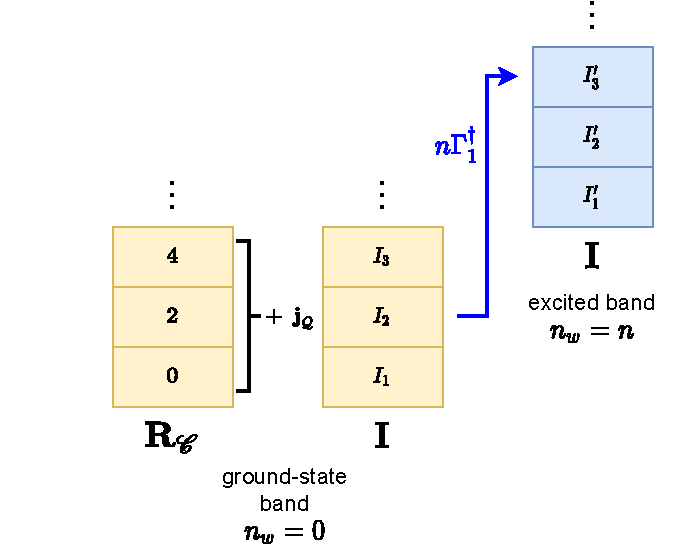
\includegraphics[width=0.75\textwidth]{Chapters/Figures/w0_phonon_operator.pdf}
    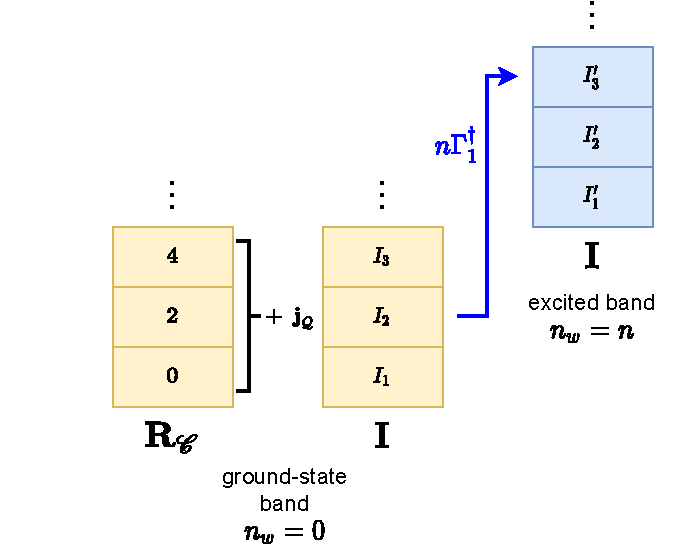
\includegraphics[width=0.9\textwidth]{Chapters/Figures/w0_phonon_operator.pdf}
    \caption{The mechanism of action for the phonon operator introduced in Ref. \cite{raduta2017semiclassical} for creating excited states of a given angular momentum, from the ground state bands. The angular momentum of the core is defined as $\mathbf{R}_\mathscr{C}$, while the quasi-particle a.m. is denoted by $\mathbf{j}_\mathcal{Q}$. The ground-state band emerges from the coupling of these two, giving rise to a series of spins $I_i=R_i+j$ (where $R=\left\{\dots,R_i-2,R_i,R_i+2\dots\right\}$). Acting with $\Gamma_1^\dagger$ $n$-times on any of these states, an excited level in the $n_w=n$ wobbling band is obtained. Keep in mind that the phonon operator increases the spin of a state by one unit. In this example a rotational core having even spin states has been chosen, however the same principle applies if the spin states are odd.}
    \label{phonon-operator-schematic}
\end{figure}

From the seminal work from 2017 of the team, several features are emphasized:
\begin{itemize}
    \item The four TSD bands are considered as zero-, one-, two-, and three-wobbling phonon bands for TSD1, TSD2, TSD3, and TSD4, respectively
    \item Each excited band is obtained by acting on the yrast (TSD1) band with one-, two-, and three-phonons, respectively (e.g., a state $I$ from TSD2 is obtained by acting with the wobbling-phonon operator on a state $I-1$ from TSD1 and so on), according to Fig. \ref{phonon-operator-schematic}
    \item Wobbling structure for the group TSD1-2-3 emerged from a proton $i_{13/2}$ ($\mathcal{Q}_p$) where all spin states have positive parity
    \item The band TSD4 has spin states with negative parity, and it is built on a proton from the $h_{9/2}$ orbital (also a $\mathcal{Q}_p$)
    \item In the expression of the rotor Hamiltonian, the rigid-like MOI were adopted (see Eq. \ref{eq-irrotational-rigid-mois}) which depend on $\gamma$ and $\mathcal{I}_0$
    \item Analytical expressions for the energies were expressed in terms of total spin and wobbling phonon numbers
    \item Experimental data was reproduced through a fitting procedure, with the free parameters $\mathcal{I}_0^{-1}$ (rotor part) and a \emph{scaling factor} $s=V\cdot \mathcal{I}_0$ (single-particle part)
    \item The model assumes similar MOI across all four bands
    \item Deformation parameters $\beta_2$ and $\gamma$ were a priori fixed (taken from literature)
\end{itemize}

A year later, the team also extended this method into analyzing the wobbling properties of two more isotopes: $^{165,167}$Lu \cite{raduta2018wobbling}, and the model showed again that it was an useful tool in providing a realistic description of the wobbling motion in odd-mass nuclei. Hereafter, when referring to the procedure realized by Raduta and Poenaru in \cite{raduta2017semiclassical} and \cite{raduta2018wobbling}, the term $\mathbf{W_0}$ will be used. Throughout the following chapters, comparisons between the newly developed theory and $\mathbf{W_0}$ will be made when necessary, in order to understand several key differences.

\section{Re-interpretation of The Wobbling Motion}

The $\mathbf{W_0}$ formalism can be regarded as a cornerstone in the description of an odd-$A$ particle-triaxial-rotor system done by the team. In a more recent follow-up work (2020) done by Raduta and Poenaru \cite{raduta2020approach,raduta2020towards}, a new interpretation of the wobbling bands was made, relative not only to $^{163}$Lu, but to an entire set of wobblers. The way of obtaining yrast and excited states within the collective spectrum turned out to be a first within literature, especially for $^{135}$Pr and $^{163}$Lu, since these nuclei have been drawing a lot of attention lately. The model starts with the typical QTR Hamiltonian:
\begin{align}
    \hat{H}=\hat{H}_\text{rot}+\hat{H}_\text{sp}\ ,
    \label{total-ham-approach-w1}
\end{align}
where $\hat{H}_\text{sp}$ represents the quasi-particle that moves inside the quadrupole mean-field as described in Eqs. \ref{eq-nilsson-ham-spherical-harmonics} and \ref{single-particle-nilsson-defored-potential} (recall discussion on the $\gamma$-deformed Nilsson potential and also Sections \ref{trm-model} - \ref{tprm-model}):
\begin{align}
    \hat{H}_\text{sp}=\epsilon_j+\frac{V}{j(j+1)}\left[\cos\gamma\left(3\hat{j}_3^3-\mathbf{j}_\mathcal{Q}^2\right)-\sqrt{3}\sin\gamma\left(\hat{j}_1^2-\hat{j}_2^2\right)\right]\ ,
    \label{single-particle-ham-approach-w1}
\end{align}
with $\epsilon_j$ as the intrinsic energy of the particle from the corresponding $j$-shell (as it was discussed in Section \ref{tprm-model}). The total angular momentum of the core + odd-particle system is $\mathbf{I}=\mathbf{R}_\mathscr{C}+\mathbf{j}_{\mathcal{Q}}$. The components of the total angular momentum are $\mathbf{I}=\{\hat{I}_1,\hat{I}_2,\hat{I}_3\}$ and the a.m. components for $\mathcal{Q}$ are $\mathbf{j}_{\mathcal{Q}}=\{\hat{j}_1,\hat{j}_2,\hat{j}_3\}$. The axes labelling for the triaxial ellipsoid is $k=(1,2,3)$. Knowing this, one can express the rotor part as \cite{raduta2020approach}:
\begin{align}
    \hat{H}_\text{rot}=\sum_{k=1}^3A_k(\hat{I}_k-\hat{j}_k)^2\ ,
    \label{rotor-ham-approach-w1}
\end{align}
where the inertial factors $A_k$ are expressed in terms of the three MOI:$$A_k=\frac{1}{2\mathcal{I}_k}\ .$$
Note that the Hamiltonian from Eq. \ref{rotor-ham-approach-w1} is just as the one expressed in Eq. \ref{general-rotor-hamiltonian}, except that here, the components of $\mathbf{R}_\mathscr{C}$ are given in terms of $\mathbf{I}$ and $\mathbf{j}_{\mathcal{Q}}$.

Obviously, the next task would be to obtain the eigenvalues of the Hamiltonian, finding thus the energies of the system. One can proceed with the diagonalization technique of $\hat{H}$ using a set of states that manifest the invariance to rotations by $\pi$ around a particular axis (the $D_2$ symmetry \cite{bohr1998nuclear}), since the Hamiltonian exhibits this property. However, it is more practical to describe the system only through a few variables that have a classical counterpart. By doing so, the system's dynamics will keep a classical analogy to that of a rotating body lacking axial symmetry. The semi-classical approach that best fits this requirement is the Variational Principle (VP), to which one associates the Time-Dependent Variational Equation (TDVE). When applying the VP on an initial problem, it is necessary to have a variational state constructed in such a way that it embeds all the relevant degrees of freedom for the underlying physics. Furthermore, the VP will induce a time dependence on the variables comprising the variational state itself \cite{budaca2018tilted}. Additionally, for each variable (usually complex) parametrizing the state, the TDVE will yield its equation of motion, thus finding the `connection' between the initial quantal variable (belonging to $S_\text{qt})$ and the classical variable (belonging to $S_\text{cls}$).

\subsection{Variational Principle}

The discussion regarding the VP and TDVE from the previous subsection can therefore be summarized in the following equation, which must be associated to the quantal Hamiltonian ($\hat{H}\subset S_\text{qt}$) defined in Eq. \ref{total-ham-approach-w1}:
\begin{align}
    \delta\int_0^t\bra{\Psi_{IM;j}}\hat{H}-i\frac{\partial}{\partial t'}\ket{\Psi_{IM;j}}dt'=0\ .
    \label{tdve-approach-w1}
\end{align}
Obviously, the variational state $\ket{\Psi_{IM;j}}$ (also known as the \emph{trial function}) must be chosen in such a way that it comprises the entire space of the original quantal Hamiltonian. This can be achieved if the function is a \emph{coherent state} \cite{glauber1963coherent}, which due to its \emph{completeness} property will span all the basis vector states from $S_\text{qt}$. Keep in mind that for $S_\text{qt}$ the states belong to the Hilbert space of $\hat{H}$. For the present case, the trial function is defined as \cite{raduta2017semiclassical}:
\begin{align}
    \Psi_\text{trial}\equiv\ket{\Psi_{IM;j}}=\mathcal{N}e^{z\hat{I}_-}e^{s\hat{j}_-}\ket{IMI}\ket{jj}\ ,
    \label{trial-function-appeoach-w1}
\end{align}
where the ladder operators for the total and single-particle a.m. are represented by $\hat{I}_-$ and $\hat{j}_-$, respectively. The subscript separated by `;' in $IM;j$ that is adopted here indicates the two different angular momenta involved in the description of the odd-mass systems (namely $\mathbf{I}$ and $\mathbf{j}_\mathcal{Q}$). The factor $\mathcal{N}$ is the normalization constant keeping the trial function normalized to unity. Its value is specified accordingly to Refs. \cite{raduta2007semiclassical,raduta2020new} as:
\begin{align}
    \mathcal{N}=\left(1+|z|^2\right)^{-I}\left(1+|s|^2\right)^{-j}\ .
\end{align}
The states $\ket{IMK}$ that are involved in $\Psi_\text{trial}$ represent the Wigner-D functions (eigenstates of $\hat{I}^2$ and $\hat{I}_3$), while $\ket{j\Omega}$ are wave-functions of the odd quasi-particle (eigenstates of $\hat{j}^2$ and $\hat{j}_3$). Notice that the trial function is explicitly given in terms of the \emph{extremal states}, i.e., the two projections are maximal $K=I$ and $\Omega=j$. The normalized states for the total angular momentum are expressed in terms of the Wigner-$\mathcal{D}$ functions \cite{ring2004nuclear}:
\begin{align}
    % \ket{IMK}=\sqrt{\frac{2I+1}{8\pi^2}}\mathcal{D}_{MK}^I\ ,\ \ket{IM-K}=\sqrt{\frac{2I+1}{8\pi^2}}\mathcal{D}_{M-K}^I\ .
    \ket{IMK}=\sqrt{\frac{2I+1}{8\pi^2}}\mathcal{D}_{MK}^I\ .
    \label{IMK-wigner-functions}
\end{align}

The vector states $\ket{j\Omega}$ describe general wave-functions for a particle $\chi$ having the structure \cite{hecht1962asymmetric}:
\begin{align}
    \ket{\chi}=\sum_{j\Omega}c_{j\Omega}\ket{j\Omega}\ ,
    % \ket{\bar{\chi}}=\sum_{j\Omega}c_{j-\Omega}\ket{\bar{\chi}_{j\Omega}}=&\sum_{j\Omega}c_{j-\Omega}\ket{j-\Omega}=\sum_{j\Omega}(-1)^{j-1/2}c_{j\Omega}\ket{j-\Omega}\ .
    \label{j-Omega-single-particle-states}
\end{align}
where the coefficients $c_{j\Omega}$ should be a priori known.
% The wave-functions are expressed in terms of the projections $\Omega=-j,\dots,j$. The states $\ket{\bar{\chi}_{j\Omega}}$ are the time-reversed ones and they are degenerate with $\ket{\chi_{j\Omega}}$. Because of the $D_2$ symmetry for $\hat{H}$, the total wave-function can be formulated as a sum over the components $K, \Omega$ and over $j$. Denoting the total wave-function of the odd-mass nucleus as $\ket{\Psi}_\text{odd}$ (not to be confused with the trial function $\Psi_\text{trial}$), it must comprise both the intrinsic ($\mathbf{I}=\mathbf{R}_\mathscr{C}+\mathbf{j}_\mathcal{Q}$) and the single-particle ($\mathbf{j}_\mathcal{Q}$) degrees of freedom, namely:
% \begin{align}
%     \ket{\Psi_\text{odd}}&=\ket{\Psi_\text{intr.}}\otimes\ket{\Psi_\mathcal{Q}}=\nonumber\\
%     &=\sqrt{\frac{2I+1}{16\pi^2}}\sum_K C_K\sum_{j\Omega}c_{j\Omega}\left[\mathcal{D}_{MK}^I\ket{\chi_{j\Omega}}+(-1)^{I-j}\mathcal{D}_{M-K}^I\ket{\bar{\chi}_{j\Omega}}\right]=\nonumber\\
%     &=\sqrt{\frac{2I+1}{16\pi^2}}\sum_K C_K \left[\mathcal{D}_{MK}^I\ket{\chi}+(-1)^{I-1/2}\mathcal{D}_{M-K}^I\ket{\bar{\chi}}\right]\ ,
%     \label{total-wavefunction-oddA-general}
% \end{align}
% where the entire summation must be evaluated under the restriction $(K-\Omega)=even$, resulting in both $K$ and $\Omega$ having the values:
% \begin{align}
%     \dots,-\frac{11}{2},-\frac{7}{2},-\frac{3}{2},\frac{1}{2},\frac{5}{2},\frac{9}{2},\frac{13}{2},\dots\ .
% \end{align}
% These states are in the quantal space $S_\text{qt}$ corresponding to the Hamiltonian from Eq. \ref{total-ham-approach-w1}. Remarking the fact that for a known quasi-particle $\mathcal{Q}$ belonging to a specific $j$-shell, one must keep $j$ constant within the summations outlined in Eq, \ref{total-wavefunction-oddA-general}.
\subsection{Classical Equations of Motion}
\label{equations-of-motion-section}

Returning to the trial function $\ket{\Psi_{IM;j}}$ from Eq. \ref{trial-function-appeoach-w1}, its expression must be further discussed in terms of the variables $z$ and $s$, which represent complex functions of time, They are associated to the motion of the core and the odd-particle, respectively, and their expressions are \cite{budaca2018tilted}:
\begin{align}
    z=\rho e^{i\varphi}\ ,\ s=\sigma e^{i\psi}\ .
    \label{z-s-variables}
\end{align}
% The next step would be to evaluate the averages of both $\hat{H}$ and the time derivative $\frac{\partial}{\partial t}$ on the variational state $\ket{\Psi_{IM;j}}$ as:
The next step would be to evaluate the averages of $\hat{H}$ on the variational state $\ket{\Psi_{IM;j}}$ as:
\begin{align}
    \left\langle \hat{H} \right\rangle&=\bra{\Psi_{IM;j}}\hat{H}\ket{\Psi_{IM;j}}\nonumber\\
    % \left\langle \frac{\partial}{\partial t} \right\rangle&=\bra{\Psi_{IM;j}}\frac{\partial}{\partial t}\ket{\Psi_{IM;j}}\ .
    \label{hamiltonian-average}
\end{align}
The analytical form of Eq. \ref{hamiltonian-average} was evaluated in Ref. \cite{raduta2017semiclassical} with respect to the variables $z$ and $s$. However, here it would be more useful to change $\rho$ and $\sigma$ in the following way:
\begin{align}
    \rho \to r&=\frac{2I}{1+\rho^2}\ ,\ 0\leq r\leq 2I\ ,\nonumber\\
    \sigma \to f&=\frac{2j}{1+\sigma^2}\ ,\ 0\leq f\leq 2j\ .
    \label{changed-rho-sigma-variables}
\end{align}
These two new variables keep the same correspondence, meaning that $r$ is related to the core and $f$ is related to the odd-particle. Moreover, by doing such a transformation, the TDVE (Eq. \ref{tdve-approach-w1}) will provide the equations of motion in a \emph{canonical form}. In fact, this is the reason behind the change of variable employed in Eq. \ref{changed-rho-sigma-variables}. The set of equations of motion is \cite{raduta2020approach}:
\begin{align}
    \frac{\partial \mathcal{H}}{\partial r}=\dot{\varphi}\ ,\ \frac{\partial \mathcal{H}}{\partial \varphi}=-\dot{r}\ ,\nonumber\\
    \frac{\partial \mathcal{H}}{\partial f}=\dot{\psi}\ ,\ \frac{\partial \mathcal{H}}{\partial \psi}=-\dot{f}\ ,
    \label{eq-of-motion-approach-w1}
\end{align}
where $\mathcal{H}$ is just the average of $\hat{H}$ on the trial function, as defined in Eq. \ref{hamiltonian-average}. It now plays the role of \emph{classical energy function} (CEF) and moreover, it is a constant of motion, implying that the energy of the system must be conserved. Remarking the fact that the \emph{classical image} of the initial problem (i.e., the Hamiltonian of an odd-$A$ triaxial nucleus) is now properly reached through the canonical equations of motion (Eq. \ref{eq-of-motion-approach-w1}). The explicit form of the equations of motion attained by the VP are \cite{raduta2020approach}:
\begin{align}
    \dot{\varphi}=&\frac{2I-1}{I}(I-r)\left(A_1\cos^2\varphi+A_2\sin^2\varphi-A_3\right)-\nonumber\\
                 &-2\sqrt{\frac{f(2j-f)}{r(2I-r)}}(I-r)\left(A_1\cos\varphi\cos\psi+A_2\sin\varphi\sin\psi\right)+2A_3(j-f)\ ,\nonumber\\
    \dot{\psi}=&\frac{2j-1}{j}(j-f)\left(A_1\cos^2\psi+A_2\sin^2\psi-A_3\right)-\nonumber\\
               &-2\sqrt{\frac{r(2I-r)}{f(2j-f)}}(j-f)\left(A_1\cos\varphi\cos\psi+A_2\sin\varphi\sin\psi\right)+2A_3(I-r)-\nonumber\\
               &-V\frac{2j-1}{j^2(j+1)}(j-f)\sqrt{3}\left(\sqrt{3}\cos\gamma+\sin\gamma\cos2\psi\right)\ , \nonumber\\
    \label{eq-of-motion-explicit-coordinates}
\end{align}
for the \emph{canonical coordinates} $(\varphi,\psi)$, and \cite{raduta2020approach}:
\begin{align}
    -\dot{r}=&\frac{2I-1}{2I}r(2I-r)(A_2-A_1)\sin2\varphi+\nonumber\\
             &+2\sqrt{rf(2I-r)(2j-f)}\left(A_1\sin\varphi\cos\psi-A_2\cos\varphi\sin\psi\right)\ ,\nonumber\\
    -\dot{f}=&\frac{2j-1}{2j}f(2j-1)(A_2-A_1)\sin2\psi+\nonumber\\
             &+2\sqrt{rf(2I-r)(2j-f)}\left(A_1\cos\varphi\sin\psi-A_2\sin\varphi\cos\psi\right)+\nonumber\\
             &+V\frac{2j-1}{j^2(j+1)}f(2j-f)\sqrt{3}\sin\gamma\sin2\psi\ ,
    \label{eq-of-motion-explicit-momenta}
\end{align}
for the \emph{canonical momenta} $(r,f)$, respectively. It results that \emph{classical coordinates} encompassed in $S_\text{cls}$ are the generalized momentum and generalized coordinates, which are represented by $(r,f)$ and $(\varphi,\psi)$, respectively. Keep in mind that the two sets of equations of motion and canonical variables correspond to the core and the single-particle. Thus, the dequantization procedure was properly described, obtaining the classical dynamics of the system.

\subsection{Classical Energy Function (CEF)}
\label{classical-energy-function-subsection}

Regarding the structure of the CEF, its expression in terms of the canonical variables is given as:
\begin{align}
    \mathcal{H}&\equiv\bra{\Psi_{IM;j}}\hat{H}\ket{\psi_{IM;j}}=\nonumber\\
    &=\frac{I}{2}(A_1+A_2)+A_3I^2+\frac{2I-1}{2I}r(2I-r)\mathcal{A}_\varphi+\frac{j}{2}(A_1+A_2)+A_3j^2+\nonumber\\
    &+\frac{2j-1}{2j}f(2j-f)\mathcal{A}_\psi-2\sqrt{rf(2I-r)(2j-f)}\mathcal{A}_{\varphi\psi}+\nonumber\\
    &+A_3\left[r(2j-f)+f(2I-r)\right]-2A_3Ij+V\frac{2j-1}{j+1}\mathcal{A}_\gamma\ .
    \label{full-classical-energy-function}
\end{align}
Since the expression is quite lengthy, some \emph{canonical factors} were introduced in Eq. \ref{full-classical-energy-function}, namely $\mathcal{A}_\varphi$, $\mathcal{A}_\psi$, $\mathcal{A}_{\varphi\psi}$, and $\mathcal{A}_\gamma$. They depend on the canonical coordinates as follows:
\begin{align}
    \mathcal{A}_\varphi&=A_1\cos^2\varphi+A_2\sin^2\varphi-A_3\ ,\nonumber\\
    \mathcal{A}_\psi&=A_1\cos^2\psi+A_2\sin^2\psi-A_3\ ,\nonumber\\
    \mathcal{A}_{\varphi\psi}&=A_1\cos\varphi\cos\psi+A_2\sin\varphi\sin\psi\ ,\nonumber\\
    \mathcal{A}_\gamma&=\cos\gamma-\frac{f(2j-f)}{2j^2}\sqrt{3}\left(\sqrt{3}\cos\gamma+\sin\gamma\cos2\psi\right)\ .
    \label{classical-energy-function-A-factors}
\end{align}

\subsubsection{Canonical Factors - Qualitative Analysis}

It is worth analyzing the behavior of the canonical factors defined in Eq. \ref{classical-energy-function-A-factors}, since their evolution with respect to the generalized coordinates and MOI ordering will provide a better understanding regarding the behavior of the CEF. Firstly, the factor $\mathcal{A}_\varphi$ is graphically represented in Fig. \ref{fig-A-varphi-canonical} for different orderings of $A_k$. Because $\mathcal{A}_\varphi$ and $\mathcal{A}_\psi$ have similar expressions (only the coordinate is changed), the plots are equivalent.
\begin{figure}
    \centering
    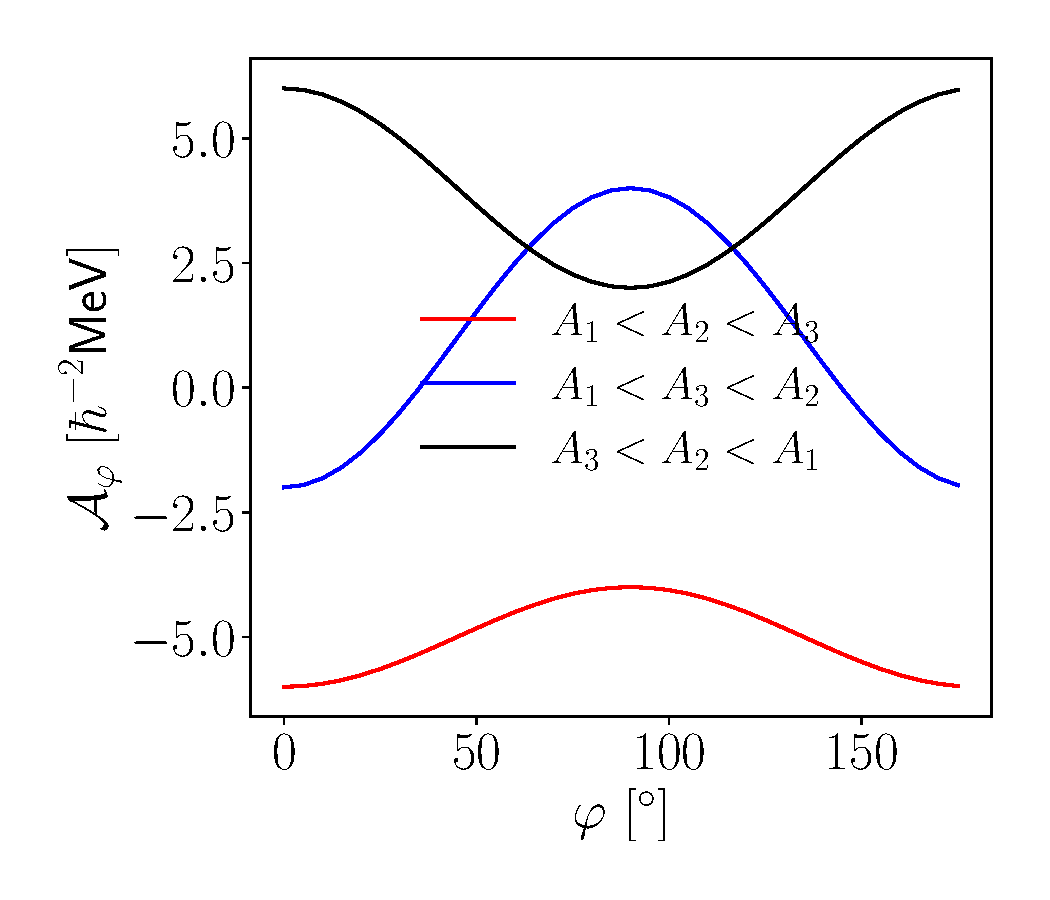
\includegraphics[width=0.49\textwidth]{Chapters/Figures/A_varphi_1.pdf}
    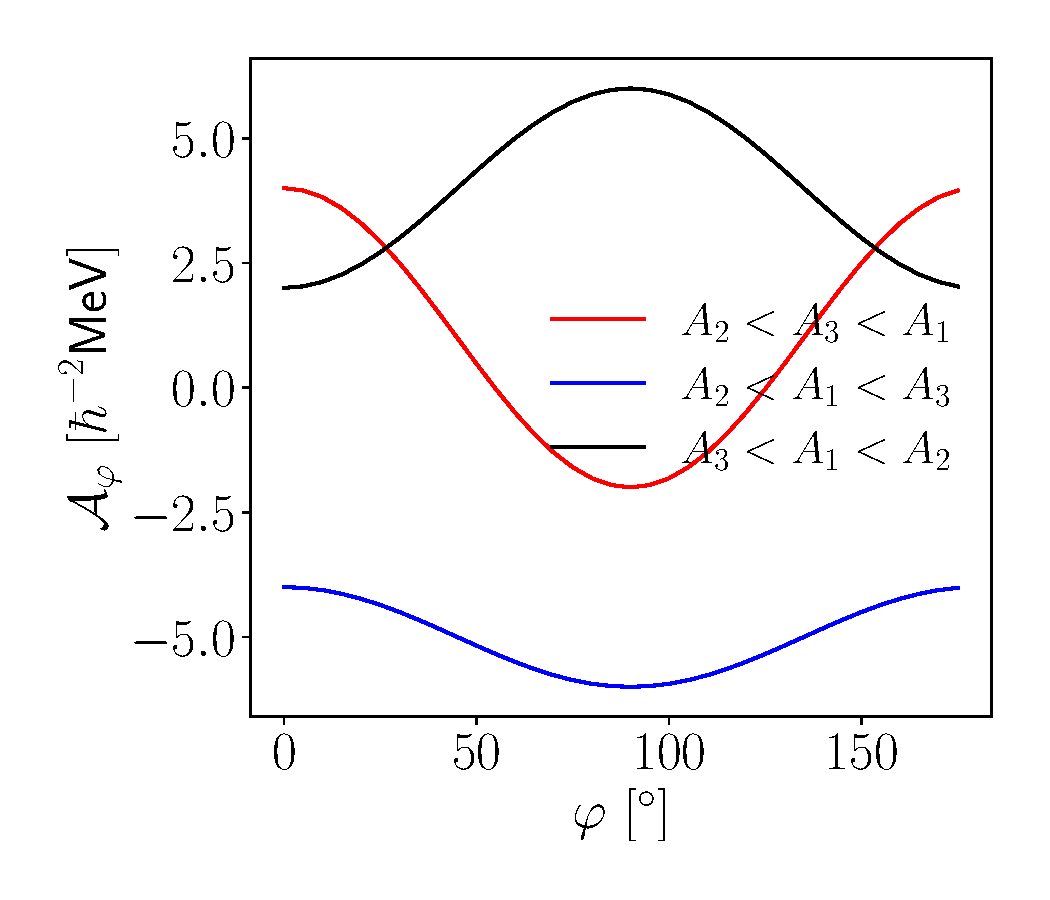
\includegraphics[width=0.49\textwidth]{Chapters/Figures/A_varphi_2.pdf}
    \caption{The evolution of $\mathcal{A}_\varphi$ with respect to the generalized coordinate $\varphi$, at different MOI orderings. The values $1,3,7$ were chosen and they are interchanged between the three inertia factors. This figure is equivalent for $\mathcal{A}_\psi$.}
    \label{fig-A-varphi-canonical}
\end{figure}

For the mixed term $\mathcal{A}_{\varphi\psi}$ from Eq. \ref{classical-energy-function-A-factors} it is more suitable to create a contour plot, as it depends on both canonical coordinates $(\varphi,\psi)$. As such, representations with different MOI orderings have been depicted in Fig. \ref{fig-A-mixed-canonical}, by lettings the coordinates vary inside the interval $[0,\pi]$.
\begin{figure}
    \centering
    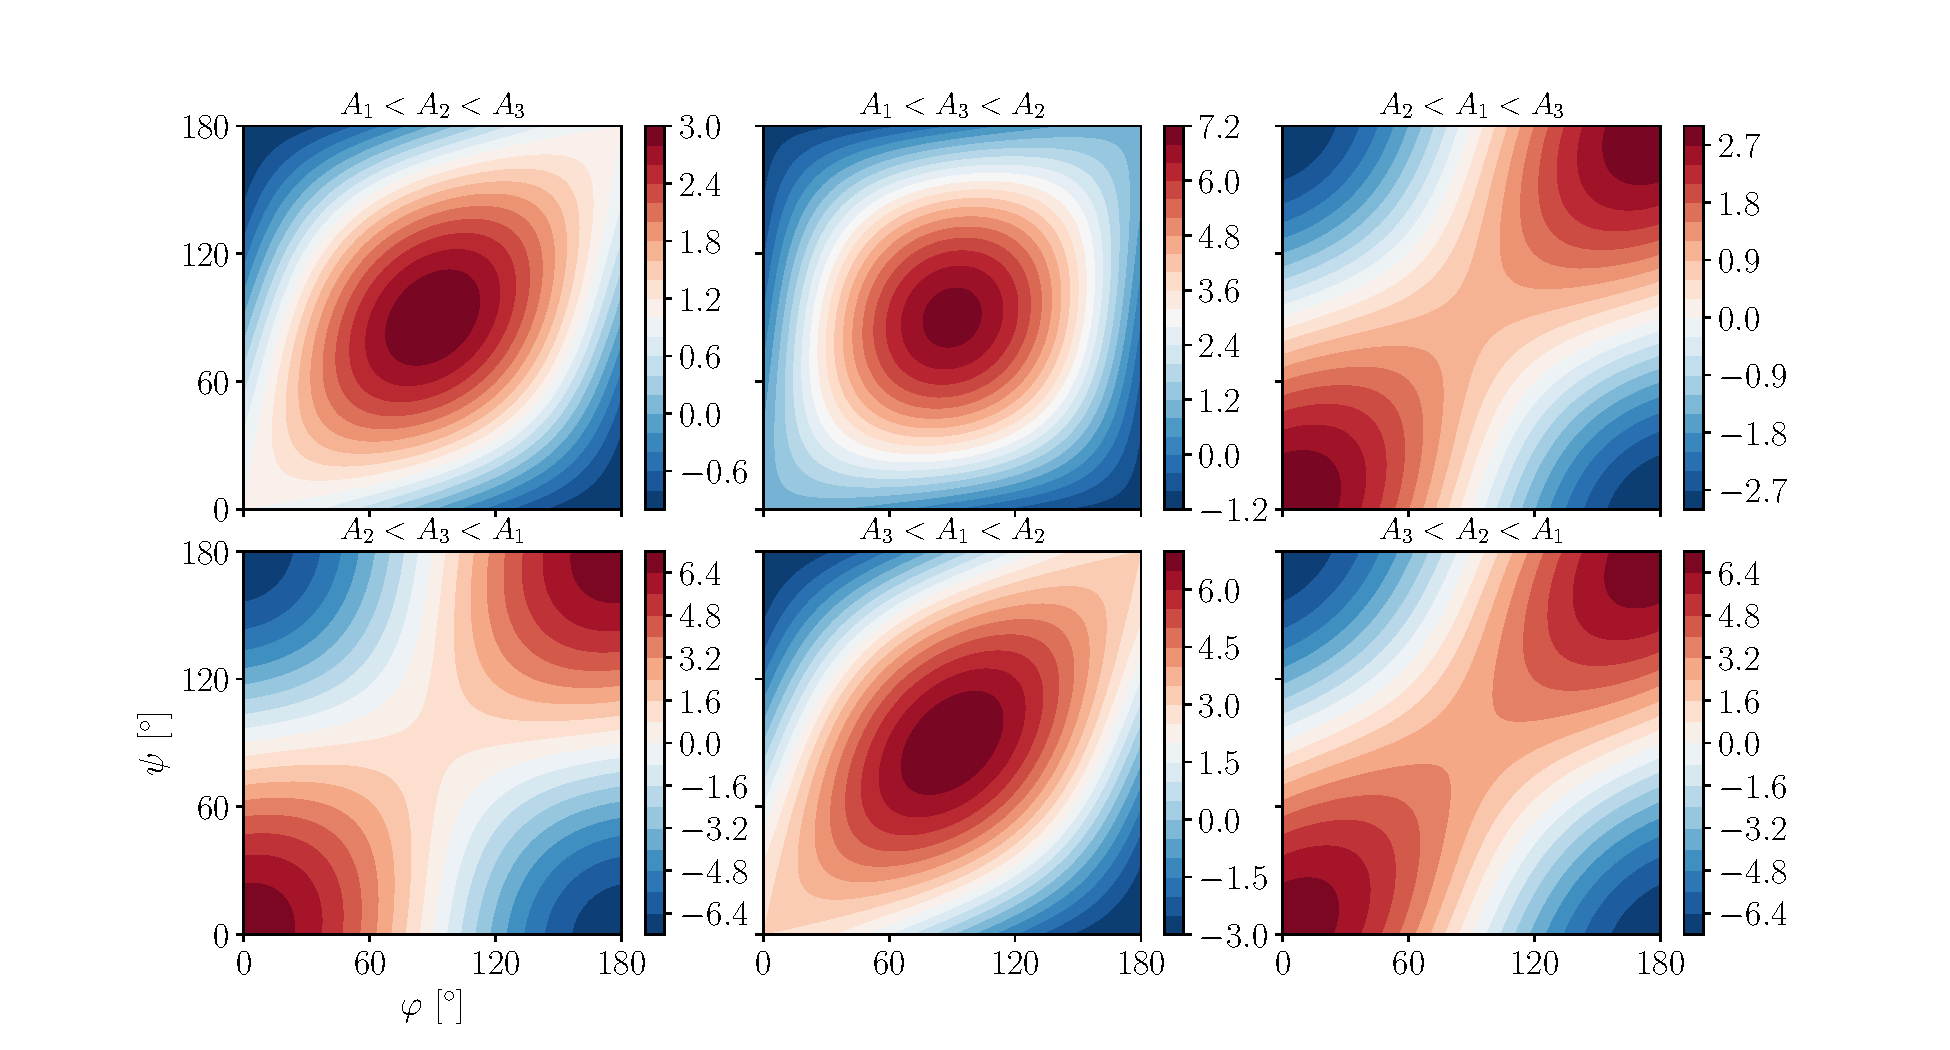
\includegraphics[width=0.99\textwidth]{Chapters/Figures/A_mixed.pdf}
    \caption{The mixed canonical factor $\mathcal{A}_{\varphi\psi}$ from Eq. \ref{classical-energy-function-A-factors}, as function of the coordinates $\varphi$ and $\psi$. Both variables vary within the interval $[0,\pi]$. All insets share a common labelling for the OX and OY axes.}
    \label{fig-A-mixed-canonical}
\end{figure}

Lastly, the factor $\mathcal{A}_{\gamma}$ must also be represented as a contour plot, because it depends on the canonical coordinates of the single-particle, namely the set $(f,\psi)$. Its graphical representation for a few values of $\gamma$ shown in Fig. \ref{fig-A-gamma-canonical}.
\begin{figure}
    \centering
    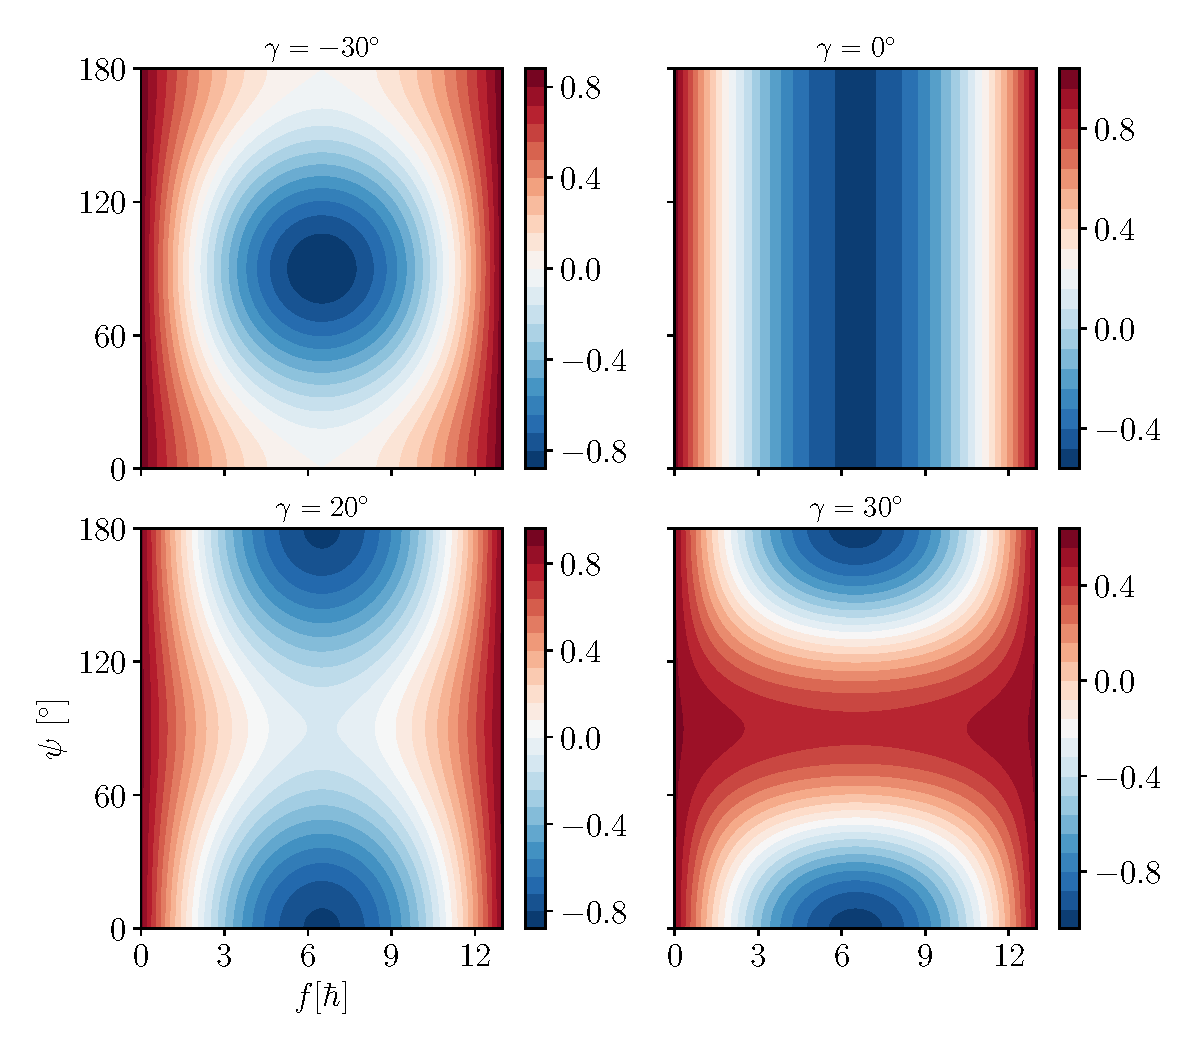
\includegraphics[width=0.99\textwidth]{Chapters/Figures/A_gamma.pdf}
    \caption{The canonical factor $\mathcal{A}_\gamma$ from Eq. \ref{classical-energy-function-A-factors}, as a function of the coordinates $(f,\psi)$ corresponding to the single-particle $\mathcal{Q}$. The $j$-shell has been fixed to $j=13/2$. In terms of the two variables, $f$ varies within $[0,2j]$ while $\psi$ is inside the interval $[0,\pi]$. All insets share a common labelling for the OX and OY axes.}
    \label{fig-A-gamma-canonical}
\end{figure}

From the representations shown in Figs. \ref{fig-A-varphi-canonical} - \ref{fig-A-gamma-canonical}, one can interpret the results as possible conditions for the stability of an odd-$A$ system in regards to the wobbling regime. More precisely, smaller values of $\mathcal{A}$ will correspond to a lower total energy. Keep in mind that all these canonical factors take part in the structure of the CEF, meaning that lower energies could imply a greater degree of stability to some extent.

\subsubsection{Critical Region}

Given the general expression of the CEF from Eqs. \ref{full-classical-energy-function} - \ref{classical-energy-function-A-factors}, one can group the terms in a part that is independent on the coordinates, a part that depends only on the core's coordinates $(r,\varphi)$, a third part that depends on the single-particle's coordinates $(f,\psi)$, and finally a \emph{mixed} term, which contains both sets of classical coordinates. As a result, $\mathcal{H}$ can be summarized (coloring is just to emphasize the grouping of the terms):
\begin{align}
    \mathcal{H}(r,\varphi;f,\psi)={\color{blue}\mathcal{H}_\text{free}}+{\color{red}\mathcal{H}_\mathscr{C}(r,\varphi)+\mathcal{H}_\mathcal{Q}(f,\psi)+\mathcal{H}_\text{mixed}(r,\varphi;f,\psi)}\ .
    \label{classical-energy-function-terms}
\end{align}
From the critical conditions associated to the classical energy function, namely:
\begin{gather*}
    \left(\frac{\partial \mathcal{H}}{\partial r}\right)=0\ ,\ \left(\frac{\partial \mathcal{H}}{\partial \varphi}\right)=0\ ,\\
    \left(\frac{\partial \mathcal{H}}{\partial f}\right)=0\ ,\ \left(\frac{\partial \mathcal{H}}{\partial \psi}\right)=0\ ,
\end{gather*}
it is possible to obtain the points at which $\mathcal{H}$ is \emph{minimal} (provided by the sign of its corresponding Hessian). In order to meet such a criteria for $\mathcal{H}$, one needs to set an ordering of the three inertia factors. Choosing the largest MOI to be around the $3$-axis and $\mathcal{I}_3>\mathcal{I}_2>\mathcal{I}_1$ (or, equivalently $A_1<A_2<A_3$), the function achieves a minimum value at:
\begin{align}
    p_0=(I,0;j,0)\ .
    \label{cef-minimum-point-p0}
\end{align}

\subsection{Wobbling Frequencies}

By performing a linearization procedure on the classical equations of motion (from Eq. \ref{eq-of-motion-approach-w1} or explicitly in Eqs. \ref{eq-of-motion-explicit-coordinates} - \ref{eq-of-motion-explicit-momenta}) around the minimum point of $\mathcal{H}$ (i.e., point $p_0$), an algebraic equation of fourth degree will show up, with a new variable which will be denoted with $\Omega$. Reasoning behind this labelling will become clear later on. For now, the equation for $\Omega$ is given generally as \cite{raduta2020towards}:
\begin{align}
    \Omega^4+B\Omega^2+C=0\ ,
    \label{omega-equation-linearized}
\end{align}
where the coefficient $B$ is \cite{raduta2020approach}:
\begin{multline}
    B=-\bigg\{\left[ (2I-1)(A_3-A_1)+2jA_1\right]\left[(2I-1)(A_2-A_1)+2jA_1\right]+8A_2A_3Ij+\\
    +\left[(2j-1)(A_3-A_1)+2IA_1+V\frac{2j-1}{j(j+1)}\sqrt{3}\left(\sqrt{3}\cos\gamma+\sin\gamma\right)\right]\times\\
    \left.\times\left[(2j-1)(A_2-A_1)+2IA_1+V\frac{2j-1}{j(j+1)}2\sqrt{3}\sin\gamma\right]\right\}\ ,
    \label{omega-B-term}
\end{multline}
and the coefficient $C$ is \cite{raduta2020approach}:
\begin{multline}
    C=\bigg\{\left[(2I-1)(A_3-A_1)+2jA_1\right]\bigg[(2j-1)(A_3-A_1)+2IA_1+\\
    +V\frac{2j-1}{j(j+1)}\sqrt{3}(\sqrt{3}\cos\gamma+\sin\gamma)\bigg]-4IjA_3^2\bigg\}\bigg\{\left[(2I-1)(A_2-A_1)+2jA_1\right]\times\\
    \times\left[(2j-1)(A_2-A_1)+2IA_1+V\frac{2j-1}{j(j+1)}2\sqrt{3}\sin\gamma\right]-4IjA_2^2\bigg\}\ .
    \label{omega-C-term}
\end{multline}
In a work done by Raduta et al \cite{raduta2017semiclassical}, a similar equation as the one from Eq. \ref{omega-equation-linearized} was obtained via a Random Phase Approximation (RPA) method applied to another (quantized) energy function. It is of crucial importance to extract from Eq. \ref{omega-equation-linearized} only those solutions that are real and positive, meaning that one has to study the stability conditions for the equation. Obviously, the general solutions are:
\begin{align}
    \Omega_1 \to \left(\frac{-B-\sqrt{B^2-4 C}}{2}\right)^{1/2}\ ,&\ \Omega_2 \to \left(\frac{-B+\sqrt{B^2-4 C}}{2}\right)^{1/2}\ ,\nonumber\\
    \Omega_3 \to -\left(\frac{-B-\sqrt{B^2-4 C}}{2}\right)^{1/2}\ ,&\ \Omega_4 \to -\left(\frac{-B+\sqrt{B^2-4 C}}{2}\right)^{1/2}\ .
    \label{omega-1-2-3-4-solutions}
\end{align}
Since the required positiveness condition, only $\Omega_1$ and $\Omega_2$ will be taken into consideration. The conditions where Eq. \ref{omega-equation-linearized} has vanishing solutions will be now analyzed in terms of $B$ and $C$.

\textit{Case i)} $B>0$ \textit{and} $C=0$

The situation $C=0$ imposes that the terms (or at least one) inside the curly brackets from Eq. \ref{omega-C-term} will equate to zero. In order to simplify the calculations, some notations should be introduced. Firstly, from the definition of $A_k=1/(2\mathcal{I}_k)$ one can exploit the fact that MOI (both in rigid representation as well as the irrotational ones) are typically expressed in terms of $\beta_2$, $\gamma$, and a common term (recall Eq. \ref{eq-irrotational-rigid-mois}):
\begin{align}
    \mathcal{I}_k=\mathcal{I}_0\cdot h(\beta_2,\gamma;k)\ ,
\end{align}
where $h$ is a trigonometric function defining moments of inertia either in the rigid picture or in the irrotational picture. Going back to the inertia factors, it results that:
\begin{align}
    A_k=\frac{1}{2\mathcal{I}_k}=\frac{1}{\mathcal{I}_0}\cdot h'(\beta_2,\gamma;k)\equiv\frac{1}{\mathcal{I}_0}\bar{A}_k\ .
    \label{A-bar-general}
\end{align}
Using Eq. \ref{A-bar-general} it is possible to rewrite each sub-term from $B$ and $C$ with the following notations:
\begin{align}
    P_{31}&=(2I-1)(\bar{A}_3-\bar{A}_1)+2j\bar{A}_1\ ,\ P_{21}=(2I-1)(\bar{A}_2-\bar{A}_1)+2j\bar{A}_1\ , \nonumber\\
    Q_{31}&=(2j-1)(\bar{A}_3-\bar{A}_1)+2I\bar{A}_1\ ,\ Q_{21}=(2j-1)(\bar{A}_2-\bar{A}_1)+2I\bar{A}_1\ ,\nonumber\\
    G_1&=\frac{2j-1}{j(j+1)}\sqrt{3}\left(\sqrt{3}\cos\gamma+\sin\gamma\right)\ ,\ G_2=\frac{2j-1}{j(j+1)}2\sqrt{3}\sin\gamma\ .
    \label{P-Q-G1-G2-factors}
\end{align}
This transformation is very useful because the constant $1/\mathcal{I}_0$ can be factored out from both $B$ and $C$, leaving only one `independent variable' within equations, i.e., $S=\mathcal{I}_0V$, which will be considered a \emph{scaling factor}. Getting back to $C=0$, after some rearrangement one gets:
\begin{align}
    P_{31}G_1S+P_{31}Q_{31}-4Ij\bar{A}_3^2=&0\ ,\nonumber\\
    P_{21}G_2S+P_{21}Q_{21}-4Ij\bar{A}_2^2=&0\ .
    \label{S-parameter-equations-set1}
\end{align}
Indeed, the above formulas represent a set of linear equations in the newly introduced variable $S$, which are of the form $aS+b=0$. As a physical interpretation for $S$, it is remarkable the fact that it comprises a rotational part of the odd-mass system (through $\mathcal{I}_0$) and also single-particle contribution (through the potential strength $V$) such that it \emph{embeds} both the effect of collective rotation and deformation. By a straightforward manipulation of Eq. \ref{S-parameter-equations-set1}, the two solutions which provide vanishing a $C$ term are:
\begin{align}
    S_{01}=\frac{4Ij\bar{A}_3^2-P_{31}Q_{31}}{P_{31}G_1}\ \text{and}\ S_{02}=\frac{4Ij\bar{A}_2^2-P_{21}Q_{21}}{P_{21}G_2}\ .
    \label{C-Term-zero-solutions}
\end{align}

\textit{Case ii)} $B=0$ \textit{and} $C=\text{arbitrary}$

When $B$ must vanish, a second-degree algebraic equation for the variable $S$ will emerge. Using the same notations that where introduced in the case $i)$ for the sub-terms involved in $C$, it results the following:
\begin{align}
    P_{31}P_{21}+8Ij\bar{A}_2\bar{A}_3+\left(Q_{31}+SG_1\right)\left(Q_{21}+SG_2\right)=0\ , \nonumber
\end{align}
or, after some manipulation:
\begin{align}
    G_1G_2S^2+\left(Q_{21}G_1+Q_{31}G_2\right)S+P_{31}P_{21}+8Ij\bar{A}_2\bar{A}_3=0\ .
    \label{S-parameter-equations-set2}
\end{align}
The solutions of this second-degree equation are:
\begin{align}
    S_{11}&=-\frac{\sqrt{\left(G_1 Q_{21}+G_2 Q_{31}\right){}^2-4 G_1 G_2 \left(8 I j \bar{A}_2 \bar{A}_3+P_{21} P_{31}\right)}+G_1 Q_{21}+G_2 Q_{31}}{2 G_1 G_2}\ ,\nonumber\\
    S_{12}&=\frac{\sqrt{\left(G_1 Q_{21}+G_2 Q_{31}\right){}^2-4 G_1 G_2 \left(8 I j \bar{A}_2 \bar{A}_3+P_{21} P_{31}\right)}-G_1 Q_{21}-G_2 Q_{31}}{2 G_1 G_2}\ .
    \label{B-Term-zero-solutions}
\end{align}

Gathering the outcomes of Eqs. \ref{C-Term-zero-solutions} and \ref{B-Term-zero-solutions}, four solutions for the variable $S$ are obtained, i.e., $S=\{S_{01},S_{02},S_{11},S_{12}\}$. Returning to the case $i)$ that provides a vanishing $C$ term, it would be instructive to see for what values of $\mathcal{I}_0$ and $V$ the left-hand sides from Eq. \ref{S-parameter-equations-set1} equate to zero. Denoting the first left-hand side with $f_1=f_1(\mathcal{I}_0,V)$ and the second one with $f_2=f_2(\mathcal{I}_0,V)$, a contour plot in the $(\mathcal{I}_0,V)$ space can be developed, where any contour line would depict the regions at which $f_1$ and $f_2$ are null. This is graphically represented in the left inset of Fig. \ref{fig-vanishing-f1-f2-F}, revealing that for $\mathcal{I}_0\in[0,60]$, the value of $V$ does not change and the contours consist of straight lines, which is indeed noteworthy. In order to distinguish the positive/negative regions of $f_1$ and $f_2$, a 50-50 ratio of red-blue colors has been chosen relative to the width of the plot. Nevertheless, both terms cover the entire range of values provided for $V$ and $\mathcal{I}_0$.

Furthermore, the left-hand side of Eq. \ref{S-parameter-equations-set2} from case $ii)$ can also be zero for certain intervals of $\mathcal{I}_0$ and $V$. A restriction on $V$ to only have positive values is adopted throughout the formalism (to be consistent with the literature \cite{shou2009coupling,tanabe2017stability,poenaru2021parity}). This forces only a single contour (denoted with $F=0$) to appear above the OX axis. A representation showing this line is done in the right inset of Fig. \ref{fig-vanishing-f1-f2-F}. Keep in mind that the $V$ parameter is restricted to the interval $[0,5]$.
\begin{figure}
    \centering
    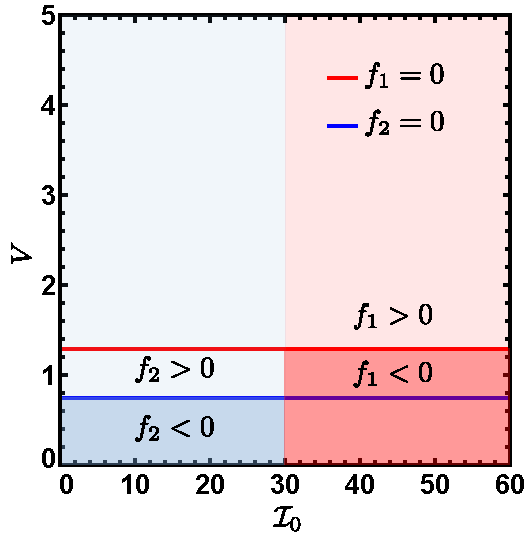
\includegraphics[width=0.49\textwidth]{Chapters/Figures/f1f2_solutions-edited.pdf}
    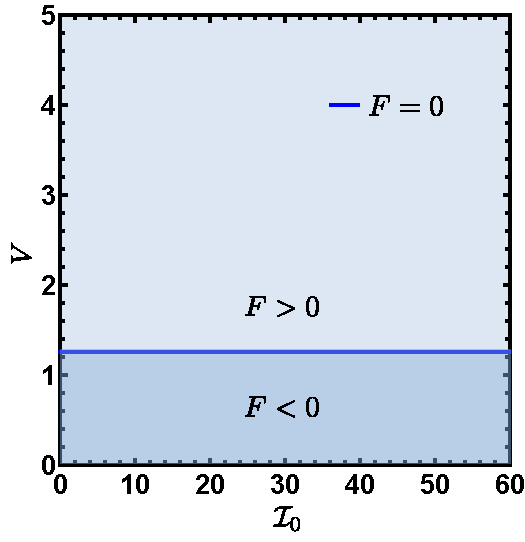
\includegraphics[width=0.49\textwidth]{Chapters/Figures/F_solutions_B-term.pdf}
    \caption{\textbf{Left:} The contour lines that show for what values of $\mathcal{I}_0$ and $V$ the left-hand sides from Eq. \ref{S-parameter-equations-set1} are zero. The two sides are denoted here by $f_1$ and $f_2$, respectively. \textbf{Right:} Graphical representation with the contour $F=0$ as function of the parameters $\mathcal{I}_0$ and $V$, where $F$ represents the left-hand side of Eq. \ref{S-parameter-equations-set2}. \textbf{Both:} Darker (lighter) color corresponds to negative (positive) values. The calculations were done for fixed values of $I, j, \gamma, A_1, A_2, A_3$. Units are $\hbar^2\text{MeV}^{-1}$ for $\mathcal{I}_0$ and $\text{MeV}$ for $V$.}
    \label{fig-vanishing-f1-f2-F}
\end{figure}

Taking a look at the regions portrayed in Fig. \ref{fig-vanishing-f1-f2-F}, one can assume that they represent a clear indicator concerning the stability of Eq. \ref{omega-equation-linearized}. Obviously, when the values of $(\mathcal{I}_0,V)$ lie near the contours lines, then the equation reaches instability and no real solutions emerge.

Regarding the solutions given in Eq. \ref{omega-1-2-3-4-solutions}, the selected ones are $\Omega_1$ and $\Omega_2$. Considering their structure, it is important to retrieve all the conditions that grant positive square roots. These conditions are sketched in Table \ref{omega-positive-conditions}.
\begin{table}
    \centering
    \resizebox{0.69\textwidth}{!}{%
    \begin{tabular}{|c|c|}
    \hline
    Solution   & Positive square root \\ \hline
    $\Omega_1$ & $B<0\ \text{and}\ 0\leq C\leq \frac{B^2}{4}$                      \\ \hline
    $\Omega_2$ & $\left(B\leq 0\ \text{and}\ C\leq \frac{B^2}{4}\right)$ or $\left(B<0\ \text{and}\ C\leq 0\right)\ $                     \\ \hline
    \end{tabular}%
    }
    \caption{The conditions for which the square roots that appear in the two solutions $\Omega_{1,2}$ given in Eq. \ref{omega-1-2-3-4-solutions} are positive, such that real quantities can be obtained. The trivial solution $B=C=0$ has been dismissed.}
    \label{omega-positive-conditions}
\end{table}

Going back to the CEF in the form shown in Eq. \ref{classical-energy-function-terms}, the free term $\mathcal{H}_\text{free}$ is the one that does not depend on any canonical variable. The other three terms (depicted by red color) have a dependence on either the core's coordinates $(r,\varphi)$ or the particle's coordinates $(f,\psi)$. However, the remarking feature is that all these terms are comprised in the two solutions $\Omega_1$ and $\Omega_2$. In fact, one expects such a thing because $\Omega_1$ and $\Omega_2$ emerge from the linearization of the equations of motion around the minimum point $p_0=(r_0=I,\varphi_0=0\ ;\ f_0=j,\psi_0=0)$. As it was shown in $\mathbf{W_0}$ and also Refs. \cite{raduta2020approach,raduta2020new}, the solutions $\Omega_{1,2}$ give the `final' terms in the total energy spectrum for an odd-mass system. More precisely, the CEF from \ref{classical-energy-function-terms} combined with the two real and positive solutions of Eq. \ref{omega-equation-linearized} will result in the spectrum \cite{poenaru2021extensive1}:
\begin{align}
    E_{I,n_1,n_2}=\epsilon_j+{\color{blue}\mathcal{H}_\text{min}^I}+{\color{red}\mathcal{F}^I_{n_{w_1}n_{w_2}}}\ ,
    \label{tsd-bands-compressed-spectrum}
\end{align}
where the free term given in Eq. \ref{classical-energy-function-terms} becomes the \emph{minimal energy} $\mathcal{H}_\text{min}^I$ and the \emph{phonon} term $\mathcal{F}_{n_{w_1}n_{w_2}}^I$ is the sum of the two solutions $\Omega_{1,2}$ \cite{poenaru2021extensive1}:
\begin{align}
    \mathcal{F}_{n_{w_1}n_{w_2}}^I=\hbar\Omega_1^I\left(n_{w_1}+\frac{1}{2}\right)+\hbar\Omega_2^I\left(n_{w_2}+\frac{1}{2}\right)\ .
    \label{phononic-term-tsd-energies}
\end{align}

The term from Eq. \ref{phononic-term-tsd-energies} can be regarded as originating from $\mathcal{H}_\mathscr{C}+\mathcal{H}_\mathcal{Q}+\mathcal{H}_\text{mixed}$. This was obtained from the linearization procedure mentioned at the start of the section. The energy of the odd-particle belonging to a particular $j$-shell (as per $\hat{H}_\text{sp}$ from Eq. \ref{single-particle-ham-approach-w1}) is represented by $\epsilon_j$, which should be adopted as a constant. The coloring from Eq. \ref{tsd-bands-compressed-spectrum} is consistent with the one from Eq. \ref{classical-energy-function-terms} such that the analogy between each component can be clearly viewed. Putting together Eq. \ref{tsd-bands-compressed-spectrum} and Eq. \ref{phononic-term-tsd-energies}, the general spectrum of an odd-mass triaxial nucleus will be:
\begin{align}
    E_{I,n_1,n_2}=\epsilon_j+\mathcal{H}_\text{min}^I+\hbar\Omega_1^I\left(n_{w_1}+\frac{1}{2}\right)+\hbar\Omega_2^I\left(n_{w_2}+\frac{1}{2}\right)\ .
    \label{tsd-bands-general-spectrum}
\end{align}
The conditions for which $\Omega_{1,2}$ exist and meet the criteria of positiveness were summarized in Table \ref{omega-positive-conditions}. The physical interpretation of $\Omega_1$ and $\Omega_2$ from Eq. \ref{tsd-bands-general-spectrum} is a remarking feature of this formalism. Indeed, here $\Omega$ represents a wobbling frequency, in the same manner as for the simple wobbler (recall Eq. \ref{eq-wobbling-energy-evenA}) or the odd-$A$ case discussed in Chapter \ref{chapter-5} (see Section \ref{chapter-5-odd-wobbling-theory}). The advantage of using the TDVE approach is that the Hamiltonian is properly `split' and two wobbling frequencies emerge: one for the core and one for the odd particle. This semi-classical approach is very useful for visualizing the two interacting systems directly from the analytical expression (i.e., Eq. \ref{tsd-bands-general-spectrum}) of the spectrum. In contrast, the odd-$A$ theory depicted in Chapter \ref{chapter-5} resulted in a singular wobbling frequency for the QTR Hamiltonian (see Eq. \ref{wobbling-freq-oddA}), and the interplay between the core and the particle was not clearly separated.

Concerning the two numbers from Eq. \ref{tsd-bands-general-spectrum}, i.e., $n_{w_1}=0,1,\dots$ and $n_{w_2}=0,1,\dots$, they are the wobbling phonon numbers, which are also separated in terms of the core and the single-particle. These integers represent the number of excited quanta, and the triaxial bands will be built with such quanta. 
% The entire discussion for obtaining the energy spectrum for a triaxial system, starting from the dequantization of $\hat{H}$ and ending with the two harmonic frequencies for the core and the particle, can be summarized in a diagram where the steps are schematically shown together with a final physical interpretation of $\Omega_{1,2}$ and $n_{w_{1,2}}$. The resulting drawing is shown in Fig. \ref{TDVE-wobbling-complete-sketch}.
% \begin{figure}
%     \centering
%     % \includegraphics[]{}
%     \caption{\textbf{TO FINISH: }An illustration depicting the dequantization of the initial Hamiltonian for an odd-mass triaxial nucleus. From the classical canonical variables given by TDVE, a set of two wobbling frequencies are obtained, which are ascribed to the even-even core and the single-particle. Each frequency can be regarded as a precessional motion of either $\mathbf{R}_\mathscr{C}$ or $\mathbf{j}_\mathcal{Q}$.}
%     \label{TDVE-wobbling-complete-sketch}
% \end{figure}

\subsection{Alternative Approach}
\label{Omega-1-2-alternative-method}

In the following, a different description for the phonon term $\mathcal{F}_{n_{w_1}n_{w_2}}^I$ from Eq. \ref{phononic-term-tsd-energies} will be made and, nevertheless, the method will provide similar results regarding $\Omega_1$ and $\Omega_2$. This approach will help to understand the definition of the wave-functions of the triaxial bands that will be described later on. Starting again with the CEF from Eq. \ref{classical-energy-function-terms} and expanding it around $p_0$ up to second order, the obtained equation will be \cite{raduta2020approach}:
\begin{align}
    \mathcal{H}=&{\color{blue}\mathcal{H}_\text{min}^I}+\nonumber\\
                &+{\color{red}\bigg\{}\frac{1}{2I}\left[(2I-1)(A_3-A_1)+2jA_1\right]r'^{2}+\frac{I}{2}\left[(2I-1)(A_2-A_1)+2jA_1\right]\varphi'^2+\nonumber\\
                &+\frac{1}{2j}\left[(2j-1)(A_3-A_1)+2IA_1+V\frac{2j-1}{j(j+1)}\sqrt{3}\left(\sqrt{3}\cos\gamma+\sin\gamma\right)\right]f'^2+\nonumber\\
                &+\frac{j}{2}\left[(2j-1)(A_2-A_1)+2IA_1+V\frac{2j-1}{j(j+1)}2\sqrt{3}\sin\gamma\right]\psi'^2-\nonumber\\
                &-2A_3r'f'-2IjA_2\varphi'\psi'{\color{red}\bigg\}}\ .
    \label{classical-energy-function-deviations}
\end{align}
where the primed coordinates $r',\varphi',f',\psi'$ are the deviations from the minimum point $p_0=(r_0,\varphi_0;f_0,\psi_0)$, which are expressed as:
\begin{align}
    r'=(r-r_0)\ ,\ \varphi'=(\varphi-\varphi_0)\ ,\nonumber\\
    f'=(f-f_0)\ ,\ \psi'=(\psi-\psi_0)\ .
\end{align}
Note that the curly brackets from Eq. \ref{classical-energy-function-deviations} are used to emphasize the three terms $\mathcal{H}_\mathscr{C}(r,\varphi)+\mathcal{H}_\mathcal{Q}(f,\psi)+\mathcal{H}_\text{mixed}(r,\varphi;f,\psi)$, so that one can clearly see the which are the terms with separated canonical variables and which are the mixed ones. Again one illustrates the grouped factors as per Eq. \ref{classical-energy-function-terms} through a similar coloring. It is clear from this expression that $\mathcal{H}_\text{min}^I$ is the free term $\mathcal{H}_\text{free}$.

\paragraph*{\textit{i) Non-coupling terms}}
Ignoring the coupling terms from Eq. \ref{classical-energy-function-deviations}, the CEF will consist in the sum of two independent harmonic oscillators with the frequencies:
\begin{align}
    \omega_1=&\left\{\left[(2I-1)(A_3-A_1)+2jA_1\right]\left[(2I-1)(A_2-A_1)+2jA_1\right]\right\}^{1/2}\ ,\nonumber\\
    \omega_2=&\left[(2j-1)(A_3-A_1)+2IA_1+V\frac{2j-1}{j(j+1)}\sqrt{3}\left(\sqrt{3}\cos\gamma+\sin\gamma\right)\right]^{1/2}\cdot\nonumber\\
    &\cdot\left[(2j-1)(A_2-A_1)+2IA_1+V\frac{2j-1}{j(j+1)}2\sqrt{3}\sin\gamma\right]^{1/2}\ .
    \label{small-omega-1-2}
\end{align}

In order to obtain real solutions for $\omega_1$, the following conditions for the three inertia factors must hold:
\begin{align}
    A_3>SA_1\ \text{and}\ \ A_2>SA_1\ ,\nonumber\\
    \text{while:}\ A_3>A_2\ \text{or}\ A_3<A_2\ ,
\end{align}
while for the second frequency, the following restrictions must hold:
\begin{align}
    A_3>&S'A_1-VT\ \text{and}\ A_2>S'A_1-VT'\ ,\nonumber
    % &\text{while:}\ A_3>A_2\ \text{or}\ A_3<A_2\ ,
\end{align}
with the terms $S$, $S'$, $T$, and $T'$ defined as:
\begin{align}
    S=\frac{2I-1-2j}{2I-1}\ &,\  S'=\frac{2j-2I-1}{2j-1}\ ,\nonumber\\
    T=\frac{1}{j(j+1)}\sqrt{3}\left(\sqrt{3}\cos\gamma+\sin\gamma\right)\ &,\ T'=\frac{1}{j(j+1)}2\sqrt{3}\sin\gamma\ .
\end{align}
The positiveness for $V$ will make sure that the conditions given for $\omega_2$ are always satisfied.

\paragraph*{\textit{ii) Coupling terms}}
For treating the terms from the expansion given in Eq. \ref{classical-energy-function-deviations} that contain products of the type $r'\cdot f'$ and $\varphi'\cdot \psi'$, a \emph{quantization} should be employed on the canonical variables. Indeed, from the classical coordinates (obtained via the TDVE) of the phase space $S_\text{cls}$, one can also go back to a quantum $S_\text{qt}$ space, where each coordinate will have a corresponding (quantal) operator defined in that space. Such a change was properly implemented in \cite{raduta2020approach}, resulting in the following transformations:
\begin{align}
    \varphi\to\hat{q}_1\ ,\ r\to\hat{p}_1\ ,\ \left[\hat{q}_1,\hat{p}_1\right]&=\iu\ ,\nonumber\\
    \psi\to\hat{q}_2\ ,\ f\to\hat{p}_2\ ,\ \left[\hat{q}_2,\hat{p}_2\right]&=\iu\ .
    \label{canonical-coordinates-quantized}
\end{align}
The notation of the operators is consistent with the fact that $(\varphi,\psi)$ represent the canonical coordinates and $(r,f)$ depict the canonical momenta. Furthermore, each set has a corresponding creation and annihilation operator defined as:
\begin{align}
    a^\dagger=\frac{1}{\sqrt{2}k_1}\left(k_1^2\hat{q}_1+ \iu \hat{p}_1\right)\ ,\ a=\frac{1}{\sqrt{2}k_1}\left(k_1^2\hat{q}_1+ \iu \hat{p}_1\right)\ ,
    \label{creation-operators-a}
\end{align}
for the variables $(r,\varphi)$ of the core and:
\begin{align}
    b^\dagger=\frac{1}{\sqrt{2}k_2}\left(k_2^2\hat{q}_2+ \iu \hat{p}_2\right)\ ,\ b=\frac{1}{\sqrt{2}k_2}\left(k_2^2\hat{q}_2+ \iu \hat{p}_2\right)\ ,
    \label{creation-operators-b}
\end{align}
for the single-particle variables $(f,\psi)$. Using the terms defined in Eqs. \ref{creation-operators-a} - \ref{creation-operators-b}, the operators $(\hat{q}_1,\hat{p}_1)$ and $(\hat{q}_2,\hat{p}_2)$ will acquire the following form:
\begin{align}
    \hat{q}_1=&\frac{1}{\sqrt{2}k_1}\left(a^\dagger+a\right)\ ,\ \hat{p}_1=\frac{\iu k_1}{\sqrt{2}}\left(a^\dagger-a\right)\ ,\nonumber\\
    \hat{q}_2=&\frac{1}{\sqrt{2}k_2}\left(b^\dagger+b\right)\ ,\ \hat{p}_2=\frac{\iu k_2}{\sqrt{2}}\left(b^\dagger-b\right)\ .
    \label{canonical-transformations-ab-qp}
\end{align}

The transformations that go from $(\hat{q}_1,\hat{p}_1)$ and $(\hat{q}_2,\hat{p}_2)$ to $(a^\dagger, a)$ and $(b^\dagger, b)$ are \emph{canonical}. The two constant factors $k_1$ and $k_2$ that appear in Eqs. \ref{creation-operators-a} - \ref{canonical-transformations-ab-qp} are called \emph{canonicity factors} \cite{raduta2017semiclassical}, and they are fixed such that `dangerous' terms like $(a^\dagger)^2+a^2$ and $(b^\dagger)^2+b^2$ do not appear in the two frequencies. One should not confuse them with the canonical factors $\mathcal{A}$, which were defined in Eq. \ref{classical-energy-function-A-factors} as a way of expressing the CEF. The expressions for $k_1$ and $k_2$ are \cite{raduta2020approach}:
\begin{align}
    k_1=&\left[\frac{(2I-1)(A_2-A_1)+2jA_1}{(2I-1)(A_3-A_1)+2jA_1}\cdot I^2\right]^{1/4}\, \nonumber\\
    k_2=&\left[\frac{(2j-1)(A_2-A_1)+2IA_1+V\frac{2j-1}{j(j+1)}2\sqrt{3}\sin\gamma}{(2j-1)(A_3-A_1)+2IA_1+V\frac{2j-1}{j(j+1)}\sqrt{3}\left(\sqrt{3}\cos\gamma+\sin\gamma\right)}\cdot j^2\right]^{1/4}\ .
    \label{canonicity-factors}
\end{align}
It can be seen that the canonicity factors from Eq. \ref{canonicity-factors} exhibit a behavior $f(x)\propto x^{1/2}$ with respect to the total and single-particle angular momentum, respectively. Moreover, the triaxiality parameter and the single-particle potential strength only affect $k_2$.
% which is consistent with the particle + core system, i.e., the single-particle will drive the entire system to a large degree of deformation and it will stabilize the structure. 
In a similar fashion as for the calculations done in Eqs. \ref{S-parameter-equations-set1} and \ref{S-parameter-equations-set2}, one can introduce a set of additional notations:
\begin{align}
    \Delta_{31}=&(2I-1)(A_3-A_1)+2jA_1\ ,\ \Delta_{21}=(2I-1)(A_2-A_1)+2jA_1\ ,\nonumber\\
    \Sigma_{31}=&(2j-1)(A_3-A_1)+2IA_1\ ,\ \Sigma_{21}=(2j-1)(A_2-A_1)+2IA_1\ ,
    \label{Sigma-Delta-factors}
\end{align}
where the factors $G_1$ and $G_2$ from Eq. \ref{P-Q-G1-G2-factors} will be kept the same. Compared to the calculations from Eqs. \ref{S-parameter-equations-set1} - \ref{S-parameter-equations-set2}, no prior factorization for the inertia factors is made here. With the notations given in Eq. \ref{Sigma-Delta-factors}, the two oscillator frequencies and the canonicity factors achieve a more practical shape, namely:
\begin{align}
    \omega_1=&\left(\Delta_{31}\cdot\Delta_{21}\right)^{1/2}\ ,\nonumber\\
    \omega_2=&\left(\Sigma_{31}+VG_1\right)^{1/2}\cdot\left(\Sigma_{21}+VG_2\right)^{1/2}\ ,
\end{align}
for the wobbling frequencies, and:
\begin{align}
    k_1=&\left(\frac{\Delta_{21}}{\Delta_{31}}\cdot I^2\right)^{1/4}\, \nonumber\\
    k_2=&\left[\frac{\Sigma_{21}+VG_2}{\Sigma_{31}+VG_1}\cdot j^2\right]^{1/4}\ ,
\end{align}
for the two canonicity factors. Notice the single-particle strength appearing explicitly for $\omega_2$ and also $k_2$.

From the quantization made in Eq. \ref{canonical-coordinates-quantized}, the operators $(a^\dagger,a;b^\dagger,b)$ defined in Eqs. \ref{creation-operators-a} - \ref{creation-operators-b}, and the factors defined in Eq. \ref{canonicity-factors}, this \emph{new quantal representation} of the classical energy $\left\{S_\text{cls}\supset\mathcal{H}\right\}\to\left\{\hat{H}\subset S_\text{qt}\right\}$ will achieve the following form:
\begin{align}
    \hat{H}={\color{blue}\mathcal{H}_\text{min}^I}+{\color{red}\bigg\{}\omega_1\left(a^\dagger a+\frac{1}{2}\right)+&\omega_2\left(b^\dagger b+\frac{1}{2}\right)+A_3k_1k_2\left(a^\dagger b^\dagger+ba-a^\dagger b-b^\dagger a\right)-\nonumber\\
                                                                                &-IjA_2\frac{1}{k_1k_2}\left(a^\dagger b^\dagger + ba + a^\dagger b + b^\dagger a \right){\color{red}\bigg\}}\ .
    \label{quantized-Hamiltonian-CEF}
\end{align}
Since $\mathcal{H}_\text{min}^I$ does not depend on the canonical variables, its structure will stay unchanged. The next two terms are the harmonic oscillators with the two frequencies of oscillation $\omega_1$ and $\omega_2$, while the last two contain mixed products of creation/annihilation operators from both the core and single-particle degrees of freedom. Indeed, this structure can be regarded in a similar way as the grouped terms from Eq. \ref{classical-energy-function-terms} or Eq. \ref{classical-energy-function-deviations}, depicted here by the blue and red colors. The Hamiltonian defined in Eq. \ref{quantized-Hamiltonian-CEF} will have the following commutation rules with the creation and annihilation operators:
\begin{align}
    \left[\hat{H},a^\dagger\right]=&\omega_1a^\dagger+A_3k_1k_2(b-b^\dagger)-IjA_2\frac{1}{k_1k_2}(b+b^\dagger)\ ,\nonumber\\
    \left[\hat{H},a\right]=&-\omega_1a-A_3k_1k_2(b^\dagger-b)+IjA_2\frac{1}{k_1k_2}(b^\dagger+b)\ ,\nonumber\\
    \left[\hat{H},b^\dagger\right]=&\omega_2b^\dagger+A_3k_1k_2\left(a-a^\dagger\right)-IjA_2\frac{1}{k_1k_2}\left(a+a^\dagger\right)\ ,\nonumber\\
    \left[\hat{H},b\right]=&-\omega_2b-A_3k_1k_2\left(a^\dagger-a\right)+IjA_2\frac{1}{k_1k_2}\left(a^\dagger+a\right)\ .
    \label{H-quantal-linear-system-a-b-operators}
\end{align}

One can see that Eq. \ref{H-quantal-linear-system-a-b-operators} forms a linear system, which can be solved with the introduction of a special \emph{phonon operator} \cite{raduta2017semiclassical,raduta2018wobbling}:
\begin{align}
    \Gamma^\dagger=X_1a^\dagger-Y_1a+X_2b^\dagger-Y_2b\ .
\end{align}
The four \emph{phonon amplitudes} $(X_1,Y_1)$ and $(X_2,Y_2)$ are complex numbers defined in such a way that the following restrictions (commutation rules) hold true:
\begin{align}
    \left[\hat{H},\Gamma^\dagger\right]=\Omega\Gamma^\dagger\ ,\ \left[\Gamma,\Gamma^\dagger\right]=1\ ,
    \label{H-Gamma-phonon-operator-commutator}
\end{align}
and they verify the relation:
\begin{align}
    \left|X_1\right|^2-\left|Y_1\right|^2+\left|X_2\right|^2-\left|Y_2\right|^2=1\ .
\end{align}
The amplitudes were firstly calculated in Ref. \cite{raduta2007semiclassical} and their expressions as functions of $\omega_{1,2}$, $k_{1,2}$, and $\Omega$ can be seen in Appendix B therein. Furthermore, the factor $\Omega$ from Eq. \ref{H-Gamma-phonon-operator-commutator} turns out to be the wobbling frequency obtained in the previous section. Indeed, one finds that the system of equations given in Eq. \ref{H-quantal-linear-system-a-b-operators} verifies:
\begin{align}
    \Omega^4+B'\Omega^2+C'=0\ ,
\end{align}
where the two primed coefficients are \cite{raduta2020approach}:
\begin{align}
    B'=&-\left(\omega_1^2+\omega_2^2+8A_2A_3Ij\right)\ ,\nonumber\\
    C'=&(\omega_1\omega_2)^2-4\left[A_3^2(k_1k_2)^2+A_2^2\frac{(Ij)^2}{\left(k_1k_2\right)^2}\right]\left(\omega_1\omega_2\right)+16(A_2A_3Ij)^2\ .
    \label{B-C-prime-terms}
\end{align}
Manipulating the obtained terms from Eq. \ref{B-C-prime-terms}, it can be shown that they are actually equivalent with the factors $B$ and $C$ defined in Eq. \ref{omega-B-term} and Eq. \ref{omega-C-term}, respectively. Notice the fact that the first term does not contain any canonicity factors (i.e., neither $k_1$ nor $k_2$), however, $C'$ depends quadratically on the product $k_1k_2$. Moreover, the contribution from both oscillator frequencies attained when the coupling terms were ignored (Eq. \ref{small-omega-1-2}) comes into play for both terms. Obviously, in reference to the core and single-particle degrees of freedom, there is an interplay between them in $B'$ but also $C'$ (through the fact that $\omega_2$ contains the single-particle potential strength $V$ and the triaxiality parameter $\gamma$ parameters).

Prior to conclude this section, some graphical representations of the oscillator frequencies $(\omega_1,\omega_2)$ and the canonicity factors $(k_1,k_2)$ will be made, in order to get a qualitative interpretation of their behavior with respect to certain parameters. As such, in the left inset of Fig. \ref{fig-omega1-omega2-cp-omega2} the oscillator frequencies are shown as function of the total angular momentum. Notice that the two quantities vary linearly with spin (recall Eq. \ref{small-omega-1-2}), and they also intersect at a particular spin $I'$, depending on the magnitude of the three inertia factors $A_k$. Moreover, the region with $I\leq j$ is captured too (marked by the hatched gray area), although one should keep in mind that usually the wobbling bands have band-heads which lie higher than that. The plot was made only for a single ordering of the three inertia factors, given that reversing $A_2$ and $A_3$ will not produce significant modifications of the figures (i.e., $\omega_1$ stays the same and $\omega_2$ changes only very slightly). In the right inset of Fig. \ref{fig-omega1-omega2-cp-omega2} a different approach is taken into consideration for $\omega_2$. Indeed, since its dependence is given by both parameters $\gamma$ and $V$, a contour plot within this space is provided, while the other relevant parameters are kept constant (i.e., the angular momenta and the inertia factors). From this representation, one can notice the rather constant grow in magnitude for $\omega_2$ when the single-particle potential $V$ increases. Additionally, for a given $V$, the frequency does not vary too much across the $\gamma$ range, particularly for $V<2$. The rather abrupt changes only happen in the low $\gamma$ and $V>2$ region. Throughout the contour representations, $V$ was kept in the interval $[0,5]\ \text{MeV}$ and $\gamma$ in $[0^\circ,60^\circ]$.
\begin{figure}
    \centering
    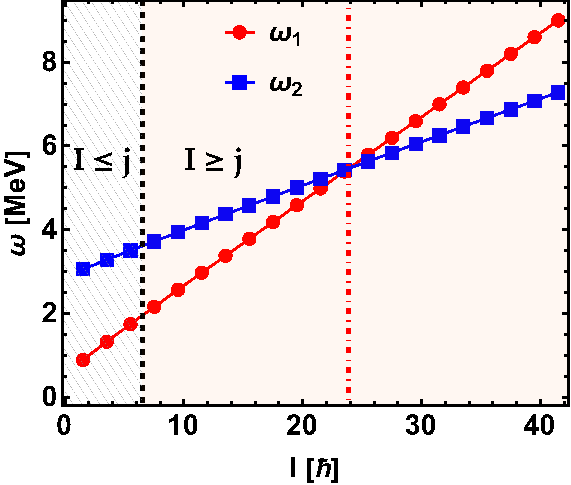
\includegraphics[width=0.47\textwidth]{Chapters/Figures/omega-1-2-frequencies-1.pdf}
    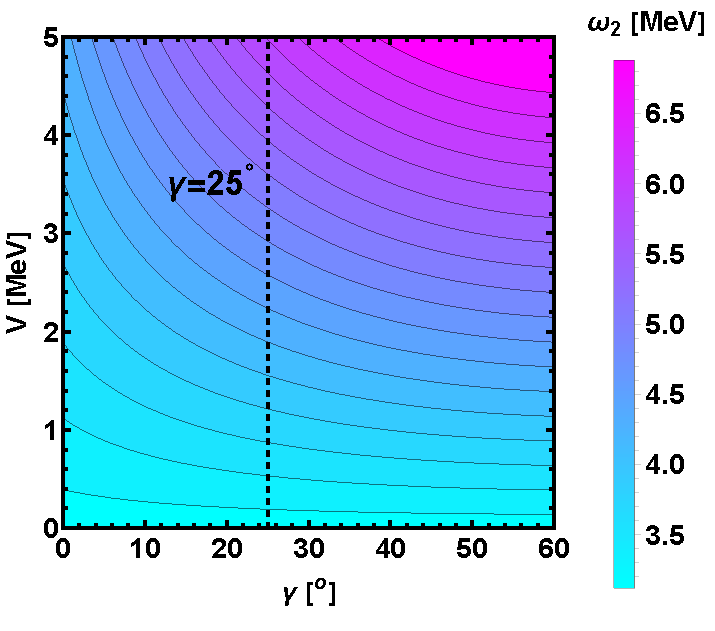
\includegraphics[width=0.49\textwidth]{Chapters/Figures/omega-2-gamma-V.pdf}
    \caption{\textbf{Left:} The oscillator frequencies $\omega_1$ and $\omega_2$ from Eq \ref{small-omega-1-2}. Calculations are given for arbitrary values of the single particle potential $V$, triaxiality parameter $\gamma$ and single-particle $j$-shell. For this particular example, $j=13/2$ and the ordering $A_3>A_2>A_1$ is chosen, according to the conditions of existence for $\omega_1$ and $\omega_2$. The intersection point between $\omega_1$ and $\omega_2$ is marked by the red vertical line around $I\approx 24\hbar$. See text for details on the two colored regions split by the black vertical line. \textbf{Right:} The oscillator frequency $\omega_2$ from Eq. \ref{small-omega-1-2} within the $(\gamma,V)$ plane. Arbitrary values were given for the three inertia factors ($A_3>A_2>A_1$), the total spin, and the single-particle angular momentum. The value of $\gamma=25^\circ$ is marked with the dashed vertical line just to guide the eye. Each contour line represents an energy difference of about $0.20$ MeV.}
    \label{fig-omega1-omega2-cp-omega2}
\end{figure}

Concerning the canonicity factors, they are represented separately in Fig. \ref{fig-k-1-2-factors}. The plots show the evolution of both quantities with respect to the total angular momentum and at different orderings for $A_k$. For the adopted numerical calculations, the values of $A_k$ remained unchanged and only $A_2$ and $A_3$ were reversed. Remarkable the fact that for $k_2$, reversing the factors $A_{2,3}$ will change the behavior with respect to spin from an increasing one ($A_3>A_2$) to a decreasing type ($A_2>A_3$). The same cannot be said about $k_1$, where both orderings give an increasing trend w.r.t. spin. Note that just for a pedagogical purpose, the plots contain the regions where $I\leq j$, similarly as per Fig. \ref{fig-omega1-omega2-cp-omega2}.
\begin{figure}
    \centering
    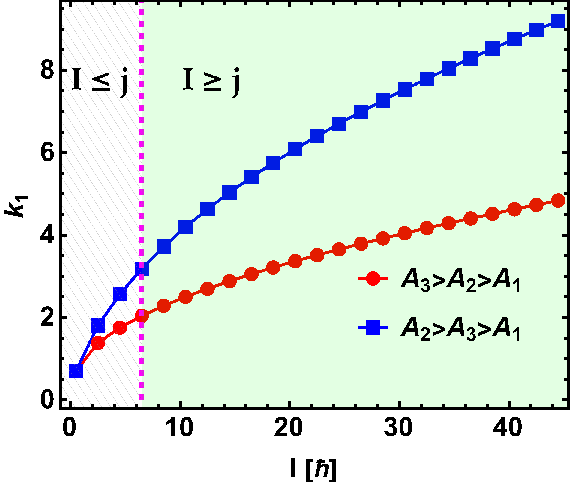
\includegraphics[scale=0.7]{Chapters/Figures/k1_factor.pdf}
    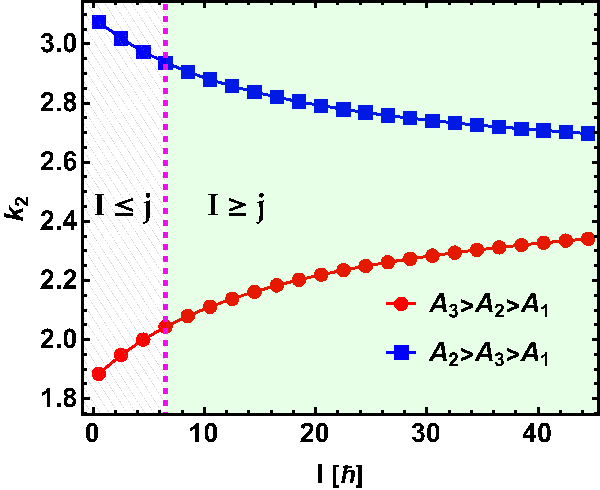
\includegraphics[scale=0.7]{Chapters/Figures/k2_factor.pdf}
    \caption{The canonicity factors defined in Eq. \ref{canonicity-factors} are graphically represented as function of spin $I$ for arbitrary MOI, $V$ and $\gamma$. The single-particle angular momentum is set to $j=13/2$. For the calculations, the two $A_k$ orderings kept the same numerical values and only $A_2$ and $A_3$ were interchanged. The regions where $I\leq j$ (hatched area) and $I\geq j$ (green area) that are split by the vertical dashed line are pointed out as well.}
    \label{fig-k-1-2-factors}
\end{figure}

Since the structure of $k_2$ is dependent on the triaxiality parameter and the single-particle potential strength, a set of contour plots within this plane can also be created, in a similar fashion as the one obtained for $\omega_2$ from Fig. \ref{fig-omega1-omega2-cp-omega2}. For this case though, by reversing $A_2$ and $A_3$ will in fact produce significant changes on the values of $k_2$ (recall Fig. \ref{fig-k-1-2-factors} where the condition $A_2>A_3$ gave decreasing behavior for the canonicity factor). Consequently, two such contour plots are depicted in Fig. \ref{fig-k2-factor-contour}.
\begin{figure}
    \centering
    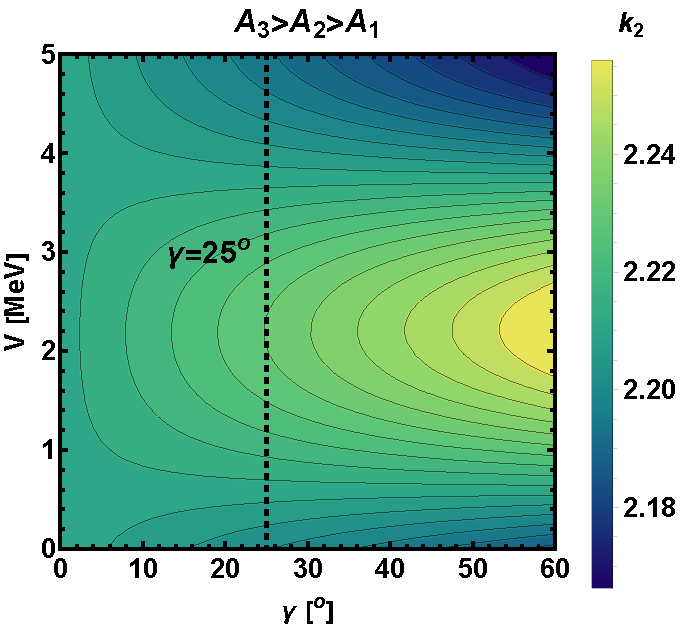
\includegraphics[width=0.49\textwidth]{Chapters/Figures/k2_CP.pdf}
    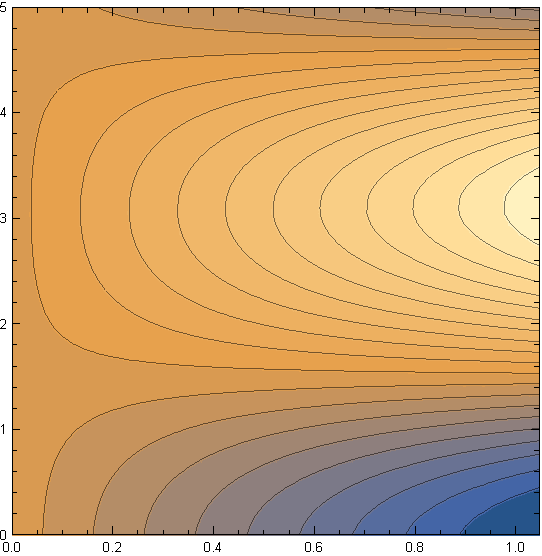
\includegraphics[width=0.5\textwidth]{Chapters/Figures/k2_reversed_CP.pdf}
    \caption{The canonicity factor $k_2$ from Eq. \ref{canonicity-factors} in the ($\gamma,V)$ plane, evaluated at fixed inertia factors and angular momenta. In each figure the terms $A_2$ and $A_3$ have been reversed but the other parameters remained unchanged. The value $\gamma=25^\circ$ is marked by the vertical dashed line just to guide the eye.}
    \label{fig-k2-factor-contour}
\end{figure}

This alternative description for obtaining a set of solutions that describe a harmonic motion of the core $\mathscr{C}$ and the odd single-particle $\mathcal{Q}$ comprised $a)$ the required steps in acquiring analytical results in regards to the energy spectra and $b)$ qualitative analyses for some of the quantities that emerged from calculations. Furthermore, by quantizing the classical variables obtained from TDVE, it is possible to attain a new classical energy function of a triaxial nucleus, which can be summarized in the following way: \emph{The CEF is composed of 1) a term that is independent of any canonical variable and 2) two harmonic vibrators with the phonon energies} $\left\{\Omega_1,\Omega_2\right\}$, \emph{portraying the precessional motion of the core and the odd particle}. The oscillators emerge from the solutions of a fourth degree algebraic equation (Eq. \ref{omega-equation-linearized}), whose origin was deducted in a `quantized manner', i.e., the description shown above (starting with Eq. \ref{canonical-coordinates-quantized}). This is indeed a remarkable feature of the current model, since the dequantization procedure of the initial Hamiltonian and further \emph{re-quantization} of $\mathcal{H}$ can be done consistently without any loss of the underlying system dynamics and degrees of freedom. The final form of the energy spectrum is defined analytically in Eq. \ref{tsd-bands-compressed-spectrum}, where the first term of the expansion of $\mathcal{H}$ around its minimum point is given by $\mathcal{H}_\text{min}^I$ and the two oscillators comprised in $\mathcal{F}_{n_{w_1}n_{w_2}}^I$ (Eq. \ref{phononic-term-tsd-energies}).

Regarding the energy spectrum $E_{I,n_{w_1},n_{w_2}}$ obtained in Eq. \ref{tsd-bands-compressed-spectrum} and Eq. \ref{tsd-bands-general-spectrum}, when both wobbling phonon numbers are zero, it simply reflects the \emph{zero-point-motion} for the system, i.e., the true ground state. Even when $n_{w_1}=n_{w_2}=0$, the core and particle will contribute to the total energy of the system, through the smallest `quantum fluctuations` characterized by $\Omega_1/2$ and $\Omega_2/2$, which is consistent with the harmonic description of the triaxial rigid rotators. This will be crucial when the real wobbling spectrum of the studied nuclei will be interpreted with the current formalism.

\section{A New Band Structure in Lu Isotopes}

Following up to the team's work with regards to the so-called $\mathbf{W_0}$ approach that was outlined in Section \ref{foundation}, two more research papers were devoted to the study of wobbling motion in Lu isotopes (see Refs. \cite{raduta2020approach,raduta2020towards}), but with a different perspective in reference to the band structure. In what follows, the new interpretation (hereafter referred to as $\mathbf{W_1}$) will be described, while also pointing out key distinctions between it and $\mathbf{W_0}$.

Recalling the mechanism that generates the wobbling states via $\mathbf{W_0}$, this was depicted in Fig. \ref{phonon-operator-schematic}, and in this scheme it was shown that from the ground states (calculated variationally according to Eq. \ref{tdve-approach-w1}), one can obtain energy levels for bands $n_w=1, 2, \dots$ by acting with a phonon operator once, twice, and so on, on a given spin state $I$. Moreover, a spin state $I$ from a band $n_w=n'$ emerged by means of the phonon operator which acts on $I-1$ from the band $n_w=n'-1$. The formalism $\mathbf{W_0}$ clearly shows the fact that the variational method can be applied to the ground-band and furthermore get excited bands through an additional term (i.e., the phonon operator), which can be successively applied on ground states. On the other hand, $\mathbf{W_1}$ changes this landscape by aiming at a more \emph{compact} method in attaining the wobbling spectrum. In order to better understand this procedure, a specific case-study for $^{163}$Lu will be employed in the following subsection and a generalization to other isotopes can be inherently adopted going further.

\subsection{Variational States}
\label{subsection-variational-states}

The isotope $^{163}$Lu has been studied successfully by the team within the $\mathbf{W_0}$ and also through the current $\mathbf{W_1}$ model. In both approaches one considered the wobbling spectrum as being composed of four TSD bands. In $\mathbf{W_0}$ the bands were one ground (TSD1) and three excited (TSD2-3-4), which were `in line' with other studies on this isotope \cite{schonwasser2003one,jensen2004coexisting,tanabe2008selection}. The general characteristics of the four triaxial bands and their particle + core structure were already described at the beginning of the chapter from the perspective of $\mathbf{W_0}$. Experimentally, the collective structure of $^{163}$Lu is summarized in Table \ref{lu-163-table-info}.
\begin{table}
    \centering
    \resizebox{\textwidth}{!}{%
    \begin{tabular}{|c|c|c|c|c|c|c|}
    \hline
    Band & Spins & $\pi$ & $\alpha$ & $\mathcal{Q}_p:\ \pi(l_j)$ & $\mathscr{C}:\mathbf{W_0}$ & $\mathscr{C}:\mathbf{W_1}$ \\ \hline
    TSD1 & $13/2,17/2 \dots 97/2$ & $+1$ & $+1/2$ & $\pi(i_{13/2})$ & $0^+,2^+,4^+,\dots$ & $0^+,2^+,4^+,\dots$ \\ \hline
    TSD2 & $27/2,31/2 \dots 91/2$ & $+1$ & $-1/2$ & $\pi(i_{13/2})$ & $\text{TSD1}+1\Gamma^\dagger$ & $1^+,3^+,5^+,\dots$ \\ \hline
    TSD3 & $33/2,37/2 \dots 85/2$ & $+1$ & $+1/2$ & $\pi(i_{13/2})$ & $\text{TSD1}+2\Gamma^\dagger$ & $\text{TSD2}+\Gamma^\dagger$ \\ \hline
    TSD4 & $47/2,51/2 \dots 83/2$ & $-1$ & $-1/2$ & $\pi(h_{9/2})$  & $\text{TSD1}+3\Gamma^\dagger$ & $1^+,3^+,5^+,\dots$ \\ \hline % TSD4 from 163Lu has odd spin states with negative parity
    \end{tabular}%
    }
    \caption{The data concerning spins, parity, and signature assignments for $^{163}$Lu from experimental measurements \cite{reich2010nuclear}. The last two columns represent the key difference between formalisms $\mathbf{W_0}$ and $\mathbf{W_1}$, namely the particle + core coupling. Note that in this new approach, the band TSD3 is the one-phonon band built on top of TSD2. Concerning the notation $\pi(l_j)$, it signifies an odd proton in the $l$-orbital with angular momentum $j$.}
    %The last two columns represent the quasi-particle $\mathcal{Q}$ and the core $\mathscr{C}$ (according to the notations from Table \ref{notation-table-wobbling}) for each TSD band as per $\mathbf{W_0}$. Note that $\mathcal{Q}$ is different for TSD4 and the core angular momentum $\mathscr{C}$ is only defined for TSD1 because the excited bands are created through $\Gamma^\dagger$ phonon operator (see Section \ref{foundation}).}
    \label{lu-163-table-info}
\end{table}

Within the \emph{renormalization} of $\mathbf{W_1}$ for the nucleus $^{163}$Lu, one applies the variational principle (i.e., Eq. \ref{tdve-approach-w1}) for all states in TSD1 and TSD2. Additionally, since the coupling scheme $\mathcal{Q}+\mathscr{C}$ is different for TSD4 (i.e., the $j=9/2$ proton couples with the even-even core as opposed to the $j=13/2$ proton for the other bands), then another VP will be employed for TSD4 as well. The states from TSD3 emerge as excited wobbling states that are formed by the action of a phonon operator on TSD2. Indeed, this \emph{successive application of TDVE in obtaining variational states is a remarking aspect of} $\mathbf{W_1}$.

All the states from TSD1 are produced by coupling the $j=13/2$ odd proton from $i$-shell with a triaxial even-even core having the spin sequence $\mathscr{C}_1=0,2,4,\dots$, forming a zero-phonon wobbling band. Both the core and the single-particle have positive parity. On the other hand, all states in TSD2 are built by the same odd-particle, but with a different \emph{core}: $\mathscr{C}_2=1,3,5\dots$, which also has positive parity. Notice the even/odd dissimilarity between the two angular momentum sequences of the cores $\mathscr{C}_1$ and $\mathscr{C}_2$ that are specified in Table \ref{lu-163-table-info} and compared to the previous $\mathbf{W_0}$ theory. The wobbling bands TSD1 and TSD2 from $^{163}$Lu can be explained by means of a semi-classical model through an even-odd staggering of states $(0^+,1^+),\ (2^+,3^+),\ \dots$ of collective nature. They are in fact \emph{Signature Partner Bands} \cite{raduta2020approach}: two sequences of states that differ with $\Delta I=2\hbar$ inside the bands and $\Delta I=1\hbar$ for adjacent spins, each having opposite signature but similar parity. In Ref. \cite{raduta2020towards} it was proven that TSD2 is the signature partner of TSD1 because the potential well is deep enough such that the second band does not exhibit secondary minima. The negative parity states belonging to the band TSD4 can be explored semi-classically via TDVE with the collective core $\mathscr{C}_2=1,3,5\dots$ coupled to a negative parity proton $j^\pi=9/2^-$. Recall that the signature quantum number was described in Chapter \ref{chapter-3} (Section \ref{section-ral-signature}) and its definition is given in Eq. \ref{signature-quantum-number}.

In terms of quasi-particle + triaxial core coupling, it is remarkable the fact that the `final picture' for $^{163}$Lu is regarded as a positive parity core of even spin states that generates the band TSD1 (i.e., $\mathscr{C}_1$), a core with odd spin states of positive parity states forming TSD2 and TSD4 (i.e., $\mathscr{C}_2$), and finally the one-phonon states in TSD3, which are activated from the ground band TSD2. This is emphasized within the last two columns of Table \ref{lu-163-table-info}. One can encapsulate this current renormalization under the following set of \emph{equalities}:
\begin{align}
    \{TSD1\}&\equiv\left\{\mathscr{C}_1\left[0^+,2^+,4^+,\dots\right] \otimes \mathcal{Q}_1[j^\pi=13/2^+]\right\}\ ,\ \nonumber\\
    \{TSD2\}&\equiv\left\{\mathscr{C}_2\left[1^+,3^+,5^+,\dots\right] \otimes \mathcal{Q}_1[j^\pi=13/2^+]\right\}\ ,\ \nonumber\\
    \{TSD4\}&\equiv\left\{\mathscr{C}_2\left[1^+,3^+,5^+,\dots\right] \otimes \mathcal{Q}_2[j^\pi=9/2^-]\right\}\ ,
    \label{renormalized-bands-structure-TSD124}
\end{align}
for TSD1-2-4 and:
\begin{align}
    \{TSD3\left[\dots,I^+,(I+2)^+,\dots\right]\}\equiv\left\{TSD2\left[\dots,(I-1)^+,(I+1)^+,\dots\right]+\Gamma^\dagger\right\}\ ,
    \label{renormalized-bands-structure-TSD3}
\end{align}
for TSD3. The two odd protons from Table \ref{lu-163-phonon-numbers} are denoted with $\mathcal{Q}_1$ and $\mathcal{Q}_2$ in Eqs. \ref{renormalized-bands-structure-TSD124} - \ref{renormalized-bands-structure-TSD3}, and these notations will be used hereafter. Thus, the two equations make up the renormalization of $\mathbf{W_1}$, which is successfully applied not only to $^{163}$Lu but also to other isotopes.% and their angular momenta will be labelled $j_1=13/2$ for $\mathcal{Q}_1$ and $j_2=9/2$ for $\mathcal{Q}_2$. The $p$-abbreviation from the quasi-particle notation (as per the rules in Table \ref{notation-table-wobbling}) will be dismissed from now on because all the discussed isotopes have odd the odd nucleon with \emph{particle} character. The labelling for both $\mathcal{Q}_1$ and $\mathcal{Q}_2$ is given in Table \ref{lu-163-phonon-numbers}.

With the Eqs. \ref{renormalized-bands-structure-TSD124} - \ref{renormalized-bands-structure-TSD3} as `recipes', one can obtain the wobbling energies for this isotope as per Eq. \ref{tsd-bands-general-spectrum}, by adopting the spin values $I$ and the wobbling phonon numbers $n_{w_1}$ and $n_{w_2}$ of each band in particular. These values are given in Table \ref{lu-163-phonon-numbers}. Notice that for TSD1-2-4 the pair of phonon numbers are $(0,0)$ due to them being variational ground states. Moreover, the TSD3 states are activated only by the wobbling-phonon number $n_{w_1}$ (i.e., $n_{w_2}=0$), which is consistent with the theory from $\mathbf{W_0}$. As it will be seen, all four bands have the wobbling frequency $\Omega_2$ in the zero-point energy, that is $\frac{1}{2}\Omega_2^I$. In reference to TSD3, given that the band is obtained as one-phonon excitations built on top of TSD2, then by acting with the operator on a state $I$ from TSD2 it will increase the angular momentum by one unit (see Fig. \ref{phonon-operator-schematic} from Section \ref{foundation}). Consequently, for a state $I\in\{\text{TSD3}\}$ the phonon operator is indeed $\mathcal{F}_{10}^{I-1}$, where the state $I-1$ belongs in TSD2.
\begin{table}
    \centering
    \resizebox{\textwidth}{!}{%
    \begin{tabular}{|c|c|c|c|c|c|c|}
    \hline
    Bands & $n_{w_1}$ & $n_{w_2}$ & $\mathcal{F}_{n_{w_1}n_{w_2}}^I$ & $I_0$    & $I_t$    & $\mathcal{Q}$    \\ \hline
    TSD1  & $0$       & $0$       & $\mathcal{F}_{00}^I=\frac{1}{2}\left(\Omega_1^I+\Omega_2^I\right)$ & $13/2^+$ & $97/2^+$ & $j^\pi=13/2^+\stackrel{not}{\equiv}\mathcal{Q}_1$ \\ \hline
    TSD2  & $0$       & $0$       & $\mathcal{F}_{00}^I=\frac{1}{2}\left(\Omega_1^I+\Omega_2^I\right)$ & $27/2^+$ & $91/2^+$ & $j^\pi=13/2^+\stackrel{not}{\equiv}\mathcal{Q}_1$ \\ \hline
    TSD3  & $1$       & $0$       & $\mathcal{F}_{10}^{I-1}=\frac{3}{2}\Omega_1^{I-1}+\frac{1}{2}\Omega_2^{I-1}$ & $33/2^+$ & $85/2^+$ & $j^\pi=13/2^+\stackrel{not}{\equiv}\mathcal{Q}_1$ \\ \hline
    TSD4  & $0$       & $0$       & $\mathcal{F}_{00}^I=\frac{1}{2}\left(\Omega_1^I+\Omega_2^I\right)$ & $47/2^-$ & $83/2^-$ & $j^\pi=9/2^-\stackrel{not}{\equiv}\mathcal{Q}_2$  \\ \hline
    \end{tabular}%
    }
    \caption{The wobbling phonon numbers of $^{163}$Lu that correspond to the phonon frequencies $\Omega_1$ and $\Omega_2$, respectively (see Eq. \ref{phononic-term-tsd-energies}). For completeness the first ($I_0$) and last ($I_t$ for \emph{terminus}) spin states of each band are given. The quasi-particles involved in the particle + rotor coupling are denoted according to Eqs. \ref{renormalized-bands-structure-TSD124} - \ref{renormalized-bands-structure-TSD3}. See text for the $\mathcal{F}_{10}^{I-1}$ term.}
    \label{lu-163-phonon-numbers}
\end{table}

Taking the information comprised in Table \ref{lu-163-phonon-numbers} in order to compute the phonon terms (Eq. \ref{phononic-term-tsd-energies}) and by using the general energy formula obtained in Eq. \ref{tsd-bands-general-spectrum}, one can determine the wobbling spectrum of $^{163}$Lu through the following set of equations:
\begin{align}
    E_{I,0,0}^\text{TSD1}=&\epsilon_{13/2}+\mathcal{H}_\text{min}^I+\mathcal{F}_{00}^I=\epsilon_{13/2}+\mathcal{H}_\text{min}^I+\frac{1}{2}\left(\Omega_1^I+\Omega_2^I\right)\ ,\nonumber\\
    E_{I,0,0}^\text{TSD2}=&\epsilon_{13/2}+\mathcal{H}_\text{min}^I+\mathcal{F}_{00}^I=\epsilon_{13/2}+\mathcal{H}_\text{min}^I+\frac{1}{2}\left(\Omega_1^I+\Omega_2^I\right)\ ,\nonumber\\
    E_{I,1,0}^\text{TSD3}=&\epsilon_{13/2}+\mathcal{H}_\text{min}^{I-1}+\mathcal{F}_{10}^{I-1}=\epsilon_{13/2}+\mathcal{H}_\text{min}^{I-1}+\frac{1}{2}\left(3\cdot\Omega_1^{I-1}+\Omega_2^{I-1}\right)\ ,\nonumber\\
    E_{I,0,0}^\text{TSD4}=&\epsilon_{9/2}+\mathcal{H}_\text{min}^{I}+\mathcal{F}_{00}^{I}=\epsilon_{9/2}+\mathcal{H}_\text{min}^{I}+\frac{1}{2}\left(\Omega_1^{I}+\Omega_2^{I}\right)\ ,
    \label{lu163-absolute-energies-tsd1234}
\end{align}
where $\epsilon_{13/2}$ and $\epsilon_{9/2}$ are the single-particle shell energies for $\mathcal{Q}_1$ and $\mathcal{Q}_2$, respectively. For each band, the spins are the ones from Table \ref{lu-163-table-info}. Keep in mind that the wobbling frequencies and the minimal energy both depend on the single-particle angular momentum $j$ as well, so it must be properly inserted for each band as per Table \ref{lu-163-phonon-numbers}. 
% An alternative way of depicting the energy from TSD3 is through the formula:
% \begin{align}
%     E_{I,1,0}^\text{TSD3}=E_{I-1,0,0}^\text{TSD2}+\Omega_1^{I-1}\ .\nonumber
% \end{align}

The obtained set of formulas given in Eq. \ref{lu163-absolute-energies-tsd1234} represents the \emph{absolute values} for the energies. As such, they will be subtracted from the band-head energy of $^{163}$Lu, obtaining thus the spectrum of \emph{excitation energies} (recall Eq. \ref{excitation-energy-general-formula}). The band-head energy $E_{13/2,0,0}^\text{TSD1}$ is the energy corresponding to the ground-state $I_b=13/2$ from TSD1. Its expression is as follows:
\begin{align}
    E_{13/2,0,0}^\text{TSD1}=\epsilon_{13/2}+\mathcal{H}_\text{min}^{13/2}+\mathcal{F}_{00}^{13/2}=\epsilon_{13/2}+\mathcal{H}_\text{min}^{13/2}+\frac{1}{2}\left(\Omega_1^{13/2}+\Omega_2^{13/2}\right)\ .
    \label{lu163-absolute-energy-band-head}
\end{align}

An important aspect of working with the excitation energies within the numerical computations is that the single-particle energies will practically cancel out. Only for TSD4 there will be the constant term $\epsilon_{9/2}-\epsilon_{13/2}=-0.344$ MeV \cite{raduta2020towards}, which is just the difference between the two spherical shell model states of $\mathcal{Q}_2$ and $\mathcal{Q}_1$. Regarding the two wobbling frequencies, in the case of $^{163}$Lu their expressions are:
\begin{align}
    \Omega_{1,2}=\left[\frac{1}{2}\left(-B\mp\sqrt{B^2-4C}\right)\right]^{1/2}\ ,
    \label{wobbling-frequencies-Omega-1-2}
\end{align}
such that the ordering $\Omega_1<\Omega_2$ holds true. The minimal energy term $\mathcal{H}_\text{min}^I$, which firstly appeared in Eq. \ref{tsd-bands-compressed-spectrum} has the structure \cite{poenaru2021extensive1}:
\begin{align}
    \mathcal{H}_\text{min}^I=\left(A_2+A_3\right)\frac{I+j}{2}+A_1(I-j)^2-V\frac{2j-1}{j+1}\sin\left(\gamma+\frac{\pi}{6}\right)\ .
    \label{minimal-energy-term-hmin}
\end{align}

\subsection{Fitting Parameters}

With the help of Eq. \ref{lu163-absolute-energies-tsd1234}, a compact analytical structure for the wobbling spectrum of $^{163}$Lu is obtained within the $\mathbf{W_1}$ formalism. Additionally, the base rule in calculating the excitation energies (by the subtraction of Eq. \ref{lu163-absolute-energy-band-head} from each level) gives the primary step in the fitting procedure. As for the components that comprise the formula of the energy itself, the term $\mathcal{H}_\text{min}^I$ is adopted out of Eq. \ref{minimal-energy-term-hmin} and the wobbling frequencies $\Omega_{1,2}$ are taken from Eq. \ref{wobbling-frequencies-Omega-1-2}. 

In order to get numerical results for the excitation energies, a set of free parameters will be employed in the fitting method, such that by fixing these values, the theoretical data are achieved. From the structure of the classical energy function (or even the initial quantal Hamiltonian) it can be seen that the rotational term is expressed in terms of the inertia factors $A_k$ and the single-particle term is explicitly specified through the single-particle strength $V$ and triaxiality $\gamma$. Therefore, it is well suited to pick the following quantities as fitting parameters throughout the numerical computations:
\begin{enumerate}
    \item moments of inertia: $\mathcal{I}_1$, $\mathcal{I}_2$, $\mathcal{I}_3$
    \item single-particle potential strength $V$
    \item triaxiality parameter $\gamma$
\end{enumerate}
whose values will be denoted as:
\begin{align}
    \mathcal{P}_\text{fit}=\left[\mathcal{I}_1,\mathcal{I}_2,\mathcal{I}_3,V,\gamma\right]\ .
    \label{fitting-parameters-p-fit}
\end{align}

The actual fitting technique consists of finding the set $\mathcal{P}_\text{fit}$ that best reproduces the experimental data concerning the wobbling spectrum. The numerical implementation aims at determining $\mathcal{P}_\text{fit}$ such that the $\chi^2$-function \cite{poenaru2021extensive1} :
\begin{align}
    \chi^2=\frac{1}{N_T}\sum_i\frac{\left(E_\text{exp}^{(i)}-E_\text{th}^{(i)}\right)^2}{E_\text{exp}^{(i)}}\ ,
    \label{chi-2-fitting-function}
\end{align}
is \emph{minimal}. Here $N_T$ represents the total number of states for the isotope. In the case of $^{163}$Lu, the $\chi^2$-function will contain all states belonging to TSD1-2-3 and TSD4. Obviously $E_\text{exp}^{(i)}$ represents the \emph{experimental excitation energy}, which is evaluated by subtracting the band-head level (having an energy of $1.738\ \text{MeV}$) from each state. From a computational standpoint, the problem thereby consists of a minimization process that has to be tackled on the $\chi^2$-function.

This new approach is different than $\mathbf{W_0}$ in the sense that the moments of inertia are now considered as separate (independent) `free' values, whereas in \cite{raduta2017semiclassical} one of the parameters was the scaling factor $1/\mathcal{I}_0$ emerging from the adoption of the rigid-body MOI (see Eq. \ref{eq-irrotational-rigid-mois}). Moreover, in the present model the three moments of inertia have no angular momentum dependence, i.e., they are fixed and remain constant across the entire spin range of each isotope. On the other side, unlike $\mathbf{W_0}$ where $\gamma$ and $\beta$ were fixed with values from literature, this re-interpretation obtains $\gamma$ self-consistently right from the fitting procedure. Both approaches consider $V$ as a free parameter, and its value is obtained from the minimization of the $\chi^2$-function.

The strong argument in using a set of free MOI is related to the fact that the \emph{real} moments of inertia for the nucleus are neither irrotational nor rigid, but they satisfy the relation $\mathcal{I}^\text{irr}<\mathcal{I}^\text{exp}<\mathcal{I}^\text{rig}$ (recall discussion in Chapter \ref{chapter-3} and Eq. \ref{experimental-MOI-vs-rig-irr}). A study of the three moments of inertia in regards to a possible change in magnitude at higher spins due to Coriolis or even pairing interaction is excluded within this technique as the initial quantal Hamiltonian does not contain such terms. Lastly, the $\beta_2$ quadrupole deformation parameter does not appear explicitly throughout the description since it is somewhat \emph{encoded} in the potential strength $V$ (see Eqs. \ref{quadrupole-deformed-potential-beta} and \ref{quadrupole-deformed-potential-V}). Concluding, the quality of the fitting procedures applied to each isotope will reflect the deformation of the nuclei (i.e., degree of triaxiality and prolate/oblate shape).

\section{Numerical Results in Lu Isotopes}

In the previous section, one formulated: i) the renormalization procedure that is the cornerstone in the $\mathbf{W_1}$ formalism via Eqs. \ref{renormalized-bands-structure-TSD124} - \ref{renormalized-bands-structure-TSD3} ii) a set of analytical expressions of the wobbling bands for $^{163}$Lu provided by Eq. \ref{lu163-absolute-energies-tsd1234} iii) the relevant free parameter set $\mathcal{P}_\text{fit}$ via Eq. \ref{fitting-parameters-p-fit} and finally iv) the actual fitting procedure that will be employed as application (minimization of $\chi^2$ from Eq. \ref{chi-2-fitting-function}). The team's work with the $\mathbf{W_1}$ formalism concluded in two research papers, where in addition to the study of the wobbling properties in $^{163}$Lu \cite{raduta2020towards}, several other Lu isotopes were examined \cite{raduta2020approach}. Herein, the results obtained for $^{161,163,165,167}$Lu will be presented, providing data for quantities like:
\begin{enumerate}
    \item excitation energies
    \item alignments
    \item dynamic moments of inertia
    \item energies relative to a reference rotor
\end{enumerate}

Naturally, calculations concerning the transition probabilities for every nucleus will also be provided, making a comparison with the available experimental data. The first step is to numerically reproduce the general spectrum depicted in Eq. \ref{tsd-bands-general-spectrum}. This is realized by following the rules that were outlined for $^{163}$Lu in Eqs. \ref{lu163-absolute-energies-tsd1234} - \ref{chi-2-fitting-function} and apply them to all of the isotopes. However, a prior knowledge of the two wobbling phonon numbers, the quasi-particle + core coupling scheme, and the spin + parity assignments of each wobbling band is required. The $\mathbf{W_1}$ model considers TSD1 and TSD2 from $^{163}$Lu as being ground-states obtained variationally by coupling an odd particle with two different cores (recall $\mathscr{C}_1$ and $\mathscr{C}_2$ defined in Eqs. \ref{renormalized-bands-structure-TSD124} - \ref{renormalized-bands-structure-TSD3}). A remarking feature of this theory is that the same principle can be used to the other isotopes: namely the pair $(\text{TSD1},\text{TSD2})$ is regarded as zero-phonon bands, which originate from different core + particle couplings. Furthermore, some fitting requirements should be taken into account for every isotope in order to have consistency throughout the numerical implementations performed to the group of nuclides. These can be summarized in the following way:
\begin{itemize}
    \item $^{161}$Lu
    \begin{itemize}
        \item There are only two bands generated by the coupling of $\mathcal{Q}_1$ with an even-even core
        \item In regards to their nature, both bands are ground-states (zero-phonon)
        \item The core in TSD1 has even spins (i.e., $\mathscr{C}_1$) and in TSD2 it has odd spin spins (i.e., $\mathscr{C}_2$)
    \end{itemize}
    \item $^{163}$Lu
    \begin{itemize}
        \item Four TSD bands with the structure described in Table \ref{lu-163-table-info}
        \item Three different core + odd-particle couplings: $(\mathcal{Q}_1+\mathscr{C}_1)\ \to\ \text{TSD1}$, $(\mathcal{Q}_1+\mathscr{C}_2)\ \to\ \text{TSD2}$, and $(\mathcal{Q}_2+\mathscr{C}_1)\ \to\ \text{TSD4}$
    \end{itemize}
    \item $^{165}$Lu
    \begin{itemize}
        \item The three TSD bands are created from a single quasi-particle (i.e., the proton $\mathcal{Q}_1$), which couples to a core of even states (TSD1) and a core with odd states (TSD2).
        \item TSD1-2 are ground-bands
        \item TSD3 is a one-phonon band that is obtained as wobbling excitations built on top of TSD2
    \end{itemize}
    \item $^{167}$Lu
    \begin{itemize}
        \item treated in a similar fashion as the $^{161}$Lu isotope
    \end{itemize}
\end{itemize}

The characteristics of each isotope mentioned above are condensed into a set of tables where, for the sake of completeness, the spin and parity data are indicated. These are sketched in Tables \ref{lu-161-experimental-data-table} - \ref{lu-167-experimental-data-table}. Since the previous section contains the relevant data for $^{163}$Lu (recall Tables \ref{lu-163-table-info} and \ref{lu-163-phonon-numbers}), it has been omitted here. It is worth to point out that besides the fourth TSD band from $^{163}$Lu, every nucleus has wobbling excitations emerging from the coupling of the $\mathcal{Q}_1$ single-particle with an even-even core (containing either even or odd spin states). Indeed, the coupling in TSD4 is between the negative parity proton $\mathcal{Q}_2$ and the positive parity core $\mathscr{C}_1$.
\begin{table}
    \centering
    \resizebox{\textwidth}{!}{%
    \begin{tabular}{|c|c|c|c|c|c|}
    \hline
    Band & Spins                        & $\mathcal{Q}$ & $\mathscr{C}$  & $(n_{w_1},n_{w_2})$ & $I_b$                   \\ \hline
    TSD1 & $21/2^+,25/2^+,\dots,89/2^+$ & $j^\pi=13/2^+$  & $4^+,6^+,8^+\dots$   & $(0,0)$             & \multirow{2}{*}{$21/2$} \\ \cline{1-5}
    TSD2 & $31/2^+,35/2^+,\dots,79/2^+$ & $j^\pi=13/2^+$  & $9^+,11^+,13^+\dots$ & $(0,0)$             &                         \\ \hline
    \end{tabular}%
    }
    \caption{The data concerning spin and parity assignments of $^{161}$Lu that are required for evaluating the excitation energies. The wobbling phonon numbers from Eq. \ref{phononic-term-tsd-energies} are shown in the penultimate column. For both bands there is only one single-particle, i.e., $\mathcal{Q}_1$. The even/odd dissimilarity between core states of the two bands are emphasized through the fourth column ($\mathscr{C}$). The band-head $I_b$ for the isotope is also given in the last column.}
    \label{lu-161-experimental-data-table}
\end{table}
\begin{table}
    \centering
    \resizebox{\textwidth}{!}{%
    \begin{tabular}{|c|c|c|c|c|c|}
    \hline
    Band & Spins                        & $\mathcal{Q}$ & $\mathscr{C}$         & $(n_{w_1},n_{w_2})$ & $I_b$                   \\ \hline
    TSD1 & $25/2^+,29/2^+,\dots,89/2^+$ & $j^\pi=13/2^+$  & $6^+,8^+,10^+\dots$   & $(0,0)$             & \multirow{3}{*}{$25/2$} \\ \cline{1-5}
    TSD2 & $35/2^+,39/2^+,\dots,91/2^+$ & $j^\pi=13/2^+$  & $11^+,13^+,15^+\dots$ & $(0,0)$             &                         \\ \cline{1-5}
    TSD3 & $41/2^+,45/2^+,\dots,81/2^+$ & $j^\pi=13/2^+$  & $\text{TSD2}+\Gamma^\dagger$ & $(1,0)$             &                         \\ \hline
    \end{tabular}%
    }
    \caption{The data concerning spin and parity assignments of $^{165}$Lu that are required for evaluating the excitation energies. The wobbling phonon numbers from Eq. \ref{phononic-term-tsd-energies} are shown in the penultimate column. For all three TSD bands there is only one single-particle, i.e., $\mathcal{Q}_1$. The even/odd dissimilarity between core states of the two bands are emphasized through the fourth column ($\mathscr{C}$). The band-head $I_b$ for the isotope is also given in the last column.}
    \label{lu-165-experimental-data-table}
\end{table}
\begin{table}
    \centering
    \resizebox{\textwidth}{!}{%
    \begin{tabular}{|c|c|c|c|c|c|}
    \hline
    Band & Spins                        & $\mathcal{Q}$ & $\mathscr{C}$         & $(n_{w_1},n_{w_2})$ & $I_b$                   \\ \hline
    TSD1 & $25/2^+,29/2^+,\dots,89/2^+$ & $j^\pi=13/2^+$  & $6^+,8^+,10^+\dots$   & $(0,0)$             & \multirow{2}{*}{$25/2$} \\ \cline{1-5}
    TSD2 & $35/2^+,39/2^+,\dots,91/2^+$ & $j^\pi=13/2^+$  & $11^+,13^+,15^+\dots$ & $(0,0)$             &                         \\ \hline
    \end{tabular}%
    }
    \caption{The data concerning spin and parity assignments of $^{167}$Lu that are required for evaluating the excitation energies. The wobbling phonon numbers (from Eq. \ref{phononic-term-tsd-energies}) are shown in the penultimate column. For both bands, there is only one single-particle, i.e., $\mathcal{Q}_1$. The even/odd dissimilarity between core states of the two bands are emphasized through the fourth column ($\mathscr{C}$). The band-head $I_b$ for the isotope is also given in the last column.}
    \label{lu-167-experimental-data-table}
\end{table}

Putting together the set of absolute energies from Eq. \ref{lu163-absolute-energies-tsd1234} and the discussion in reference to the excitation energy for a state $I$, one can define a general formula that will illustrate the systematics of the wobbling states to be used within the fitting procedure:
\begin{align}
    E_{I_b}^\text{TSD1}(^A\text{Lu\ ;\ abs})=&\epsilon_{13/2}+\mathcal{H}_\text{min}^{I_b}+\mathcal{F}_{00}^{I_b}\ ,\label{absolute-energy-fitting-model}\\
    E_{I,n_{w_1},n_{w_2}}^{\text{TSD}N}(^A\text{Lu\ ;\ exc})=&\left(\epsilon_{j}+\mathcal{H}_\text{min}^I+\mathcal{F}^I_{n_{w_1}n_{w_2}}\right)-E_{I_b}^\text{TSD1}(^A\text{Lu\ ;\ abs})\ ,
    \label{general-excitation-energy-fitting-model}
\end{align}
where $^A$Lu represents the isotope that is evaluated (i.e., $A\in\{161,163,165,167\}$), $I$ is the state belonging to a triaxial band $N$ from $^A$Lu ($I\in\text{TSD}N\ ,\ I>I_b$), and the labels `$\text{abs}$/$\text{exc}$' symbolize the absolute/excitation energy, respectively. Additionally, $I_b$ is the band-head of the corresponding nucleus, and it is given explicitly in the last column of Tables \ref{lu-161-experimental-data-table} - \ref{lu-167-experimental-data-table}. The value $\epsilon_j$ denotes the single-particle proton's energy for either $j=13/2$ ($\mathcal{Q}_1$) or $j=9/2$ ($\mathcal{Q}_2$). The energy from Eq. \ref{absolute-energy-fitting-model} corresponds to the absolute energy of the band-head, which was firstly depicted for $^{163}$Lu in Eq. \ref{lu163-absolute-energy-band-head}. For simplicity, the subscripts $n_{w_1}$ and $n_{w_2}$ appearing in $E_{I_b}^\text{TSD1}(^A\text{Lu\ ;\ abs})$ have been dropped entirely because TSD1 has $n_{w_1}=n_{w_2}=0$. It can be seen now that by using Eq. \ref{general-excitation-energy-fitting-model} the single-particle energy for bands TSD1-3 simply vanish, while only for TSD4 in $^{163}$Lu the quantity $\epsilon_{9/2}-\epsilon_{13/2}$ shows up.
%Moreover, the quasi-particle involved in the particle + rotor coupling for the ground bands is $\mathcal{Q}_1$ across the entire mass region.
% reference for Q1 and Q2 particle notations (Table \ref{lu-163-phonon-numbers})

Concluding the current section, Eq. \ref{general-excitation-energy-fitting-model} provides the final ingredient towards the determination of the energy spectra for the whole group of nuclides. Indeed, the $\chi^2$-function can be minimized using $E_{I,n_{w_1},n_{w_2}}^{\text{TSD}N}(^A\text{Lu\ ;\ exc})$ as the model and the data collected in Tables \ref{lu-161-experimental-data-table} - \ref{lu-167-experimental-data-table} will be adopted as input. The full workflow is depicted in Fig. \ref{fitting-workflow-fig}.
\begin{figure}
    \centering
    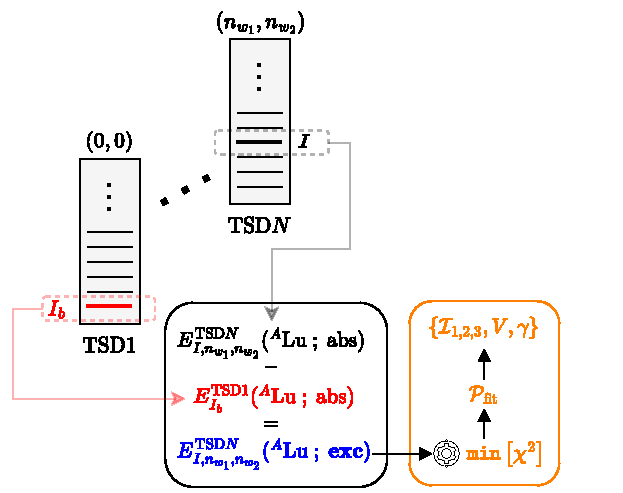
\includegraphics[width=0.99\textwidth]{Chapters/Figures/fitting_procedure_chi2.pdf}
    \caption{A schematic representation showing the overall workflow of solving the minimization of $\chi^2$-function (Eq. \ref{chi-2-fitting-function}). Initially, the absolute energy of the band-head $I_b$ (Eq. \ref{absolute-energy-fitting-model} - red color) is subtracted from every state $I$ (Eq. \ref{tsd-bands-compressed-spectrum}) in order to obtain the excitation energy (Eq. \ref{general-excitation-energy-fitting-model} blue color). This is applied for every state within all of the isotope's bands. Next, the inputs from Tables \ref{lu-163-table-info} - \ref{lu-167-experimental-data-table} are used in the minimization of $\chi^2$. The fitting function returns the set of parameters $\mathcal{P}_\text{fit}$ (Eq. \ref{fitting-parameters-p-fit}) that best reproduce the experimental results.}
    \label{fitting-workflow-fig}
\end{figure}

\subsection{Numerical Parameters}

With the theoretical and experimental excitation energies attributed to each nucleus, the minimization procedure of Eq. \ref{chi-2-fitting-function} can be readily applied. Note that since the variational states from TSD4 are obtained from a different core + particle polarization, a separate fit for the states of this band will be made \cite{raduta2020towards}. Results are presented in Table \ref{numerical-fitting-parameters-Lu-isotopes}, where in order to appraise the quality of the fits, the root-mean-square (RMS) error \cite{kenney1939mathematics} for all bands is also shown. Based on the obtained statistic, it can be concluded that the description of the excitation energies is quite good across the entire mass region.
\begin{table}
    \centering
    \resizebox{\textwidth}{!}{%
    \begin{tabular}{ccccccccc}
    \hline
    \hline
    Isotope &  Bands & $\mathcal{I}_1$ $\left[\hbar^2/\text{MeV}\right]$ & $\mathcal{I}_2$ $\left[\hbar^2/\text{MeV}\right]$ & $\mathcal{I}_3$ $\left[\hbar^2/\text{MeV}\right]$ & $V$ [MeV] & $\gamma$ [$^\circ$] & n.o.s & $E_\text{rms}$ [MeV] \\ \hline
    $^{161}$Lu & TSD1-2 & 87.555 & 2.773  & 22.744 & 2.933 & 20    & 29 & 0.168 \\
    $^{163}$Lu & TSD1-3 & 63.2   & 20     & 10     & 3.1   & 17    & 52 & 0.264 \\
               & TSD4   & 67     & 34.5   & 50     & 0.7   & 17    & 10 & 0.057 \\
    $^{165}$Lu & TSD1-3 & 77.295 & 16.184 & 4.399  & 1.673 & 20    & 42 & 0.125 \\
    $^{167}$Lu & TSD1-2 & 87.032 & 10.895 & 3.758  & 8.167 & 19.48 & 30 & 0.165 \\
     \hline
     \hline
    \end{tabular}%
    }
    \caption{The fitting parameters $\mathcal{P}_\text{fit}$, i.e., the moments of inertia, the single-particle potential strength, and the triaxiality $\gamma$ for each Lu isotope. Numerical results were achieved via the fitting procedure described in text. The number of wobbling states and the root-mean-square error are also given in the last two columns.}
    \label{numerical-fitting-parameters-Lu-isotopes}
\end{table}

To evidentiate the dependence of the three MOI with respect to the atomic mass $A$, the numerical values of $\mathcal{I}_k$ from Table \ref{numerical-fitting-parameters-Lu-isotopes} are graphically represented in Fig. \ref{MOIs-A-behavior-Lu-isotopes}, where one remarks a change in their ordering at $A=163$. Such a change can be regarded as a \emph{phase transition}. Moreover, there is a similar ordering concerning $\mathcal{I}_2$ and $\mathcal{I}_3$ between $^{161}$Lu and TSD4 from $^{163}$Lu, while the same order is reversed for the other nuclides.
\begin{figure}
    \centering
    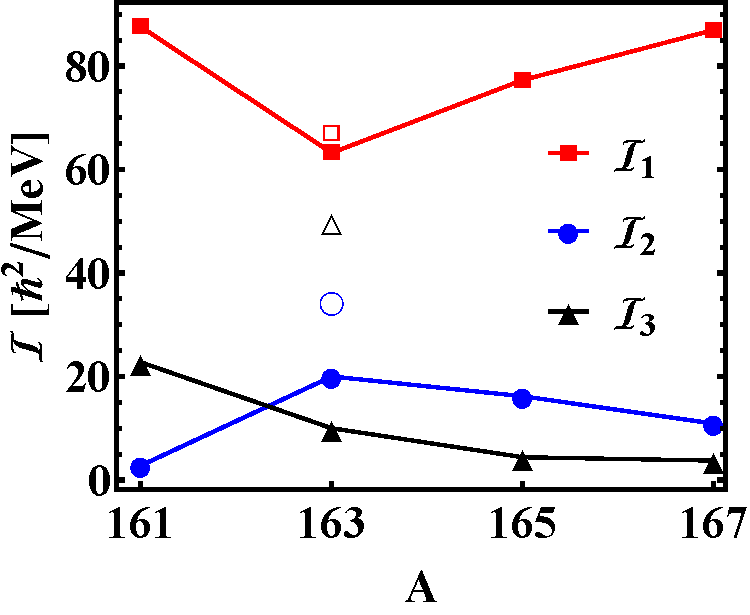
\includegraphics[scale=0.65]{Chapters/Figures/fig1_moivalues.pdf}
    \caption{The fitted MOI from Table \ref{numerical-fitting-parameters-Lu-isotopes} plotted as a function of the mass number $A$. The unfilled symbols represent the band TSD4 of $^{163}$Lu.}
    \label{MOIs-A-behavior-Lu-isotopes}
\end{figure}

From the obtained MOI, one sees that the maximal value is corresponding to $1$-axis. As per the discussion regarding wobbling regime from Chapter \ref{chapter-5}, the interaction of the core with the odd particle seems to drive the system to a longitudinal-like motion. However, in the `final picture', one is unable to assert that these isotopes behave as transverse or longitudinal wobblers. This is due to the fact that within the current model, the MOI do not have angular momentum dependence, and it is impossible to pinpoint regions across the range of $I$ where transitions from transverse to longitudinal wobbling might occur. Certainly, it could be that at low rotational motion the ordering is $\mathcal{I}_2>\mathcal{I}_1>\mathcal{I}_3$ and then gradually shift to $\mathcal{I}_1>\mathcal{I}_{2,3}$ (decrease of $\mathcal{I}_2$ caused by the pairing interaction and increase of $\mathcal{I}_1$ due to alignment). Nevertheless, $\mathbf{W_1}$ only shows the normalized MOI as a \emph{final} and not a \emph{full} picture of the wobbling behavior. Therefore, through the current formalism, a possible transverse regime near the low-spin limit for the Lu isotopes is not excluded.

In the survey made in Chapter \ref{chapter-5} that concluded with Fig. \ref{wobbling-diagram-chart}, it was shown that $\gamma\approx 20^\circ$ for all Lu isotopes. Looking back at Table \ref{numerical-fitting-parameters-Lu-isotopes} it can be seen that except for $^{163}$Lu, the agreement between the experimental values and fitted results is indeed remarkable. Also noteworthy is the fact that TSD1-2-3 and TSD4 in $^{163}$Lu have similar triaxiality, although their inertia moments differ in magnitude. The single-particle potential strength given by the fit is also graphically shown for each nucleus in Fig. \ref{fig-V-param-fitting-procedure}. There is a sharp increase in $V$ for $^{167}$Lu from its neighbor $^{165}$Lu, which can be explained by means of collectiveness. Indeed, it is possible that the two extra neutrons could induce a stronger quadrupole field that is \emph{experienced} by the odd-particle. Furthermore, this \emph{structural} change of the field could be enforced by the drastic evolution in the shape of the triaxial ellipsoid (i.e., the values of $\mathcal{I}_{2,3}$ decrease while $\mathcal{I}_1$ increases compared to neighboring nuclei). Additional comments concerning the single particle potential strength $V$ will be made in a separate discussion.
\begin{figure}
    \centering
    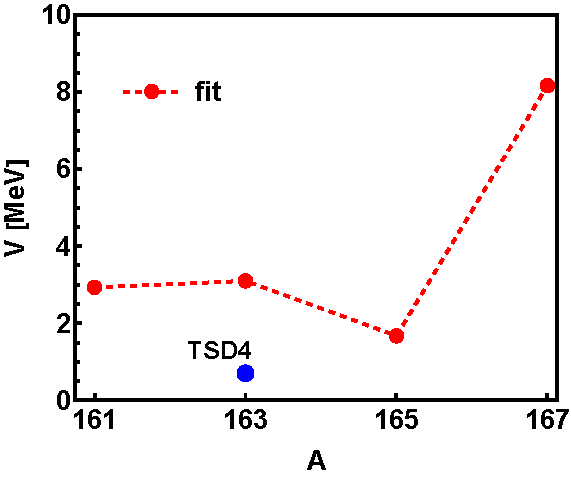
\includegraphics[scale=0.8]{Chapters/Figures/V-param-fitting.pdf}
    \caption{Fitted values for the single particle potential strength $V$ as function of the mass number $A$. The separate procedure for TSD4 in $^{163}$Lu is marked by the blue data point. The dotted line that connects each point is just to guide the eye. For an illustrative purpose, the average value across the entire mass region is also represented by the dashed horizontal line. The actual numerical values of $V$ are specified in Table \ref{numerical-fitting-parameters-Lu-isotopes}.}
    \label{fig-V-param-fitting-procedure}
\end{figure}

\subsection{Energies}

As discussed, the fitting procedure consists of a minimization for the $\chi^2$-function given in Eq. \ref{chi-2-fitting-function}, from which the `best' parameter set $\mathcal{P}_\text{fit}$ will be obtained. Having this set makes the  calculation of the theoretical values from Eq. \ref{general-excitation-energy-fitting-model} straightforward. In Fig. \ref{excitation-energies-th-161Lu}, the excitation energies of $^{161}$Lu are directly compared with the available experimental data.
\begin{figure}
    \centering
    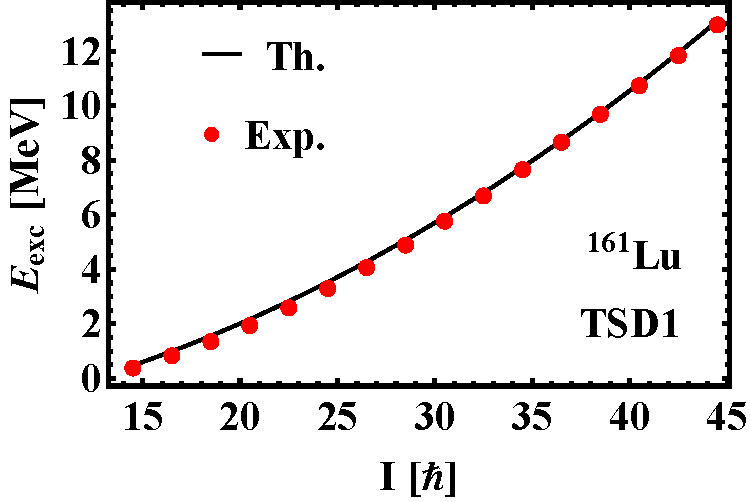
\includegraphics[width=0.49\textwidth]{Chapters/Figures/Lu-exp-energies/fig2a_lu161.pdf}
    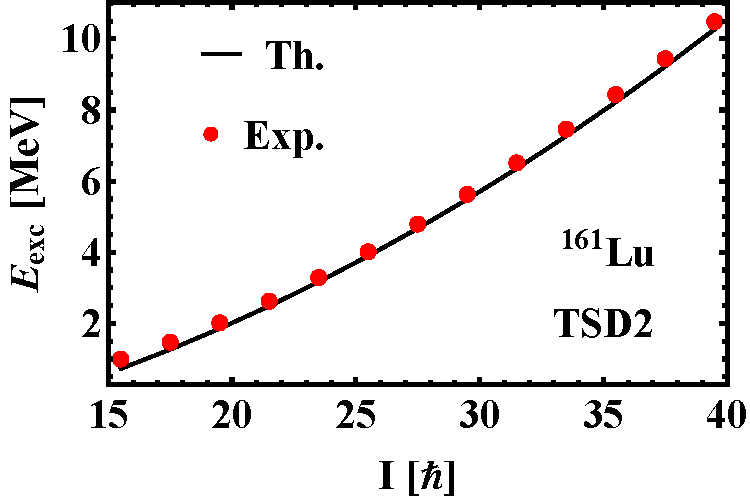
\includegraphics[width=0.49\textwidth]{Chapters/Figures/Lu-exp-energies/fig2b_lu161.pdf}
    \caption{The experimental and theoretical excitation energies provided by Eq. \ref{general-excitation-energy-fitting-model} for the two wobbling bands in $^{161}$Lu. Experimental data are taken from Ref \cite{bringel2005evidence}.}
    \label{excitation-energies-th-161Lu}
\end{figure}

The four triaxial bands of wobbling nature in $^{163}$Lu are plotted in Fig. \ref{excitation-energies-th-163Lu}, where an agreement with the experimental data can be seen across the entire spin range. When comparing the results from here with the ones of $\mathbf{W_0}$ \cite{raduta2017semiclassical}, there is a clear improvement of the present semi-classical model.
\begin{figure}
    \centering
    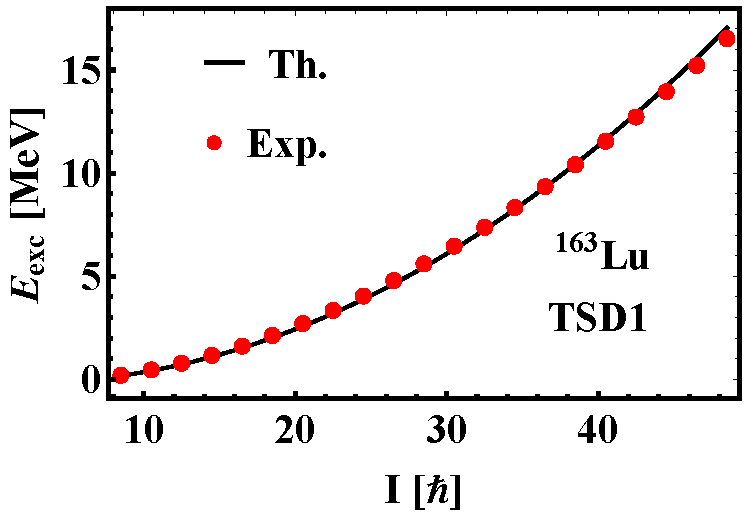
\includegraphics[width=0.49\textwidth]{Chapters/Figures/Lu-exp-energies/fig3a_lu163.pdf}
    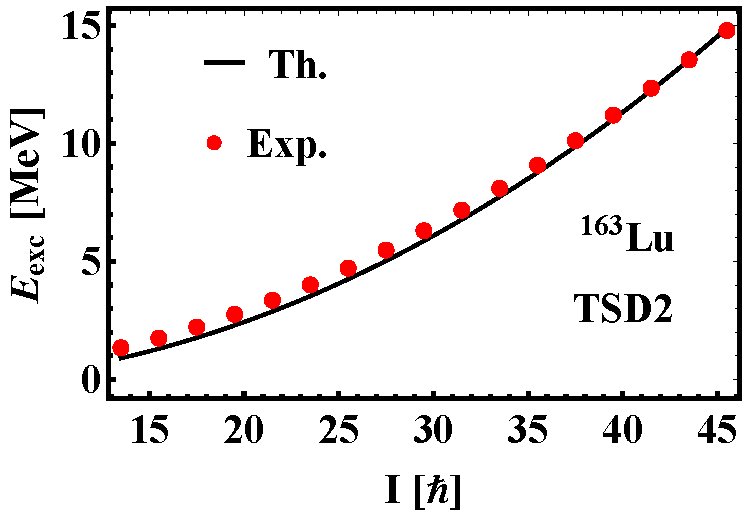
\includegraphics[width=0.49\textwidth]{Chapters/Figures/Lu-exp-energies/fig3b_lu163.pdf}
    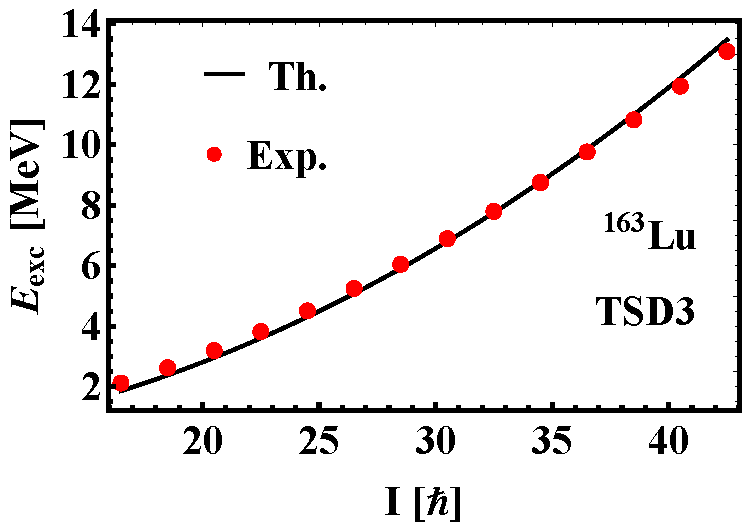
\includegraphics[width=0.49\textwidth]{Chapters/Figures/Lu-exp-energies/fig3c_lu163.pdf}
    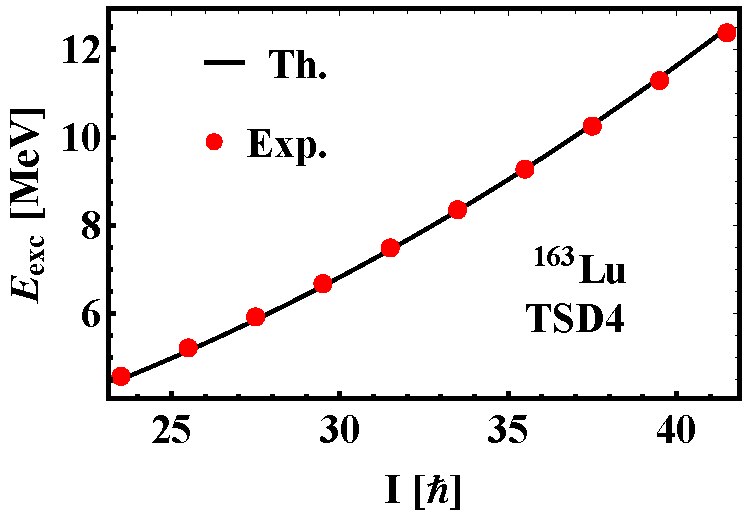
\includegraphics[width=0.49\textwidth]{Chapters/Figures/Lu-exp-energies/fig3d_lu163.pdf}
    \caption{The experimental and theoretical excitation energies provided by Eq. \ref{general-excitation-energy-fitting-model} for the two wobbling bands in $^{163}$Lu. Experimental data are taken from Ref \cite{reich2010nuclear}.}
    \label{excitation-energies-th-163Lu}
\end{figure}

A graphical representation showing the wobbling bands of $^{165}$Lu is depicted in Fig. \ref{excitation-energies-th-165Lu} as function of the total spin. From the comparison it can be seen that the two ground-bands and the one-wobbling-phonon band are fairly well reproduced through the current model.
\begin{figure}
    \centering
    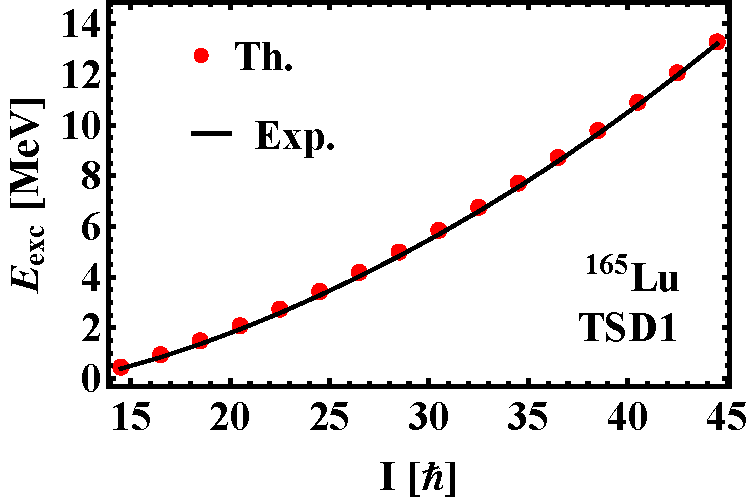
\includegraphics[width=0.32\textwidth]{Chapters/Figures/Lu-exp-energies/fig4a_lu165.pdf}
    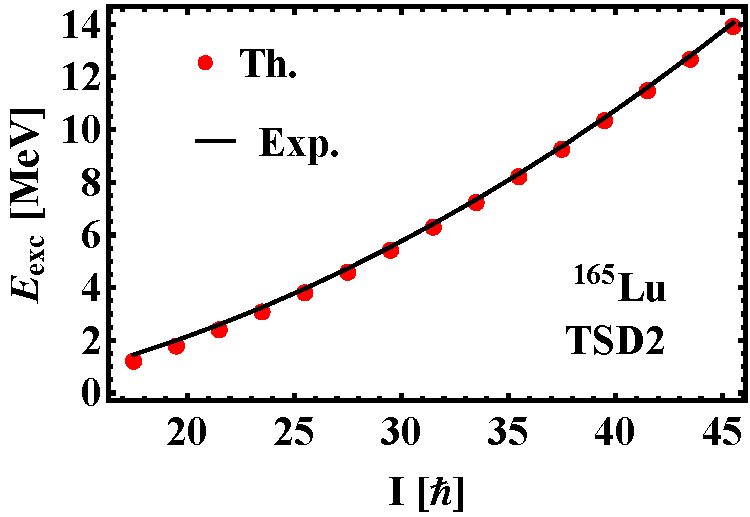
\includegraphics[width=0.32\textwidth]{Chapters/Figures/Lu-exp-energies/fig4b_lu165.pdf}
    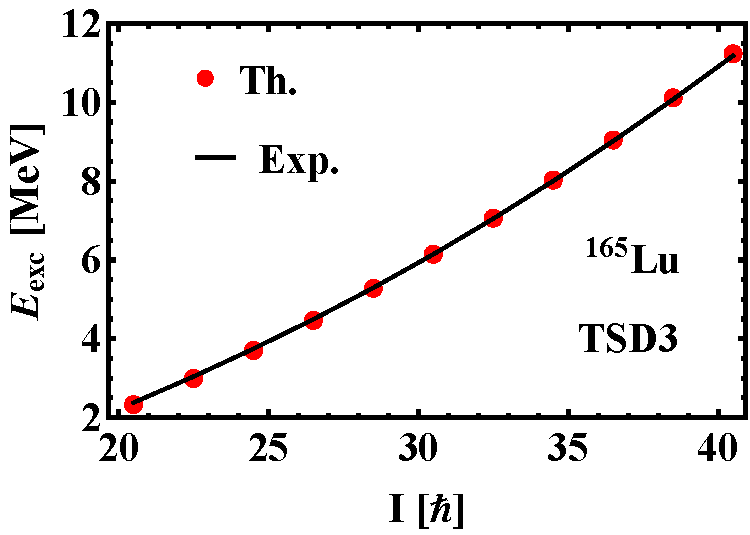
\includegraphics[width=0.32\textwidth]{Chapters/Figures/Lu-exp-energies/fig4c_lu165.pdf}
    \caption{The experimental and theoretical excitation energies provided by Eq. \ref{general-excitation-energy-fitting-model} for the three wobbling bands in $^{165}$Lu. Experimental data are taken from Ref \cite{schonwasser2003one}.}
    \label{excitation-energies-th-165Lu}
\end{figure}

Lastly, the two wobbling bands for $^{167}$Lu are shown in Fig. \ref{excitation-energies-th-167Lu} for which the experimental data are qualitatively well described by the $\mathbf{W_1}$ formalism. Based on the results summarized in Figs. \ref{excitation-energies-th-161Lu} - \ref{excitation-energies-th-167Lu}, it can be concluded that the renormalization of the wobbling structure in odd-mass nuclei was indeed a good approximation.
\begin{figure}
    \centering
    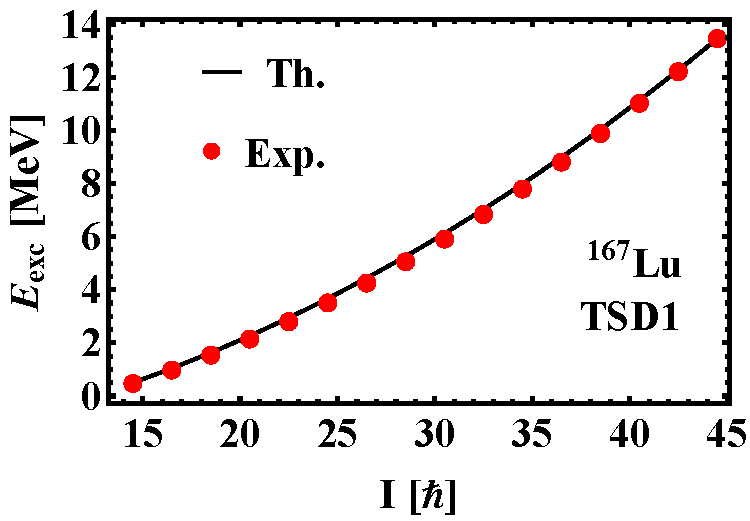
\includegraphics[width=0.49\textwidth]{Chapters/Figures/Lu-exp-energies/fig5a_lu167.pdf}
    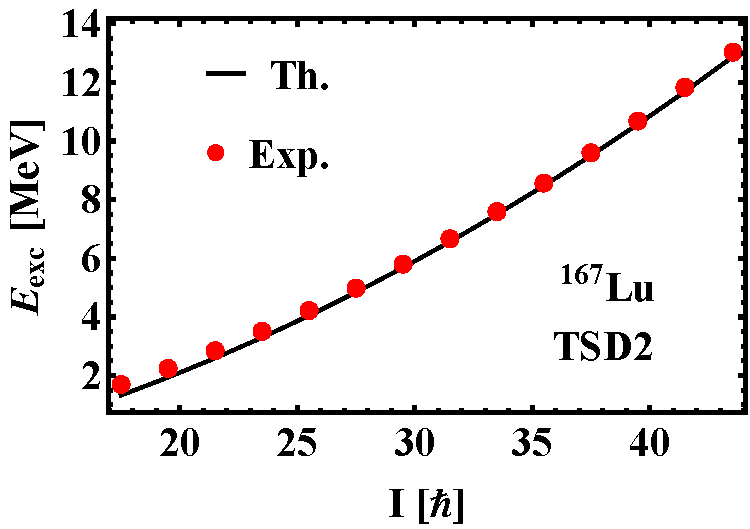
\includegraphics[width=0.49\textwidth]{Chapters/Figures/Lu-exp-energies/fig5b_lu167.pdf}
    \caption{The experimental and theoretical excitation energies provided by Eq. \ref{general-excitation-energy-fitting-model} for the three wobbling bands in $^{167}$Lu. Experimental data are taken from Ref \cite{amro2003wobbling}.}
    \label{excitation-energies-th-167Lu}
\end{figure}

In what follows a remark about the evidence towards a transverse/longitudinal wobbling regime should be made. Indeed, if one recalls the behavior of the wobbling energy defined in the sense of Eq. \ref{eq-wobbling-energy-definition-oddA} for the $A\approx160$ region, all isotopes show a decreasing trend with respect to the total angular momentum. Such a decrease would indicate the transverse-like regime for every isotope. However, the evaluation of $E_\text{wob}$ from Eq. \ref{eq-wobbling-energy-definition-oddA} implies that the $n_w=1$ band is always the first band above the yrast line. By contrast, in this approach, the $n_w=1$ band only appears for $^{163,165}$Lu nuclides due to them having states activated by the phonon operator $\Gamma^\dagger$ from TSD2. Consequently, a direct comparison between the experimental and theoretical values can be made solely for the set of states $\text{TSD3}\to\text{TSD2}$, meaning that the standard definition for the wobbling energy is now properly adjusted to the $\mathbf{W_1}$ formalism and the graphical representation is done in Fig. \ref{experimental-wobbling-energies-Lu-aw1}. Based on the plots, it can be seen that the experimental wobbling energy is increasing from $0.144$ MeV to $0.170$ MeV within the spin range $[33/2,77/2]$ and then it decreases for the last two spin states. Interesting the fact that both isotopes have a rather similar behavior for the experimental $E_\text{wob}$, although at the high-spin limit the decrease in magnitude is unexpected because the core and the quasi-particle's a.m. must point in the same direction, thus leading to longitudinal-like motion. Additionally, the current theory predicts the increasing part and it even shows a slight quenching when $I\geq 40\hbar$. Besides that, there is an almost constant shift between the calculated and experimental values for $E_\text{wob}$ of about $\approx 0.3\ \text{MeV}$ and $\approx 0.15\ \text{MeV}$ in $^{163}$Lu and $^{165}$Lu, respectively. One may conclude that the present model properly describes the wobbling motion, which is also consistent with microscopic studies done in Ref. \cite{matsuzaki2002wobbling}.
\begin{figure}
    \centering
    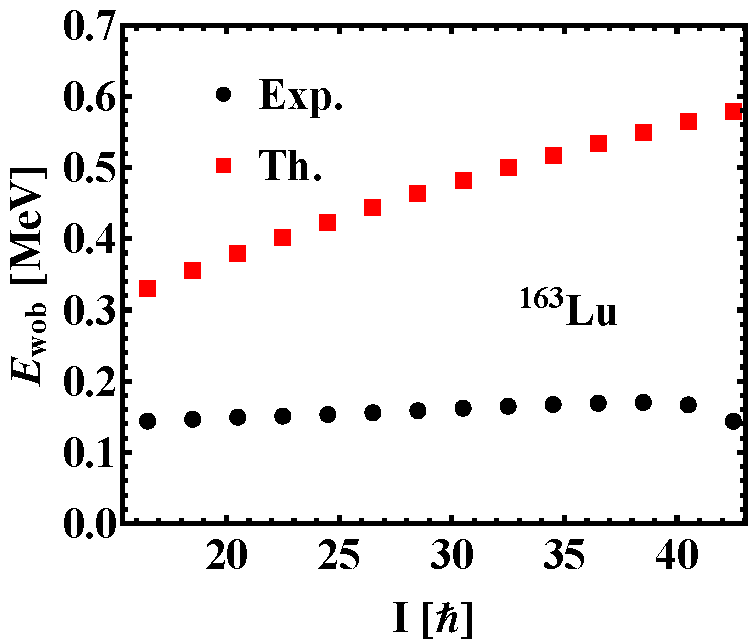
\includegraphics[width=0.49\textwidth]{Chapters/Figures/Lu-exp-energies/fig6a.pdf}
    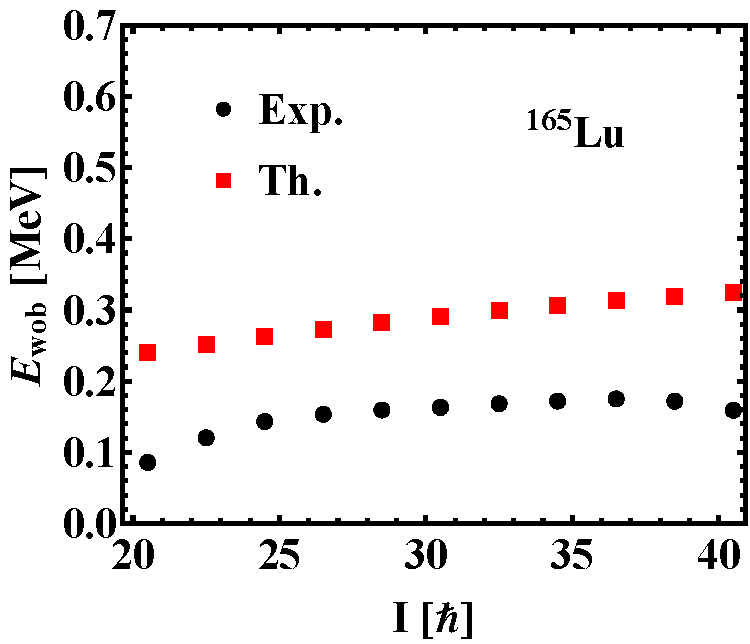
\includegraphics[width=0.49\textwidth]{Chapters/Figures/Lu-exp-energies/fig6b.pdf}
    \caption{The theoretical wobbling energies as per Eq. \ref{eq-wobbling-energy-definition-oddA} compared with the experimental ones, for the isotopes $^{163}$Lu (\textbf{left}) and $^{165}$Lu (\textbf{right}). Note that the $n=1$ and $n=0$ bands are TSD3 and TSD2 within the current description.}
    \label{experimental-wobbling-energies-Lu-aw1}
\end{figure}

\subsection{Alignment}

Going further with the study of the triaxial properties in odd-mass nuclei, other relevant quantities are calculated within the current formalism. The \emph{alignment} (or aligned angular momentum) is defined as the total spin minus a reference value. Usually the reference value is a function that is cubed in the rotational frequency $\hbar\omega$. Namely the alignment and its reference value are given as:
\begin{align}
    i_x=&I-I_\text{ref}\ ,\nonumber\\
    I_\text{ref}=&\mathcal{I}_0\omega+\mathcal{I}_1\omega^3\ ,
    \label{alignment-reference-angular-momentum}
\end{align}
where the coefficients $\mathcal{I}_0$ and $\mathcal{I}_1$ are obtained by a least square procedure fit. Within literature, these values are also known as the Harris parameters \cite{harris1965higher}. The linear term from Eq. \ref{alignment-reference-angular-momentum} is involved in the spherical symmetry and the second term is related to the axial symmetry. Consequently, the alignment gives a measure of triaxiality for the isotopes. The comparison between the theoretical and the experimental alignments is done for each isotope with the Harris parameters set to $\left(\mathcal{I}_0,\mathcal{I}_1\right)=\left(30,40\right)$ in units of $\hbar^2\text{MeV}^{-1}$, and the results can be seen in Fig. \ref{alignments-lu-163} for $^{163}$Lu, Fig. \ref{alignments-lu-165} for $^{165}$Lu, and lastly Fig. \ref{alignments-lu-161-167} for $^{161}$Lu and $^{167}$Lu.
\begin{figure}
    \centering
    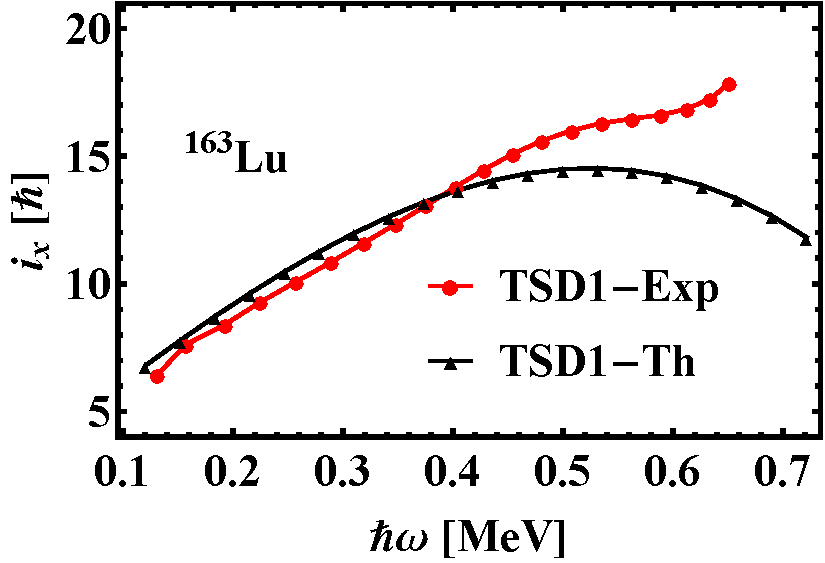
\includegraphics[width=0.49\textwidth]{Chapters/Figures/Lu-exp-energies/fig8a_lu163.pdf}
    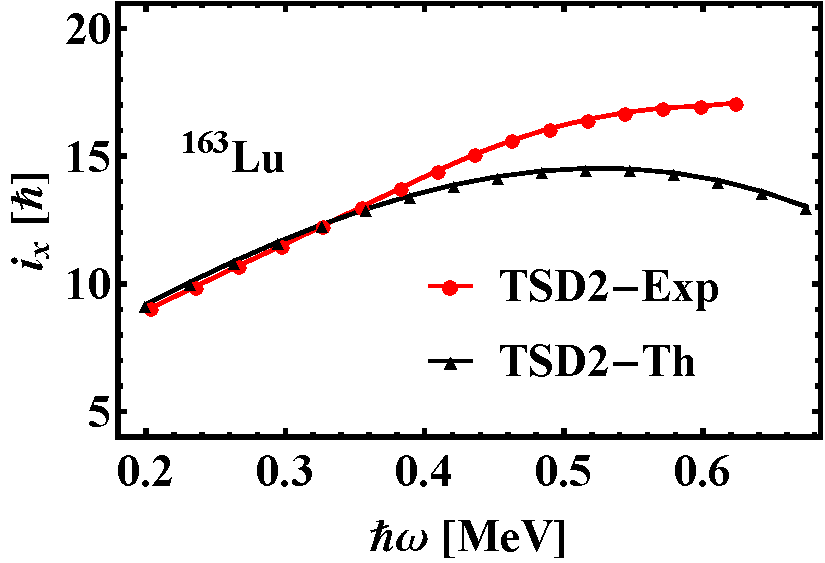
\includegraphics[width=0.49\textwidth]{Chapters/Figures/Lu-exp-energies/fig8b_lu163.pdf}
    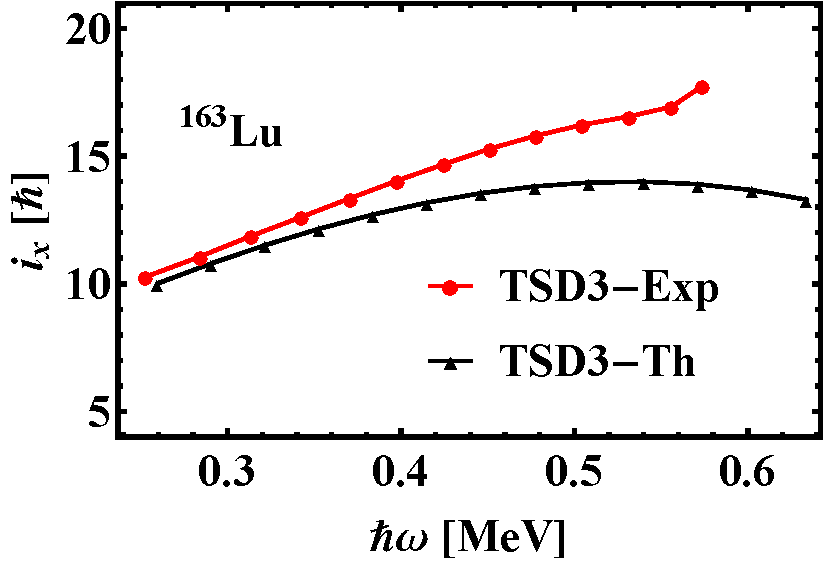
\includegraphics[width=0.49\textwidth]{Chapters/Figures/Lu-exp-energies/fig8c_lu163.pdf}
    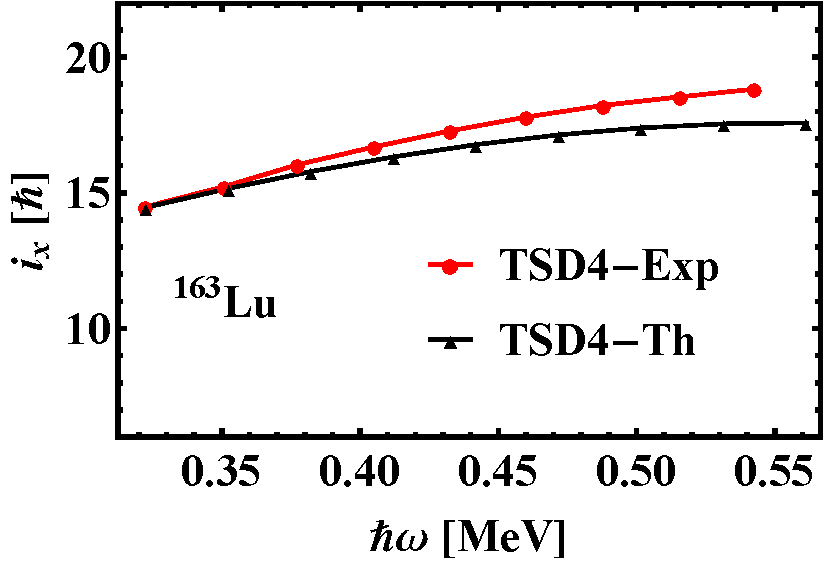
\includegraphics[width=0.49\textwidth]{Chapters/Figures/Lu-exp-energies/fig8d_lu163.pdf}
    \caption{The theoretical and experimental alignments for $^{163}$Lu, according to Eq. \ref{alignment-reference-angular-momentum}, as function of the rotational frequency (Eqs. \ref{rotational-frequency-canonical-definition} - \ref{rotational-frequency-canonical}). Even though TSD4 was fitted separately for calculations of Eq. \ref{general-excitation-energy-fitting-model}, the same Harris parameters were employed as in TSD1-2-3.}
    \label{alignments-lu-163}
\end{figure}
\begin{figure}
    \centering
    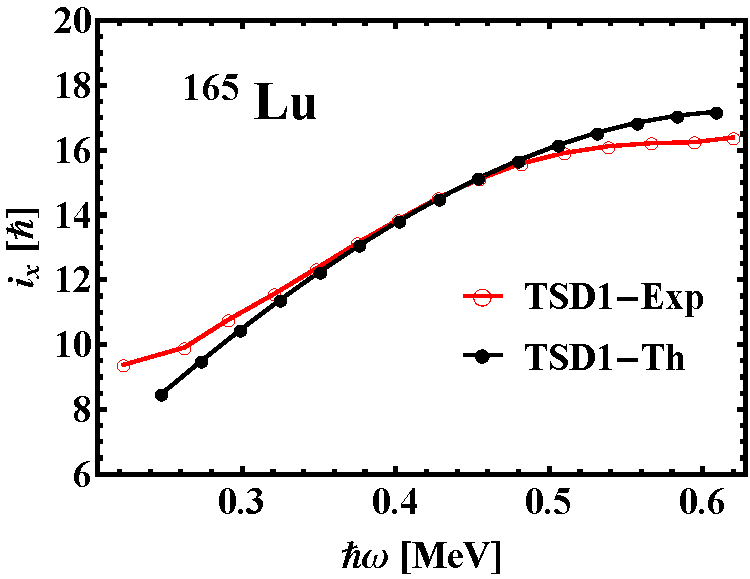
\includegraphics[width=0.49\textwidth]{Chapters/Figures/Lu-exp-energies/fig9a_lu165.pdf}
    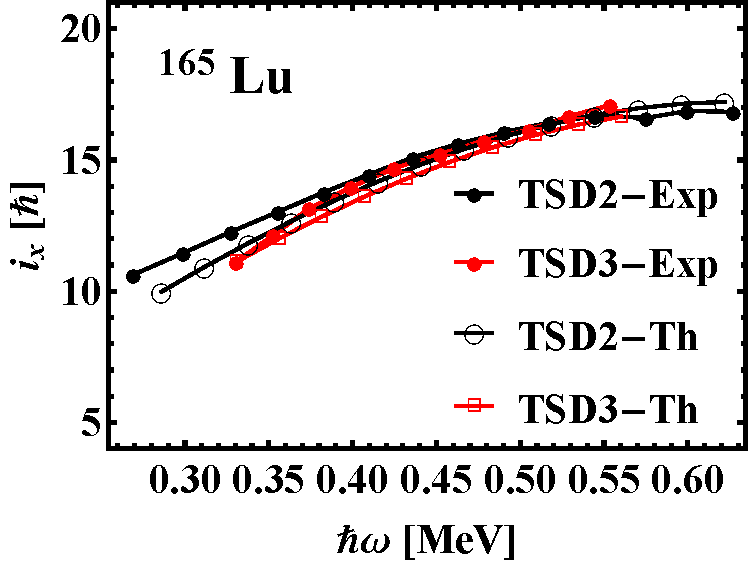
\includegraphics[width=0.49\textwidth]{Chapters/Figures/Lu-exp-energies/fig9b_lu165.pdf}
    \caption{The theoretical and experimental alignments for $^{165}$Lu, according to Eq. \ref{alignment-reference-angular-momentum}, as function of the rotational frequency (Eqs. \ref{rotational-frequency-canonical-definition} - \ref{rotational-frequency-canonical}). The numerical evaluation was done with the Harris parameters defined in text.}
    \label{alignments-lu-165}
\end{figure}
\begin{figure}
    \centering
    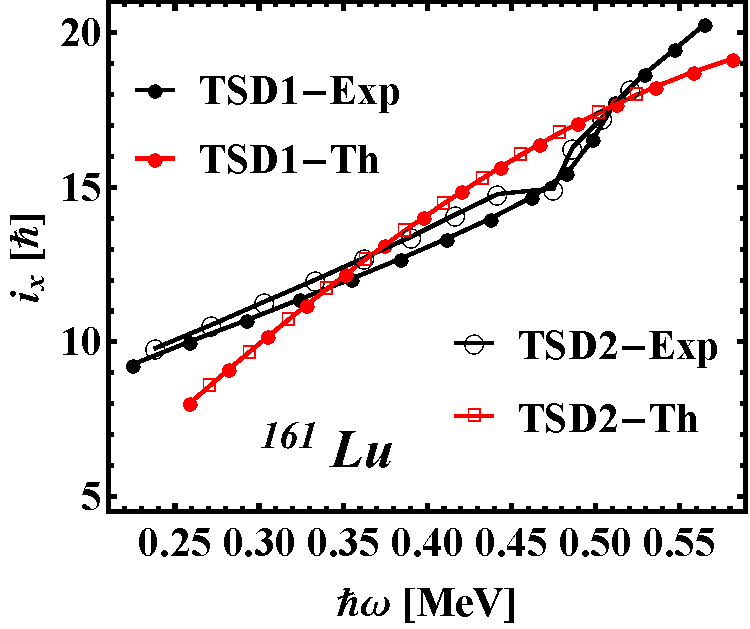
\includegraphics[width=0.49\textwidth]{Chapters/Figures/Lu-exp-energies/fig7.pdf}
    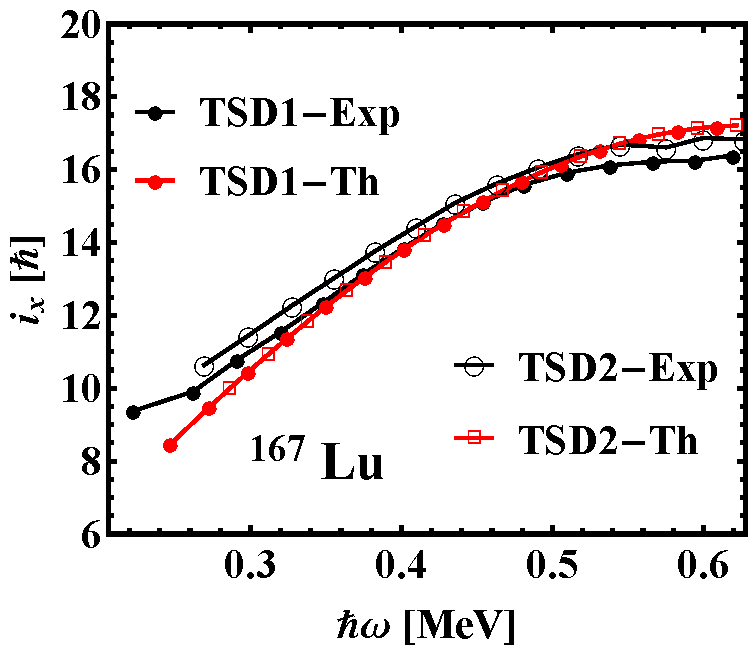
\includegraphics[width=0.49\textwidth]{Chapters/Figures/Lu-exp-energies/fig10.pdf}
    \caption{The theoretical and experimental alignments for $^{161}$Lu (\textbf{left}) and $^{167}$Lu (\textbf{right}), according to Eq. \ref{alignment-reference-angular-momentum}, as function of the rotational frequency (Eqs. \ref{rotational-frequency-canonical-definition} - \ref{rotational-frequency-canonical}). The numerical evaluation was done with the Harris parameters defined in text.}
    \label{alignments-lu-161-167}
\end{figure}

Taking a closer look at Figs. \ref{alignments-lu-163} - \ref{alignments-lu-161-167}, a good agreement between the theory and experiment can be inferred, especially for $A=167$. There are however a few discrepancies between the results for $^{163}$Lu in the high-frequency limit (i.e., $\hbar\omega\geq 0.45\ \text{MeV}$), where the experimental data shows a rather linear increase while the theoretical points seem to suffer a quenching with a slight down-bending. In fact, one might extract three regions each with its different character regarding the angular momentum: a) one linearly increasing region at small frequencies ($\hbar\omega\in[0,0.3]$), b) a saturation region at medium frequencies ($\hbar\omega\in[0.3,0.55]$), and finally c) a decreasing function at high frequencies ($\hbar\omega\geq 0.6$). It seems that $\mathbf{W_1}$ can be further improved if the alignment is properly adjusted (e.g., by amending it with a linear term having large contribution only in the upper $\hbar\omega$-limit).

Comparing the curves relative to the entire mass region, based on their similarities and the fact that they are quite close to each other indeed reflects the wobbling character. Using $\mathbf{W_0}$, some alignment values were evaluated for $^{165}$Lu and $^{167}$Lu \cite{raduta2018wobbling}, where the bands TSD2 and TSD3 were one- and two-wobbling phonons. This new approach theory shows a clear improvement over the previous model.

\subsection{Reference Energy}

Another useful quantity that could illustrate a wobbling behavior across neighboring isotopes is the excitation energy relative to a spherical rigid rotor. This is evaluated with an \emph{effective} moment of inertia and it is graphically represented as function of the total angular momentum. In principle, the reference energy is a typical rotor expression defined in terms of the squared angular momentum as $E_\text{ref}=\alpha I(I+1)$. The value of $\alpha$ can be indeed regarded as an effective inverse MOI, which is usually determined by fitting the experimental reference energies. Moreover, $\alpha$ can differ from isotope to isotope but here one kept the same value across all nuclides (for consistency), and the obtained numerical results show a fairly good agreement with the experimental data set.

Throughout the current calculations, the reference energy was fixed to $E_\text{ref}=0.0075I(I+1)\ \text{MeV}$. The results are depicted in Fig. \ref{reference-rotor-energy-lu161} for $^{161}$Lu, Fig. \ref{reference-rotor-energy-lu165} for $^{165}$Lu, and Fig. \ref{reference-rotor-energy-lu167} for $^{167}$Lu. The four wobbling bands in $^{163}$Lu are each plotted separately in Fig. \ref{reference-rotor-energy-lu163}.
\begin{figure}
    \centering
    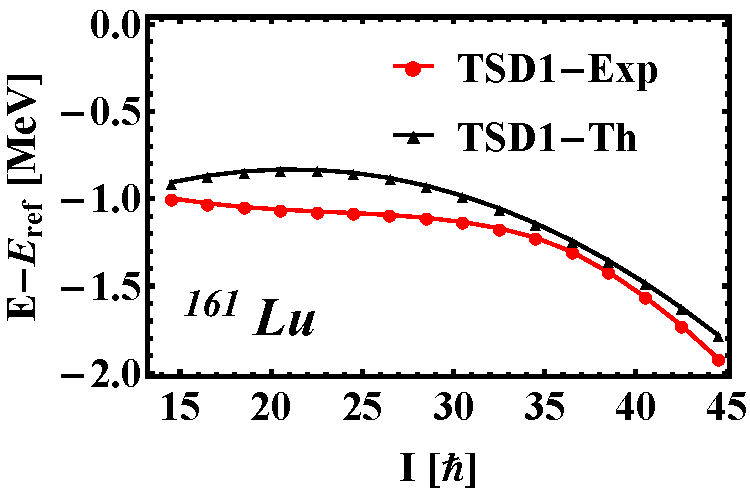
\includegraphics[width=0.49\textwidth]{Chapters/Figures/Lu-exp-energies/fig11a_lu161.pdf}
    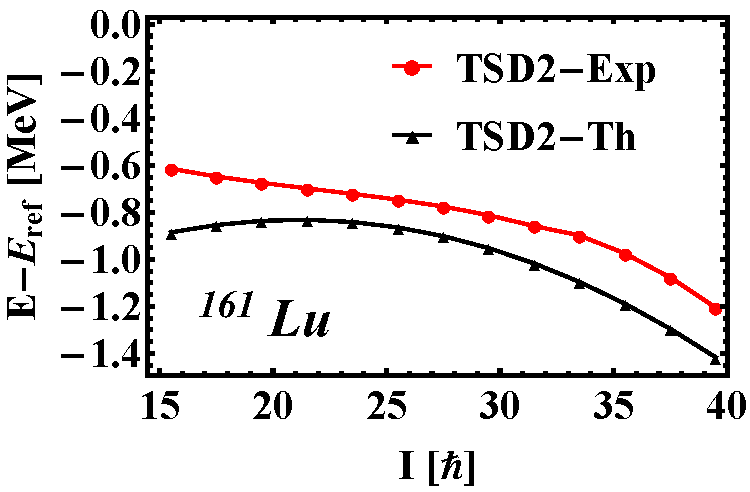
\includegraphics[width=0.49\textwidth]{Chapters/Figures/Lu-exp-energies/fig11b_lu161.pdf}
    \caption{The excitation energy relative to a rotor reference $E_\text{ref}=0.0075I(I+1)$ as function of the total angular momentum, for $^{161}$Lu.}
    \label{reference-rotor-energy-lu161}
\end{figure}
\begin{figure}
    \centering
    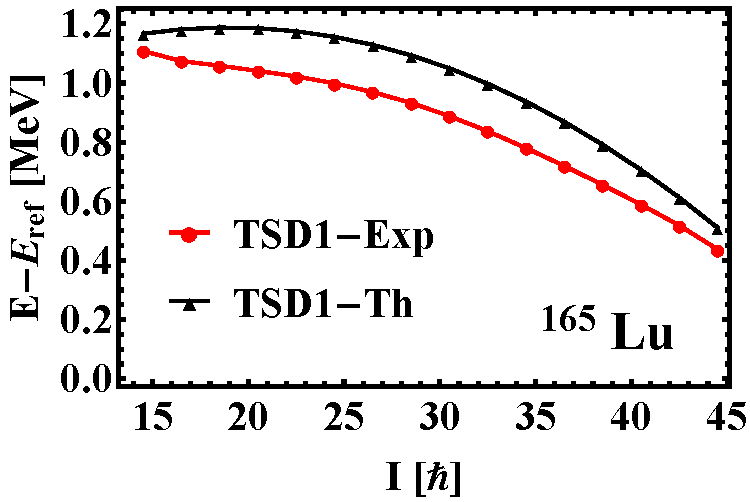
\includegraphics[width=0.49\textwidth]{Chapters/Figures/Lu-exp-energies/fig13a_lu165.pdf}
    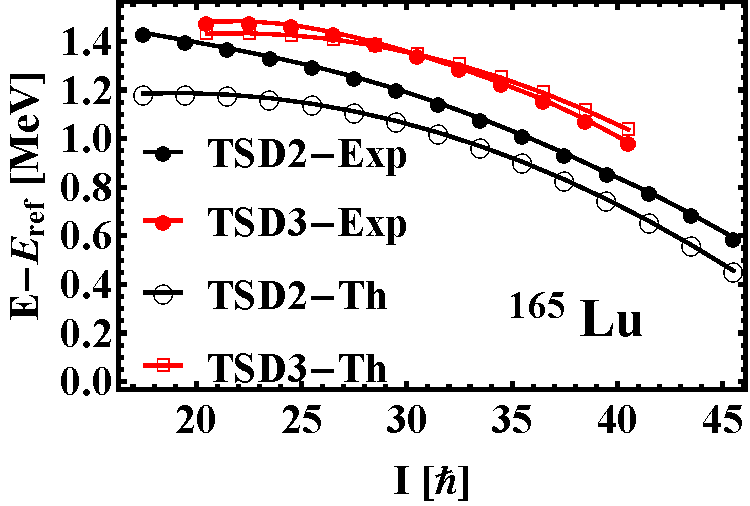
\includegraphics[width=0.49\textwidth]{Chapters/Figures/Lu-exp-energies/fig13b_lu165.pdf}
    \caption{Comparison between theoretical and experimental excitation energy relative to a rotor reference $E_\text{ref}=0.0075I(I+1)$ for $^{165}$Lu, as function of the total angular momentum. The zero- and one-wobbling-phonon bands TSD2-3 are plotted on the same figure.}
    \label{reference-rotor-energy-lu165}
\end{figure}
\begin{figure}
    \centering
    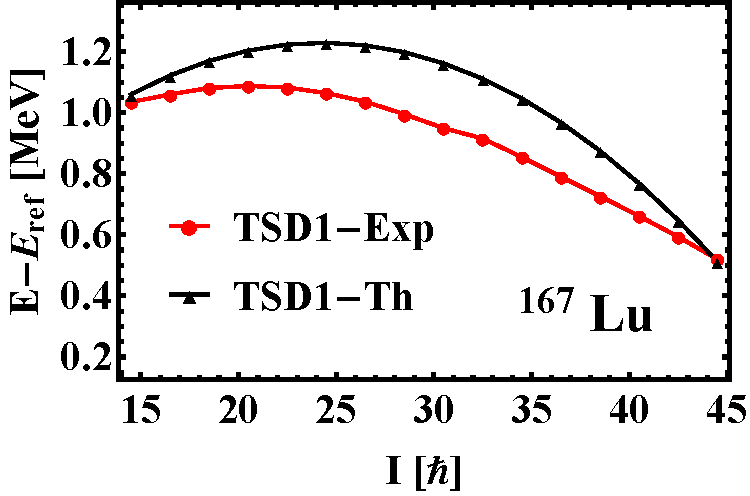
\includegraphics[width=0.49\textwidth]{Chapters/Figures/Lu-exp-energies/fig14a_lu167.pdf}
    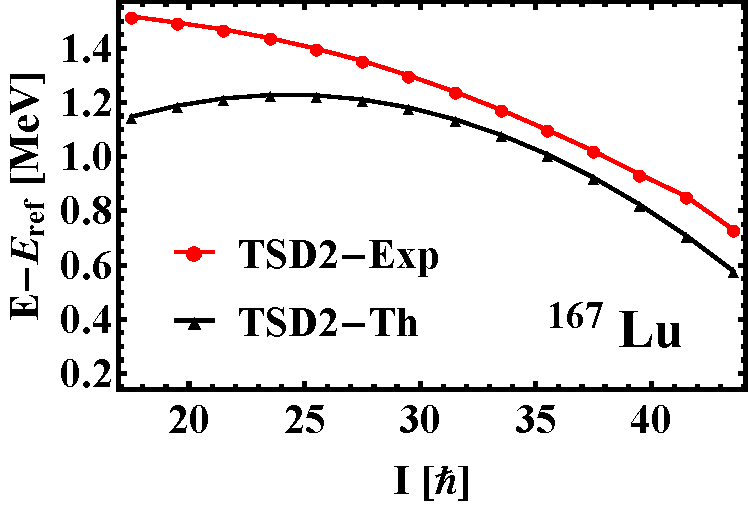
\includegraphics[width=0.49\textwidth]{Chapters/Figures/Lu-exp-energies/fig14b_lu167.pdf}
    \caption{Comparison between theoretical and experimental excitation energy relative to a rotor reference $E_\text{ref}=0.0075I(I+1)$ for $^{167}$Lu, as function of the total angular momentum.}
    \label{reference-rotor-energy-lu167}
\end{figure}
\begin{figure}
    \centering
    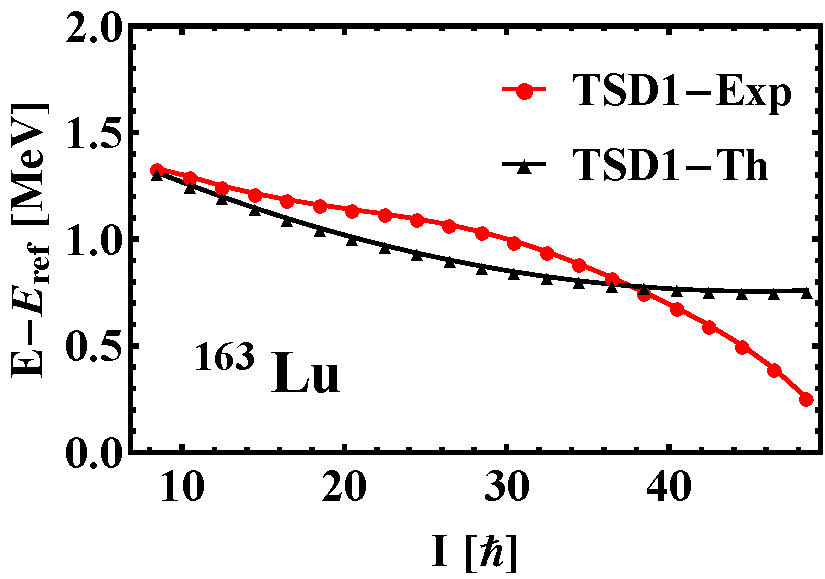
\includegraphics[width=0.49\textwidth]{Chapters/Figures/Lu-exp-energies/fig12a_lu163.pdf}
    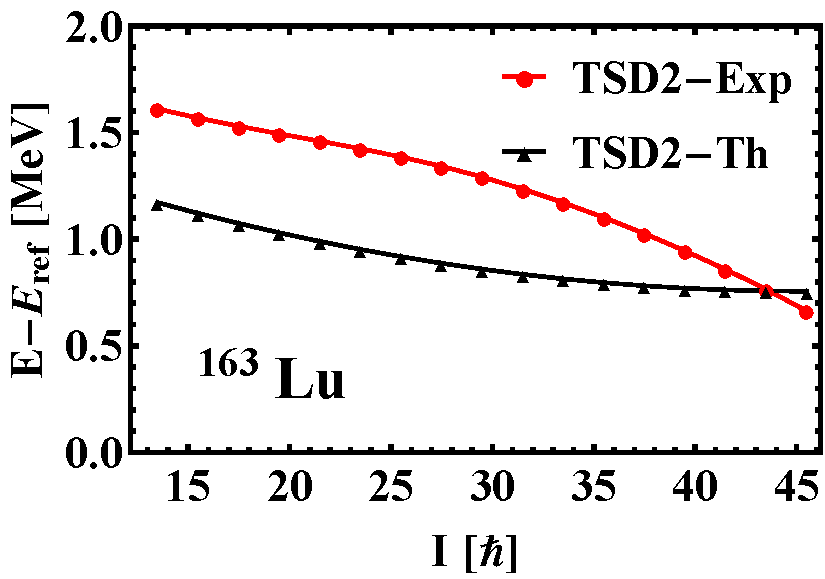
\includegraphics[width=0.49\textwidth]{Chapters/Figures/Lu-exp-energies/fig12b_lu163.pdf}
    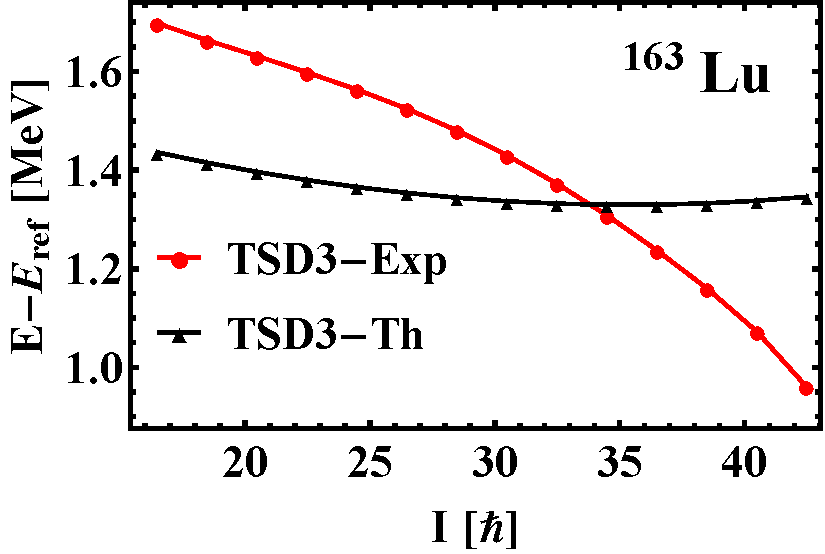
\includegraphics[width=0.49\textwidth]{Chapters/Figures/Lu-exp-energies/fig12c_lu163.pdf}
    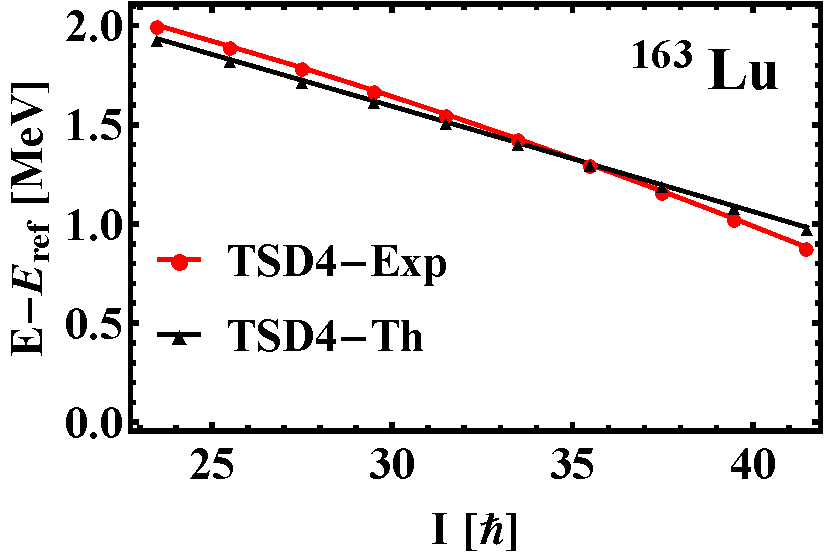
\includegraphics[width=0.49\textwidth]{Chapters/Figures/Lu-exp-energies/fig12d_lu163.pdf}
    \caption{The excitation energy relative to a rotor reference $E_\text{ref}=0.0075I(I+1)$ as function of the total angular momentum, for $^{163}$Lu.}
    \label{reference-rotor-energy-lu163}
\end{figure}

Concerning the graphical representations from Figs. \ref{reference-rotor-energy-lu161} - \ref{reference-rotor-energy-lu163}, some remarks should be highlighted. Firstly, each experimental curve shows a decreasing trend with angular momentum. Some bands exhibit a stronger behavior than others. For example, TSD2 of $^{163}$Lu is almost constant in the range $I\in[15-17]\ \hbar$ and only starts to get smaller beyond when $I\geq 30\hbar$. The same can be observed for TSD3 from $^{165}$Lu. On the other hand, TSD3 from $^{163}$Lu or TSD2 from $^{167}$Lu are decreasing rather rapidly across the entire spin range. The reduction of $E-E_\text{ref}$ indicates that the contribution of the rotor part becomes more and more significant, leading to a diminishing effect of triaxiality when angular momentum reaches large values. The theoretical curves do reproduce the overall trends, showing some striking similarities for TSD4 from $^{163}$Lu or TSD3 in $^{165}$Lu. Remarking that the obtained numerical data for TSD1-2-3 from $^{163}$Lu show a decrease within a \emph{convex} manner, whereas the experimental sets behave as \emph{concave} functions. The deviation from the experimental set for TSD3 in the same nucleus increases by about 0.3 MeV for $I\geq 35\hbar$. Otherwise, it can be concluded that the current model does reproduce the dominance of a rotor-like behavior over triaxiality at large angular momentum for the studied isotopes. Improvements in the quality of the figures can be observed when comparing with the calculations made using the previous approach $\mathbf{W_0}$ \cite{raduta2018wobbling}.

\subsection{Dynamic MOI}

The dynamic moment of inertia $\mathcal{I}^{(2)}$ was introduced in Chapter \ref{chapter-3} (recall Eqs. \ref{dynamic-moi-general} - \ref{dynamic-moi-energy-levels}), where it was shown that this quantity is directly related to the energy differences for the $I+2,I,I-2$ levels, respectively. Usually $\mathcal{I}^{(2)}$ is represented as a function of the rotational frequency or even the total angular momentum. In the current model, the graphical representations are made with respect to the rotational frequency and the data for $^{161,167}$Lu can be seen in Fig. \ref{dynamic-moi-Lu-161-167}. For $^{163}$Lu, the comparison between theory and experiment concerning $\mathcal{I}^{(2)}$ is depicted in Fig. \ref{dynamic-moi-Lu-163}. Lastly, the three bands from $^{165}$Lu are sketched in Fig. \ref{dynamic-moi-Lu-165}.
\begin{figure}
    \centering
    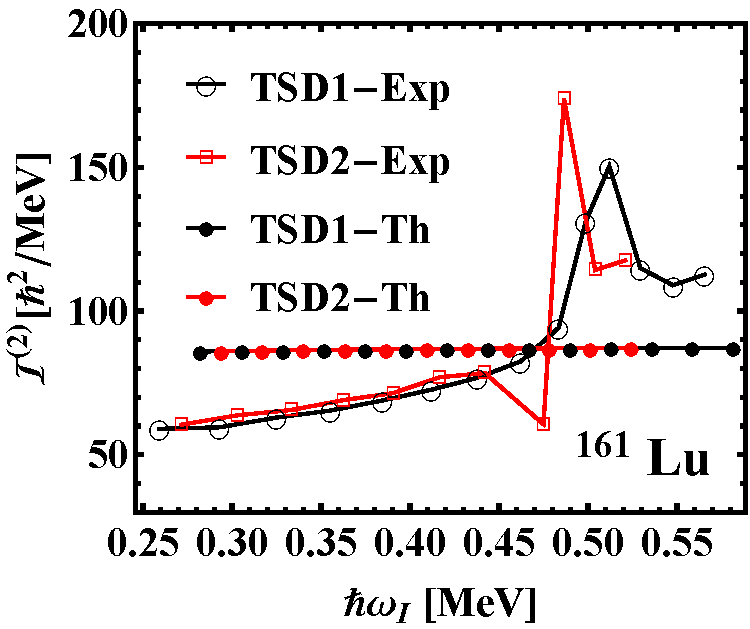
\includegraphics[width=0.49\textwidth]{Chapters/Figures/Lu-exp-energies/fig15_lu161.pdf}
    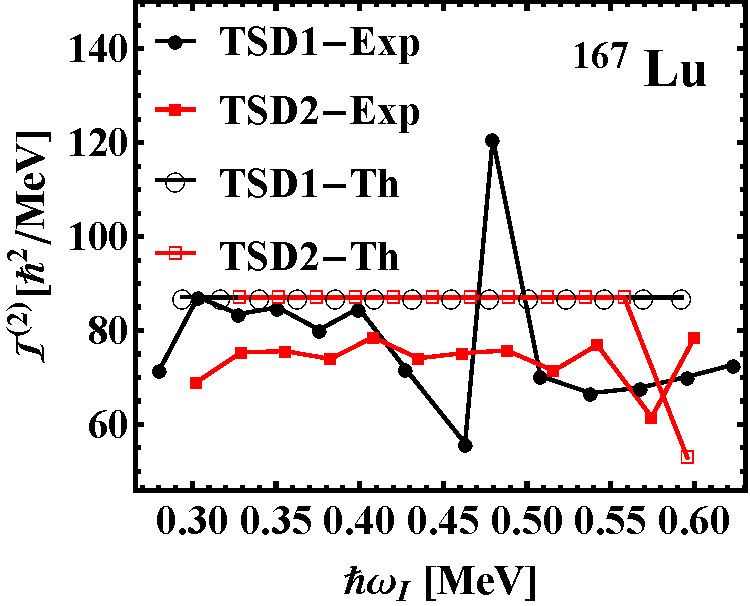
\includegraphics[width=0.49\textwidth]{Chapters/Figures/Lu-exp-energies/fig18_lu167.pdf}
    \caption{The theoretical dynamic moment of inertia defined in Eq. \ref{dynamic-moi-general} for the isotopes $^{161}$Lu (\textbf{left}) and $^{167}$Lu (\textbf{right}) is compared with the experimental data. The rotational frequency is defined as $\hbar\omega_I=\text{d}E/\text{d}I=E_\gamma(I,I-2)/2$.}
    \label{dynamic-moi-Lu-161-167}
\end{figure}
\begin{figure}
    \centering
    \includegraphics[width=0.496\textwidth]{Chapters/Figures/Lu-exp-energies/fig16a_lu163.pdf}
    \includegraphics[width=0.49\textwidth]{Chapters/Figures/Lu-exp-energies/fig16b_lu163.pdf}
    \caption{The dynamic moment of inertia defined in Eq. \ref{dynamic-moi-general} for $^{163}$Lu. The rotational frequency is defined as $\hbar\omega_I=\text{d}E/\text{d}I=E_\gamma(I,I-2)/2$.}
    \label{dynamic-moi-Lu-163}
\end{figure}
\begin{figure}
    \centering
    \includegraphics[width=0.49\textwidth]{Chapters/Figures/Lu-exp-energies/fig17a_lu165.pdf}
    \includegraphics[width=0.49\textwidth]{Chapters/Figures/Lu-exp-energies/fig17b_lu165.pdf}
    \caption{The dynamic moment of inertia defined in Eq. \ref{dynamic-moi-general} for $^{165}$Lu showing the band TSD1 (\textbf{left}) and the bands TSD2-3 (\textbf{right}). The rotational frequency is defined as $\hbar\omega_I=\text{d}E/\text{d}I=E_\gamma(I,I-2)/2$.}
    \label{dynamic-moi-Lu-165}
\end{figure}

Usually, the dynamic MOI is sensitive to the single-particle effects, such as alignment of nucleons or even interaction between states belonging to different bands. As such, it could be a useful indicator of triaxiality and wobbling motion, since the nucleus can suffer structural changes as its angular momentum (and implicitly rotational frequency) increases. Looking at the figures with $\mathcal{I}^{(2)}$ for each isotope, some interesting features appear. Firstly, regarding the theoretical calculations, $\mathbf{W_1}$ formalism predicts constant values for this quantity, meaning that the dynamic MOI is a constant function of $\hbar\omega$ and furthermore the rotational frequency is linear in $I$. This can be indeed observed throughout the plots, where each TSD band has a constant $\mathcal{I}^{(2)}$ for the entire range of $\hbar\omega$. Nonetheless, if one `averages out' the experimental set of points to a singular value for each band, the theoretical and experimental lines would lie quite close to each other. On the other side, for the experimental data there is a staggering present (e.g., band TSD1 from $^{161}$Lu) and even sharp changes in magnitude, as it is the case for TSD2 from $^{161}$Lu and $^{165}$Lu, respectively. In $^{161}$Lu, for example, the abrupt increase is caused by the alignment of the odd-proton's a.m., showing up at $\hbar\omega=0.45\ \text{MeV}$. The staggering behavior in the triaxial bands of the isotopes, mostly appearing in the low $\hbar\omega$ region, is caused by interaction between the states from the TSD bands and their neighboring normally deformed structures. Remarkable the fact that TSD1 from $^{165}$Lu exhibits a rather constant dynamic MOI (just as the  theoretical value) except for the first two states. Comparing the present calculations with the results from Ref. \cite{raduta2018wobbling}, an overall improvement in the agreement with the experimental data can be observed.

\subsection{Electromagnetic Transitions}

In this section, the electromagnetic transitions for $^{161,163,165,167}$Lu will be calculated within the $\mathbf{W_1}$ formalism and compared with the available experimental data. For collective phenomena, one usually expects two `main' characteristics to arise: a) the transitions between neighboring bands to be predominantly of E2 character and b) the states have large quadrupole moments. In fact, as it was discussed in Chapters \ref{chapter4} and \ref{chapter-5}, the large quadrupole moments and large mixing ratios $\delta$ are regarded as essential `tests' for wobbling behavior.

For the numerical application, in the first part the electric quadrupole E2 transitions will be discussed, while in the second part the magnetic dipole M1 transitions are addressed. Concerning the states, the transitions between two states inside the same band (=intraband) as well as the transitions between adjacent bands (=interband) need to be evaluated. Because of the collective nature of the wobbling bands, the spin difference within a band is $\Delta I=2$ units of angular momentum, while two states from adjacent bands only differ by one unit $\Delta I=1$ (recall Fig. \ref{wobbling-geometry-tilting-sketch} from the discussion in Chapter \ref{chapter-5}). A schematic representation that illustrates the difference between interband/intraband transitions can be seen in Fig. \ref{schematic-interband-intraband-E2}. Therein, the E2 transitions are sketched for levels belonging to the same band and levels from different bands, and for each band the allowed spin sequences are exemplified. The magnetic transitions for wobbling states have a dipole nature, which means that they take place between states that differentiate by one unit of angular momentum. Experimental observations point out that in collective spectra these M1 transitions are typically quite small in comparison with the E2 ones. Moreover, the `competition' between E2 and M1 for a state $I$ is reflected in the mixing ratio $\delta$, which is expected to be large for the studied isotopes. 
\begin{figure}
    \centering
    \includegraphics[scale=1.1]{Chapters/Figures/transitions-wobbling-states.pdf}
    \caption{Schematic representation with the electric quadrupole transitions occurring in wobbling spectra of nuclei. The \emph{intraband} values ($E2_\text{in}$ ; blue) represent the transitions between an initial state $I_\text{i}$ and an final state $I_\text{f}$ belonging to the same band, which are characterized by $\Delta I=I_\text{i}-I_\text{f}=2\hbar$. On the other hand, the \emph{interband} values ($E2_\text{out}$ ; red) take place between states belonging to two contiguous bands, and they are characterized by $\Delta I=1\hbar$. The spin sequences for each band are given below the level schemes in curly brackets.}
    \label{schematic-interband-intraband-E2}
\end{figure}

The transition probabilities between states that comprise the excited spectra can be determined from the matrix elements (m.e.) of the \emph{electromagnetic transition operators} (recall discussion in Section \ref{intro-EM-chapter3} from Chapter \ref{chapter-3}). The calculations are made in the laboratory (lab) system, meaning that the multipole operators must be expressed in terms of the \emph{intrinsic} ones via the Wigner-$\mathcal{D}$ functions \cite{toki1975asymmetric,bohr1998nuclear}:
\begin{align}
    \mathcal{M}(\lambda,\mu)=\sum_\nu\mathcal{D}_{\mu\nu}^\lambda\mathcal{M}(\lambda,\nu)\ ,
    \label{multipole-operator-lab}
\end{align}
where $\mathcal{M}(\lambda,\mu)$ represents the lab operator and $\mathcal{M}(\lambda,\nu)$ is the intrinsic multipole operator. The quantities of interest here are $\mathcal{M}(E2,\mu)$ for the electric quadrupole transitions and $\mathcal{M}(M1,\mu)$ for the magnetic dipole transitions. Each case will be treated individually in the following subsections, starting with the analytical expressions and finally providing the numerical results.

\subsubsection{E2 Transitions}

For the E2 transitions, one has to replace $\lambda=2$ in Eq. \ref{multipole-operator-lab}, and the \emph{quadrupole transition operator} becomes \cite{toki1975asymmetric,raduta2020towards}:
\begin{align}
    \mathcal{M}(E2,\mu)=\left[\mathcal{D}_{\mu0}^2Q_0-\left(D_{\mu 2}^2+D_{\mu -2}^2\right)Q_2\right]+\mathrm{e}\sum_{\nu=-2,0,2}\mathcal{D}_{\mu\nu}^2r^2Y_2^\nu\ .
    \label{electric-quadrupole-operator-lab}
\end{align}

The spherical harmonics from Eq. \ref{electric-quadrupole-operator-lab} emerge from the textbook expression of an electric multipole operator $\mathcal{M}(E\lambda,\mu)$ proportional to $r^\lambda Y_\lambda^\mu$  \cite{heyde1994nuclear}. The two (intrinsic) quadrupole moments $Q_{0}$ and $Q_{2}$ represent a measure of deformation and asymmetry of the nuclear shape away from spherical symmetry. They are expressed in terms of the deformation parameters $\beta$ and $\gamma$ as \cite{raduta2018wobbling}:
\begin{align}
    Q_{0}=\frac{3}{4\pi}ZR^2\beta\cos\gamma\ ,\ Q_{2}=\frac{3}{4\pi}ZR^2\beta\sin\gamma/\sqrt{2}\ ,
    \label{quadrupole-components-Q0-Q2}
\end{align}
which looks quite similar with Eq. \ref{quadrupole-components-q20-q22} given in Chapter \ref{chapter-5} and Eq. \ref{quadrupole-moment-Q0} from Chapter \ref{chapter-3}. Since the triaxial system can be regarded as a collective core + a single particle, the electric transition operator defined in $\mathbf{W_1}$ can be described as an operator separated into a \emph{collective} term and a \emph{single-particle} term. As a matter of fact, it can be seen from Eq. \ref{electric-quadrupole-operator-lab} that the term inside squared brackets is the collective one, while the products $r^2Y_2^\nu$ comprises the odd-proton's contribution, which can be both condensed into \cite{raduta2020approach}:
\begin{align}
    \mathcal{M}(E2,\mu)\equiv T_{2\mu}^\text{coll}+T_{2\mu}^\text{sp}\ .
    \label{quadrupole-transition-operator-terms}
\end{align}

Besides the electric transition operator, the wave-functions for the wobbling bands considered in the current picture are also needed. The ground-bands are attained from the variational principle (the trial function sketched in Eqs. \ref{tdve-approach-w1} - \ref{trial-function-appeoach-w1}):
\begin{align}
    \ket{\Psi_{IM;j}}=&\mathcal{N}\mathrm{e}^{z\hat{I}_-}\mathrm{e}^{s\hat{j}_-}\ket{IMI}\ket{jj}=\nonumber\\
    % adopt formula from Budaca's work
    % =&\sum_{K\Omega}\frac{z^{I-K}s^{j-\Omega}}{\left(1+|z|^2\right)^I\left(1+|s|^2\right)^j}\binom{2I}{I-K}^{1/2}\binom{2j}{j-\Omega}^{1/2}\ket{IMK}\ket{j\Omega}\ .
    =&\sum_{K=-I}^I\sum_{\Omega=-j}^j\sqrt{\frac{(2I)!}{(I-K)!(I+K)!}}\sqrt{\frac{(2j)!}{(j-\Omega)!(j+\Omega)!}}\times\nonumber\\
    &\times\frac{z^{I+K}}{(1+|z|^2)^I}\frac{s^{j+\Omega}}{(1+|s|^2)^j}\ket{IMK}\ket{j\Omega}\ ,
    \label{wave-function-TSD1}
\end{align}
where the summation in terms of $K$ and $\Omega$ components is consistent with the one employed in Ref. \cite{budaca2018semiclassical}. Note that the complex variables $(z;s)$ correspond to the classical coordinates $(r,\varphi;f,\psi)$ via the transformations employed in Section \ref{equations-of-motion-section} (see Eqs. \ref{z-s-variables}, and \ref{changed-rho-sigma-variables} - \ref{eq-of-motion-approach-w1}). The set $(r,\varphi;f,\psi)$ brought the equations of motion to a canonical form and were explicitly given in Eq. \ref{eq-of-motion-explicit-coordinates} - \ref{eq-of-motion-explicit-momenta}. It was also determined that the CEF from Eq. \ref{full-classical-energy-function} is minimal in the point $p_0$ (Eq. \ref{cef-minimum-point-p0}). Evaluating the wave-function specified in Eq. \ref{wave-function-TSD1} around this minimum point, the expression of $\ket{\Psi_{IM;j}}$ turns out to be \cite{raduta2020approach,raduta2020towards}:
\begin{align}
    \ket{\Psi_{IM;j}}|_{p_0}=\sum_{K\Omega}C_{IK}C_{j\Omega}\ket{IMK}\ket{j\Omega}\ket{\varnothing}_I\ ,
    % \ket{\Psi_{IM;j}}|_{p_0}=\frac{1}{2^{I+j}}\sum_{K\Omega}\binom{2I}{I-K}^{1/2}\binom{2j}{j-\Omega}^{1/2}\ket{IMK}\ket{j\Omega}\ket{\varnothing}_I\ ,
    \label{wave-function-TSD1-p0}
\end{align}
with the two factors $C_{IK}$ and $C_{j\Omega}$ expressed in terms of the binomial coefficients as in Ref. \cite{raduta2017semiclassical}:
\begin{align}
    C_{IK}=\frac{1}{2^I}\binom{2I}{I-K}^{1/2}\ ,\ C_{j\Omega}=\frac{1}{2^j}\binom{2j}{j-\Omega}^{1/2}\ ,
    \label{CIK-binomial-coefficient}
\end{align}
and $\ket{\varnothing}_I$ being the vacuum state for the boson creation and annihilation operators $(a^\dagger,a;b^\dagger,b)$ that emerged by means of the re-quantization procedure applied in Eqs. \ref{canonical-coordinates-quantized} - \ref{canonical-transformations-ab-qp} for the classical coordinates $(r,\varphi;f,\psi)$. Any arbitrary state $\ket{\Psi_{IM;j}}$ can be spanned from the vacuum as \cite{raduta2017semiclassical}:
\begin{align}
    \ket{m,n}_I=\frac{1}{\sqrt{m!n!}}\left(a^\dagger\right)^m\left(b^\dagger\right)^n\ket{\varnothing}_I\ ,\ m,n=1,2,3,\dots\ .
\end{align}

Regarding the wave-functions that will be utilized for the numerical calculations of $B(E2)$ and $B(M1)$ in the $\mathbf{W_1}$ picture, these can be constructed from the expansion of $\ket{\Psi_{IM;j}}$ up to first-order (abbreviated `1st or.') in the coordinates $(r,\varphi;f,\psi)$ around the point $p_0$, and then perform re-quantization of the coordinates, which results in Eq. \ref{wave-function-TSD1-p0} acquiring the new structure \cite{raduta2017semiclassical,raduta2020approach,raduta2020towards}:
\begin{align}
    \ket{\Psi_{IM;j}}|_{p_0}^{\text{1st or.}}\equiv&\ket{\Psi_{IM;j}^{(1)}}=\sum_{K\Omega}C_{IK}C_{j\Omega}\ket{IMK}\ket{j\Omega}\times\nonumber\\
                           &\times\left\{1+\frac{\iu}{\sqrt{2}}\left[\left(\frac{K}{I}k_1+\frac{I-K}{k_1}\right)a^\dagger+\left(\frac{\Omega}{j}k_2+\frac{j-\Omega}{k_2}\right)b^\dagger\right]\right\}\ket{\varnothing}_I\ .
    \label{wave-function-TSD1-p0-first-order}
\end{align}

Looking at Eq. \ref{wave-function-TSD1-p0-first-order} it can be seen that the first-order expansion is reflected through the presence of $a^\dagger$ and $b^\dagger$ as independent variables (that is, no mixed or quadratic components). The canonicity factors $k_1,k_2$ defined in Eq. \ref{canonicity-factors} also show up for every coordinate. Lastly, $K,\Omega$ are the projections onto the rotational axis of the total and single-particle angular momentum vectors in the intrinsic coordinate system, respectively. 
%The wave-function $\ket{\Psi_{IM;j}^{(1)}}$ can be used for the transitions between zero-phonon bands, which comprise TSD1-2 and TSD4 in $^{161,163,165,167}$Lu. However, transitions in and out of a one-wobbling-phonon band (such as TSD3 in $^{163,165}$Lu) require a wave-function built as an excitation of its ground-band partner. In $\mathbf{W_1}$ this can be inferred by the renormalization specified in Eqs. \ref{tsd-bands-compressed-spectrum} - \ref{tsd-bands-general-spectrum}. Hence, a state $I$ belonging to the one-phonon band is obtained with the activation of the $I-1$ state from the neighboring zero-phonon partner with phonon operators $\{\Gamma_1^\dagger\ ,\ \Gamma_2^\dagger\}$, each applied separately $n_{w_1}$ and $n_{w_2}$ times on the vacuum states $|\varnothing)_{I-1}$ and $|\varnothing)_j$:
% \begin{align}
%     \ket{\Phi_{IMj}}=\ket{\Psi_{I-1M-1j}^{(1)}}\left\{\frac{1}{\sqrt{n_{w_1}!}}\left(\Gamma_1^\dagger\right)^{n_{w_1}}|\varnothing)_{I-1}\otimes\frac{1}{\sqrt{n_{w_2}!}}\left(\Gamma_2^\dagger\right)^{n_{w_2}}|\varnothing)_j\right\}\ ,
%     \label{wave-function-TSD-excited-phonon-state}
% \end{align}
% where the two vacuum states are defined in Appendix D from Ref. \cite{raduta2017semiclassical}. Based on the considerations made in Eqs. \ref{tsd-bands-compressed-spectrum} - \ref{tsd-bands-general-spectrum} + the spectrum depicted in Eq. \ref{lu163-absolute-energies-tsd1234} + the collection of wobbling phonon numbers provided in Tables \ref{lu-163-phonon-numbers} - \ref{lu-167-experimental-data-table}, it appears that \emph{only the first phonon $\Gamma_1^\dagger$ (corresponding to the motion of the core) will generate excited states}. This results in the straightforward structure of the band TSD3 from $^{163,165}$Lu:
% \begin{align}
%     \ket{\Phi_{IMj}}=\ket{\Psi_{I-1M-1j}^{(1)}}\Gamma_1^\dagger|\varnothing)_{I-1}\ .
%     \label{wave-function-TSD3}
% \end{align}

With the expressions of the E2 transition operator granted by Eq. \ref{electric-quadrupole-operator-lab} and wave-functions from Eq. \ref{wave-function-TSD1-p0-first-order}, the matrix elements of $\mathcal{M}(E2,\mu)$ can be finally constructed. The reduced transition probabilities are defined more generally as \cite{toki1975asymmetric}:
\begin{align}
    B(E2;I_i\to I_f)=&\sum_{M_iM_f\mu}\left|\bra{\Psi_{I_iM_i;j}}\mathcal{M}(E2,\mu)\ket{\Psi_{I_fM_f;j}}\right|^2=\nonumber\\
                                            =&\left|\bra{\Psi_{I_i}}\left|\mathcal{M}(E2)\right|\ket{\Psi_{I_f}}\right|^2\ .
    \label{reduced-BE2-transitions-toki}
\end{align}

The initial and final states from Eq. \ref{reduced-BE2-transitions-toki} are represented by $I_i$ and $I_f$, respectively. Moreover, the subscript signifying the single-particle angular momentum and the superscript `(1)` that appear in $\ket{\Psi_{I-1M-1;j}^{(1)}}$ were dropped. The last term of the equality has no dependence on the projections $M$, and it was obtained by applying the Wigner-Eckart theorem:
\begin{align}
    \bra{\Psi_{I_iM_i;j}}\mathcal{M}(\lambda,\mu)\ket{\Psi_{I_fM_f;j}}=C_{M_f\mu M_i}^{I_f\lambda I_i}\bra{\Psi_{I_i}}|\mathcal{M}(\lambda)|\ket{\Psi_{I_f}}\ .
\end{align}  

From the structure of $\mathcal{M}(E2,\mu)$ given in Eq. \ref{quadrupole-transition-operator-terms} and the probabilities specified in Eq. \ref{reduced-BE2-transitions-toki}, it results that there will be two sets of reduced matrix elements, i.e., $\bra{\Psi_{I_i}}|T_2^\text{coll}|\ket{\Psi_{I_f}}$ and $\bra{\Psi_{I_i}}|T_2^\text{sp}|\ket{\Psi_{I_f}}$, respectively.  Their analytical expressions are given explicitly in Appendix D from \cite{raduta2017semiclassical}. The matrix element $\bra{\Psi_{I_i}}|\mathcal{M}(E2)|\ket{\Psi_{I_f}}$ is calculated in units of $\mathrm{e}\cdot\text{fm}^2$ or $\mathrm{e}\cdot b$, such that $B(E2)$ is measured in $\mathrm{e}^2\cdot b^2$. Recall that when $B(E2)$ was firstly discussed (Section \ref{intro-EM-chapter3} with Eq. \ref{reduced-E2-clebsch-gordan}) no inference on the transition operator's matrix elements was done, while here one finally adopts them.

Because the formalism $\mathbf{W_1}$ adopts a set of free MOI by fitting Eq. \ref{chi-2-fitting-function}, one cannot assume their actual nature (that is neither hydrodynamical nor rigid). Moreover, the calculated parameters $\mathcal{P}_\text{fit}$ shown in Table \ref{numerical-fitting-parameters-Lu-isotopes} indicate that the maximal MOI is $\mathcal{I}_1$ for each isotope. Accordingly, the quadrupole components $Q_{0}$ and $Q_{2}$ give the degree of elongation and asymmetry of the charge/mass distribution with respect to this axis. In order to keep a consistent numerical procedure, the two quadrupole moments should also be considered as free quantities when computing the transition probabilities (Eq. \ref{reduced-BE2-transitions-toki}). Consequently, the components are evaluated per each isotope by fixing one intraband transition from TSD1 (first excited to yrast) and one interband transition $\text{TSD2}\to\text{TSD1}$ (band-head $I_b$ in TSD2 to $I_b-1$ in TSD1). With this method, the values $Q_0=18.43\ \mathrm{e}b$ and $Q_2=19.81\ \mathrm{e}b$ are determined for $^{163}$Lu. The results for the other isotopes are collected and graphically represented in Fig. \ref{quadrupole-moments-fit-numerical-results}, where a change of ordering between the two quadrupole components can be observed at $^{165}$Lu. Besides that, the magnitude of the components drops quite low compared to the neighboring nuclei. Remarking the fact that the isotope $^{167}$Lu has an almost identical set of quadrupole moments.
\begin{figure}
    \centering
    \includegraphics[scale=0.65]{Chapters/Figures/Lu-exp-energies/fig19.pdf}
    \caption{The calculated quadrupole moments $Q_0$ and $Q_2$ from \ref{electric-quadrupole-operator-lab}. The unit for $Q$ is $\mathrm{e}\cdot b$. See text for details on their numerical determination.}
    \label{quadrupole-moments-fit-numerical-results}
\end{figure}

The \emph{quadrupole transition moment} $Q_I$ can be also calculated for a state $I$ in terms of the reduced transition probability $B(E2; I\to I-2)$. Their unusually large values (measured in units of $b$) are a clear indicator for triaxial deformations. The probability of the transition $I\to I-2$ is expressed in terms of the moment $Q_I$ as \cite{hagemann1984signature}:
\begin{align}
    B(E2;I\to I-2)=\frac{5}{16\pi}(C_{K0K}^{I2I-2})^2Q_I^2\ , 
    \label{reduced-BE2-hagemann}
\end{align}
meaning that one can extract $Q_I$ for every state from a band using the following definition:
\begin{align}
    Q_I=\sqrt{\frac{16\pi}{5}}\cdot\frac{\bra{\Psi_{I}}|\mathcal{M}(E2)|\ket{\Psi_{I-2}}}{C_{K0K}^{I2I-2}}\ ,
    \label{quadrupole-transition-moment-QI}
\end{align}
which will be adopted throughout the calculations. Keep in mind that in practice, this quantity cannot be inferred self-consistently, but only through the already known $B(E2)$ transition probabilities (or equivalently, the reduced m.e.). As such, when the experimental $Q_I$ values are addressed, they are in fact obtained directly from the experimental $B(E2)$ quantities.

In addition to the quadrupole moment for in-band transitions $I \to I-2$, the \emph{static quadrupole moment} (SQM) can be studied \cite{bohr1998nuclear}. It gives a measure of nuclear charge distribution associated with the collective rotational motion of the nucleus \cite{chen2020g,chen2020static}, and it arises as the diagonal m.e. of $\mathcal{M}(E2)$ (that is $I_i=I_f$, unlike $Q_I$, where $\Delta I_{i\to f}=2$). The SQM is nothing else than the measured quadrupole moment for a given state $I$ introduced in Section \ref{intro-EM-chapter3} having Eq. \ref{quadrupole-moment-spectro} as general expression. From Eqs. \ref{reduced-BE2-transitions-toki}, \ref{reduced-BE2-hagemann}, and Eq. \ref{quadrupole-transition-moment-QI} it results that the SQM can be expressed straight from the transition quadrupole moment via the relation \cite{bohr1998nuclear}:
\begin{align}
    Q_\text{SQM}(I)=C_{K0K}^{I2I}\ C_{I0I}^{I2I}\ Q_I\ .
    \label{static-quadrupole-moment}
\end{align}

In order to test the validity of the current interpretation, the reduced transition probabilities $B(E2)$ are calculated using Eq. \ref{reduced-BE2-transitions-toki} and compared with the experimental data for each isotope. The numerical results for the intraband transitions in TSD1 and TSD2, respectively, are shown in Table \ref{table-intraband-E2-numerical-results}. Furthermore, Table \ref{table-interband-E2-numerical-results} shows the interband transitions $I\to I-1$, which where evaluated as $B(E2;I\to I-1)=\left|\bra{\Psi_I}|\mathcal{M}(E2)|\ket{\Psi_{I-2}}\right|^2$. Both the transition quadrupole moment $Q_I$ (Eq. \ref{quadrupole-transition-moment-QI}) and the SQM (Eq. \ref{static-quadrupole-moment}) are compared with the experimental data in Table \ref{table-quadrupole-QI-QSQM-numerical-results}.
\begin{table}
    \centering
    \begin{tabular}{|c|c|c|c|c|ccc|}
    \hline
    \multicolumn{2}{|c|}{} & \multicolumn{2}{c|}{\begin{tabular}[c]{@{}c@{}}$B(E2;I\to I-2)$\\ $[\mathrm{e}^2\cdot b^2]$\end{tabular}} & \multicolumn{2}{c|}{} & \multicolumn{2}{c|}{\begin{tabular}[c]{@{}c@{}}$B(E2;I\to I-2)$\\ $[\mathrm{e}^2\cdot b^2]$\end{tabular}} \\ \hline
    \multicolumn{1}{|c|}{TSD1} & $I$ & \multicolumn{1}{c|}{Theory} & Experiment & \multicolumn{1}{c|}{TSD2} & \multicolumn{1}{c|}{$I$} & \multicolumn{1}{c|}{Theory} & Experiment \\ \hline
    \multicolumn{1}{|c|}{\multirow{8}{*}{$^{161}$Lu}} & 41/2 & \multicolumn{1}{c|}{2.80} & - & \multicolumn{1}{c|}{\multirow{8}{*}{$^{161}$Lu}} & \multicolumn{1}{c|}{47/2} & \multicolumn{1}{c|}{2.84} & - \\ \cline{2-4} \cline{6-8} 
    \multicolumn{1}{|c|}{} & 45/2 & \multicolumn{1}{c|}{2.83} & - & \multicolumn{1}{c|}{} & \multicolumn{1}{c|}{51/2} & \multicolumn{1}{c|}{2.86} & - \\ \cline{2-4} \cline{6-8} 
    \multicolumn{1}{|c|}{} & 49/2 & \multicolumn{1}{c|}{2.85} & - & \multicolumn{1}{c|}{} & \multicolumn{1}{c|}{55/2} & \multicolumn{1}{c|}{2.88} & - \\ \cline{2-4} \cline{6-8} 
    \multicolumn{1}{|c|}{} & 53/2 & \multicolumn{1}{c|}{2.87} & - & \multicolumn{1}{c|}{} & \multicolumn{1}{c|}{59/2} & \multicolumn{1}{c|}{2.89} & - \\ \cline{2-4} \cline{6-8} 
    \multicolumn{1}{|c|}{} & 57/2 & \multicolumn{1}{c|}{2.88} & - & \multicolumn{1}{c|}{} & \multicolumn{1}{c|}{63/2} & \multicolumn{1}{c|}{2.54} & - \\ \cline{2-4} \cline{6-8} 
    \multicolumn{1}{|c|}{} & 61/2 & \multicolumn{1}{c|}{2.90} & - & \multicolumn{1}{c|}{} & \multicolumn{1}{c|}{67/2} & \multicolumn{1}{c|}{2.51} & - \\ \cline{2-4} \cline{6-8} 
    \multicolumn{1}{|c|}{} & 65/2 & \multicolumn{1}{c|}{2.91} & - & \multicolumn{1}{c|}{} & \multicolumn{1}{c|}{71/2} & \multicolumn{1}{c|}{2.49} & - \\ \cline{2-4} \cline{6-8} 
    \multicolumn{1}{|c|}{} & 69/2 & \multicolumn{1}{c|}{2.92} & - & \multicolumn{1}{c|}{} & \multicolumn{3}{c|}{} \\ \hline
    \multirow{8}{*}{$^{163}$Lu} & 41/2 & 2.80 & 3.45 & \multirow{8}{*}{$^{163}$Lu} & \multicolumn{1}{c|}{47/2} & \multicolumn{1}{c|}{2.71} & 2.56 \\ \cline{2-4} \cline{6-8} 
    & 45/2 & 2.74 & 3.07 &  & \multicolumn{1}{c|}{51/2} & \multicolumn{1}{c|}{2.66} & 2.67 \\ \cline{2-4} \cline{6-8} 
    & 49/2 & 2.69 & 2.45 &  & \multicolumn{1}{c|}{55/2} & \multicolumn{1}{c|}{2.62} & 2.81 \\ \cline{2-4} \cline{6-8} 
    & 53/2 & 2.64 & 2.84 &  & \multicolumn{1}{c|}{59/2} & \multicolumn{1}{c|}{2.58} & 2.19 \\ \cline{2-4} \cline{6-8} 
    & 57/2 & 2.60 & 2.50 &  & \multicolumn{1}{c|}{63/2} & \multicolumn{1}{c|}{2.54} & 2.25 \\ \cline{2-4} \cline{6-8} 
    & 61/2 & 2.56 & 1.99 &  & \multicolumn{1}{c|}{67/2} & \multicolumn{1}{c|}{2.51} & 1.60 \\ \cline{2-4} \cline{6-8} 
    & 65/2 & 2.53 & 1.95 &  & \multicolumn{1}{c|}{71/2} & \multicolumn{1}{c|}{2.49} & 1.61 \\ \cline{2-4} \cline{6-8} 
    & 69/2 & 2.50 & 2.10 &  & \multicolumn{3}{c|}{}                                        \\ \hline
    \multirow{8}{*}{$^{165}$Lu} & 41/2 & 3.63 & - & \multirow{8}{*}{$^{165}$Lu} & \multicolumn{1}{c|}{47/2} & \multicolumn{1}{c|}{3.68} & - \\ \cline{2-4} \cline{6-8} 
    & 45/2 & 3.66 & - &  & \multicolumn{1}{c|}{51/2} & \multicolumn{1}{c|}{3.71} & - \\ \cline{2-4} \cline{6-8} 
    & 49/2 & 3.69 & - &  & \multicolumn{1}{c|}{55/2} & \multicolumn{1}{c|}{3.73} & - \\ \cline{2-4} \cline{6-8} 
    & 53/2 & 3.72 & - &  & \multicolumn{1}{c|}{59/2} & \multicolumn{1}{c|}{3.75} & - \\ \cline{2-4} \cline{6-8} 
    & 57/2 & 3.77 & - &  & \multicolumn{1}{c|}{63/2} & \multicolumn{1}{c|}{3.77} & - \\ \cline{2-4} \cline{6-8} 
    & 61/2 & 3.76 & - &  & \multicolumn{1}{c|}{67/2} & \multicolumn{1}{c|}{3.78} & - \\ \cline{2-4} \cline{6-8} 
    & 65/2 & 3.77 & - &  & \multicolumn{1}{c|}{71/2} & \multicolumn{1}{c|}{3.79} & - \\ \cline{2-4} \cline{6-8} 
    & 69/2 & 3.79 & - &  & \multicolumn{3}{c|}{}                                     \\ \hline
    \multirow{8}{*}{$^{167}$Lu} & 41/2 & 2.80 & - & \multirow{8}{*}{$^{167}$Lu} & \multicolumn{1}{c|}{47/2} & \multicolumn{1}{c|}{2.84} & - \\ \cline{2-4} \cline{6-8} 
    & 45/2 & 2.83 & - &  & \multicolumn{1}{c|}{51/2} & \multicolumn{1}{c|}{2.86} & - \\ \cline{2-4} \cline{6-8} 
    & 49/2 & 2.85 & - &  & \multicolumn{1}{c|}{55/2} & \multicolumn{1}{c|}{2.88} & - \\ \cline{2-4} \cline{6-8} 
    & 53/2 & 2.87 & - &  & \multicolumn{1}{c|}{59/2} & \multicolumn{1}{c|}{2.89} & - \\ \cline{2-4} \cline{6-8} 
    & 57/2 & 2.88 & - &  & \multicolumn{1}{c|}{63/2} & \multicolumn{1}{c|}{2.90} & - \\ \cline{2-4} \cline{6-8} 
    & 61/2 & 2.90 & - &  & \multicolumn{1}{c|}{67/2} & \multicolumn{1}{c|}{2.92} & - \\ \cline{2-4} \cline{6-8} 
    & 65/2 & 2.91 & - &  & \multicolumn{1}{c|}{71/2} & \multicolumn{1}{c|}{2.93} & - \\ \cline{2-4} \cline{6-8} 
    & 69/2 & 2.92 & - &  & \multicolumn{3}{c|}{}                                     \\ \hline
    \end{tabular}
    \caption{The reduced intraband transition probabilities for $^{161,163,165,167}$Lu obtained through Eq. \ref{reduced-BE2-transitions-toki} are compared with the experimental data (where available). The experimental data for $^{163}$Lu are taken from Ref. \cite{reich2010nuclear}.}
    \label{table-intraband-E2-numerical-results}
\end{table}
\begin{table}
    \centering
    \begin{tabular}{|cccc|clc|cc|}
    \hline
    \multicolumn{2}{|c|}{Nucleus} & \multicolumn{2}{c|}{\begin{tabular}[c]{@{}c@{}}$B(E2;I\to I-1)$\\ $[\mathrm{e}^2\cdot b^2]$\end{tabular}} & \multicolumn{3}{c|}{Nucleus} & \multicolumn{2}{c|}{\begin{tabular}[c]{@{}c@{}}$B(E2;I\to I-1)$\\ $[\mathrm{e}^2\cdot b^2]$\end{tabular}} \\ \hline
    \multicolumn{1}{|c|}{\multirow{6}{*}{$^{161}$Lu}} & \multicolumn{1}{c|}{$I$} & \multicolumn{1}{c|}{Th} & Exp & \multicolumn{2}{c|}{\multirow{6}{*}{$^{165}$Lu}} & $I$ & \multicolumn{1}{c|}{Th} & Exp \\ \cline{2-4} \cline{7-9} 
    \multicolumn{1}{|c|}{} & \multicolumn{1}{c|}{47/2} & \multicolumn{1}{c|}{0.54} & - & \multicolumn{2}{c|}{} & 47/2 & \multicolumn{1}{c|}{0.37} & - \\ \cline{2-4} \cline{7-9} 
    \multicolumn{1}{|c|}{} & \multicolumn{1}{c|}{51/2} & \multicolumn{1}{c|}{0.47} & - & \multicolumn{2}{c|}{} & 51/2 & \multicolumn{1}{c|}{0.34} & - \\ \cline{2-4} \cline{7-9} 
    \multicolumn{1}{|c|}{} & \multicolumn{1}{c|}{55/2} & \multicolumn{1}{c|}{0.42} & - & \multicolumn{2}{c|}{} & 55/2 & \multicolumn{1}{c|}{0.32} & - \\ \cline{2-4} \cline{7-9} 
    \multicolumn{1}{|c|}{} & \multicolumn{1}{c|}{59/2} & \multicolumn{1}{c|}{0.37} & - & \multicolumn{2}{c|}{} & 59/2 & \multicolumn{1}{c|}{0.29} & - \\ \cline{2-4} \cline{7-9} 
    \multicolumn{1}{|c|}{} & \multicolumn{1}{c|}{63/2} & \multicolumn{1}{c|}{0.33} & - & \multicolumn{2}{c|}{} & 63/2 & \multicolumn{1}{c|}{0.27} & - \\ \hline
    \multicolumn{1}{|c|}{\multirow{5}{*}{$^{163}$Lu}} & \multicolumn{1}{c|}{47/2} & \multicolumn{1}{c|}{0.54} & 0.54 & \multicolumn{2}{c|}{\multirow{6}{*}{$^{167}$Lu}} & 39/2 & \multicolumn{1}{c|}{0.66} & - \\ \cline{2-4} \cline{7-9} 
    \multicolumn{1}{|c|}{} & \multicolumn{1}{c|}{51/2} & \multicolumn{1}{c|}{0.49} & 0.54 & \multicolumn{2}{c|}{} & 47/2 & \multicolumn{1}{c|}{0.54} & - \\ \cline{2-4} \cline{7-9} 
    \multicolumn{1}{|c|}{} & \multicolumn{1}{c|}{55/2} & \multicolumn{1}{c|}{0.44} & 0.70 & \multicolumn{2}{c|}{} & 51/2 & \multicolumn{1}{c|}{0.49} & - \\ \cline{2-4} \cline{7-9} 
    \multicolumn{1}{|c|}{} & \multicolumn{1}{c|}{59/2} & \multicolumn{1}{c|}{0.34} & 0.65 & \multicolumn{2}{c|}{} & 55/2 & \multicolumn{1}{c|}{0.45} & - \\ \cline{2-4} \cline{7-9} 
    \multicolumn{1}{|c|}{} & \multicolumn{1}{c|}{63/2} & \multicolumn{1}{c|}{0.36} & 0.66 & \multicolumn{2}{c|}{} & 59/2 & \multicolumn{1}{c|}{0.41} & - \\ \cline{1-4} \cline{7-9} 
    \multicolumn{4}{|c|}{} & \multicolumn{2}{c|}{} & 63/2 & \multicolumn{1}{c|}{0.38} & - \\ \hline
    \end{tabular}
    \caption{The reduced interband transition probabilities connecting states $I\in\text{TSD2}\to I-1\in\text{TSD1}$ for the Lu isotopes. Experimental data are taken from Ref. \cite{reich2010nuclear}.}
    \label{table-interband-E2-numerical-results}
\end{table}
\begin{table}
    \centering
    \resizebox{\textwidth}{!}{%
    \begin{tabular}{|c|c|c|c|c|c|c|ccccc|}
    \hline
    \multicolumn{2}{|c|}{} & \multicolumn{2}{c|}{\begin{tabular}[c]{@{}c@{}}$Q_I$\\ $[b]$\end{tabular}} & \multicolumn{2}{c|}{\begin{tabular}[c]{@{}c@{}}$Q_\text{SQM}$\\ $[b]$\end{tabular}} & \multicolumn{2}{c|}{} & \multicolumn{2}{c|}{\begin{tabular}[c]{@{}c@{}}$Q_I$\\ $[b]$\end{tabular}} & \multicolumn{2}{c|}{\begin{tabular}[c]{@{}c@{}}$Q_\text{SQM}$\\ $[b]$\end{tabular}} \\ \hline
    \multicolumn{1}{|c|}{TSD1} & $I$ & \multicolumn{1}{c|}{Th} & Exp & \multicolumn{1}{c|}{Th} & Exp & \multicolumn{1}{c|}{TSD2} & \multicolumn{1}{c|}{$I$} & \multicolumn{1}{c|}{Th} & \multicolumn{1}{c|}{Exp} & \multicolumn{1}{c|}{Th} & Exp \\ \hline
    \multicolumn{1}{|c|}{\multirow{8}{*}{$^{161}$Lu}} & 41/2 & \multicolumn{1}{c|}{8.89} & - & \multicolumn{1}{c|}{-4.13} & - & \multicolumn{1}{c|}{\multirow{8}{*}{$^{161}$Lu}} & \multicolumn{1}{c|}{47/2} & \multicolumn{1}{c|}{8.92} & \multicolumn{1}{c|}{-} & \multicolumn{1}{c|}{-4.15} & - \\ \cline{2-6} \cline{8-12} 
    \multicolumn{1}{|c|}{} & 45/2 & \multicolumn{1}{c|}{8.91} & - & \multicolumn{1}{c|}{-4.17} & - & \multicolumn{1}{c|}{} & \multicolumn{1}{c|}{51/2} & \multicolumn{1}{c|}{8.93} & \multicolumn{1}{c|}{-} & \multicolumn{1}{c|}{-4.18} & - \\ \cline{2-6} \cline{8-12} 
    \multicolumn{1}{|c|}{} & 49/2 & \multicolumn{1}{c|}{8.92} & - & \multicolumn{1}{c|}{-4.20} & - & \multicolumn{1}{c|}{} & \multicolumn{1}{c|}{55/2} & \multicolumn{1}{c|}{8.95} & \multicolumn{1}{c|}{-} & \multicolumn{1}{c|}{-4.21} & - \\ \cline{2-6} \cline{8-12} 
    \multicolumn{1}{|c|}{} & 53/2 & \multicolumn{1}{c|}{8.94} & - & \multicolumn{1}{c|}{-4.23} & - & \multicolumn{1}{c|}{} & \multicolumn{1}{c|}{59/2} & \multicolumn{1}{c|}{8.96} & \multicolumn{1}{c|}{-} & \multicolumn{1}{c|}{-4.24} & - \\ \cline{2-6} \cline{8-12} 
    \multicolumn{1}{|c|}{} & 57/2 & \multicolumn{1}{c|}{8.95} & - & \multicolumn{1}{c|}{-4.25} & - & \multicolumn{1}{c|}{} & \multicolumn{1}{c|}{63/2} & \multicolumn{1}{c|}{8.97} & \multicolumn{1}{c|}{-} & \multicolumn{1}{c|}{-4.26} & - \\ \cline{2-6} \cline{8-12} 
    \multicolumn{1}{|c|}{} & 61/2 & \multicolumn{1}{c|}{8.96} & - & \multicolumn{1}{c|}{-4.27} & - & \multicolumn{1}{c|}{} & \multicolumn{1}{c|}{67/2} & \multicolumn{1}{c|}{8.98} & \multicolumn{1}{c|}{-} & \multicolumn{1}{c|}{-4.28} & - \\ \cline{2-6} \cline{8-12} 
    \multicolumn{1}{|c|}{} & 65/2 & \multicolumn{1}{c|}{8.97} & - & \multicolumn{1}{c|}{-4.28} & - & \multicolumn{1}{c|}{} & \multicolumn{1}{c|}{71/2} & \multicolumn{1}{c|}{8.98} & \multicolumn{1}{c|}{-} & \multicolumn{1}{c|}{-4.29} & - \\ \cline{2-6} \cline{8-12} 
    \multicolumn{1}{|c|}{} & 69/2 & \multicolumn{1}{c|}{8.98} & - & \multicolumn{1}{c|}{-4.30} & - & \multicolumn{1}{c|}{} & \multicolumn{5}{c|}{} \\ \hline
    \multirow{8}{*}{$^{163}$Lu} & 41/2 & 8.89 & 9.93 & -4.71 & -4.62 & \multirow{8}{*}{$^{163}$Lu} & \multicolumn{1}{c|}{47/2} & \multicolumn{1}{c|}{8.71} & \multicolumn{1}{c|}{8.51} & \multicolumn{1}{c|}{-4.76} & -3.99 \\ \cline{2-6} \cline{8-12} 
    & 45/2 & 8.77 & 9.34 & -4.75 & -4.37 &  & \multicolumn{1}{c|}{51/2} & \multicolumn{1}{c|}{8.62} & \multicolumn{1}{c|}{8.67} & \multicolumn{1}{c|}{-4.80} & -4.09 \\ \cline{2-6} \cline{8-12} 
    & 49/2 & 8.66 & 8.32 & -4.78 & -3.92 &  & \multicolumn{1}{c|}{55/2} & \multicolumn{1}{c|}{8.53} & \multicolumn{1}{c|}{8.88} & \multicolumn{1}{c|}{-4.83} & -4.21 \\ \cline{2-6} \cline{8-12} 
    & 53/2 & 8.57 & 8.93 & -4.81 & -4.22 &  & \multicolumn{1}{c|}{59/2} & \multicolumn{1}{c|}{8.46} & \multicolumn{1}{c|}{7.82} & \multicolumn{1}{c|}{-4.85} & -3.72 \\ \cline{2-6} \cline{8-12} 
    & 57/2 & 8.50 & 8.37 & -4.84 & -3.97 &  & \multicolumn{1}{c|}{63/2} & \multicolumn{1}{c|}{8.39} & \multicolumn{1}{c|}{7.91} & \multicolumn{1}{c|}{-4.87} & -3.77 \\ \cline{2-6} \cline{8-12} 
    & 61/2 & 8.43 & 7.45 & -4.86 & -3.55 &  & \multicolumn{1}{c|}{67/2} & \multicolumn{1}{c|}{8.34} & \multicolumn{1}{c|}{6.66} & \multicolumn{1}{c|}{-4.89} & -3.19 \\ \cline{2-6} \cline{8-12} 
    & 65/2 & 8.36 & 7.37 & -4.88 & -3.52 &  & \multicolumn{1}{c|}{71/2} & \multicolumn{1}{c|}{8.28} & \multicolumn{1}{c|}{6.68} & \multicolumn{1}{c|}{-4.90} & -3.20 \\ \cline{2-6} \cline{8-12} 
    & 69/2 & 8.31 & 7.63 & -4.90 & -3.65 &  & \multicolumn{5}{c|}{} \\ \hline
    \multirow{8}{*}{$^{165}$Lu} & 41/2 & 10.12 & - & -4.71 & - & \multirow{8}{*}{$^{165}$Lu} & \multicolumn{1}{c|}{47/2} & \multicolumn{1}{c|}{10.15} & \multicolumn{1}{c|}{-} & \multicolumn{1}{c|}{-4.76} & - \\ \cline{2-6} \cline{8-12} 
    & 45/2 & 10.14 & - & -4.75 & - &  & \multicolumn{1}{c|}{51/2} & \multicolumn{1}{c|}{10.17} & \multicolumn{1}{c|}{-} & \multicolumn{1}{c|}{-4.80} & - \\ \cline{2-6} \cline{8-12} 
    & 49/2 & 10.16 & - & -4.78 & - &  & \multicolumn{1}{c|}{55/2} & \multicolumn{1}{c|}{10.19} & \multicolumn{1}{c|}{-} & \multicolumn{1}{c|}{-4.83} & - \\ \cline{2-6} \cline{8-12} 
    & 53/2 & 10.18 & - & -4.81 & - &  & \multicolumn{1}{c|}{59/2} & \multicolumn{1}{c|}{10.20} & \multicolumn{1}{c|}{-} & \multicolumn{1}{c|}{-4.85} & - \\ \cline{2-6} \cline{8-12} 
    & 57/2 & 10.19 & - & -4.84 & - &  & \multicolumn{1}{c|}{63/2} & \multicolumn{1}{c|}{10.21} & \multicolumn{1}{c|}{-} & \multicolumn{1}{c|}{-4.87} & - \\ \cline{2-6} \cline{8-12} 
    & 61/2 & 10.21 & - & -4.86 & - &  & \multicolumn{1}{c|}{67/2} & \multicolumn{1}{c|}{10.22} & \multicolumn{1}{c|}{-} & \multicolumn{1}{c|}{-4.89} & - \\ \cline{2-6} \cline{8-12} 
    & 65/2 & 10.22 & - & -4.88 & - &  & \multicolumn{1}{c|}{71/2} & \multicolumn{1}{c|}{10.23} & \multicolumn{1}{c|}{-} & \multicolumn{1}{c|}{-4.90} & - \\ \cline{2-6} \cline{8-12} 
    & 69/2 & 10.23 & - & -4.90 & - &  & \multicolumn{5}{c|}{} \\ \hline
    \multirow{8}{*}{$^{167}$Lu} & 41/2 & 8.90 & - & -4.13 & - & \multirow{8}{*}{$^{167}$Lu} & \multicolumn{1}{c|}{47/2} & \multicolumn{1}{c|}{8.92} & \multicolumn{1}{c|}{-} & \multicolumn{1}{c|}{-4.15} & - \\ \cline{2-6} \cline{8-12} 
    & 45/2 & 8.91 & - & -4.17 & - &  & \multicolumn{1}{c|}{51/2} & \multicolumn{1}{c|}{8.94} & \multicolumn{1}{c|}{-} & \multicolumn{1}{c|}{-4.18} & - \\ \cline{2-6} \cline{8-12} 
    & 49/2 & 8.92 & - & -4.20 & - &  & \multicolumn{1}{c|}{55/2} & \multicolumn{1}{c|}{8.95} & \multicolumn{1}{c|}{-} & \multicolumn{1}{c|}{-4.21} & - \\ \cline{2-6} \cline{8-12} 
    & 53/2 & 8.94 & - & -4.23 & - &  & \multicolumn{1}{c|}{59/2} & \multicolumn{1}{c|}{8.96} & \multicolumn{1}{c|}{-} & \multicolumn{1}{c|}{-4.24} & - \\ \cline{2-6} \cline{8-12} 
    & 57/2 & 8.95 & - & -4.25 & - &  & \multicolumn{1}{c|}{63/2} & \multicolumn{1}{c|}{8.97} & \multicolumn{1}{c|}{-} & \multicolumn{1}{c|}{-4.26} & - \\ \cline{2-6} \cline{8-12} 
    & 61/2 & 8.96 & - & -4.27 & - &  & \multicolumn{1}{c|}{67/2} & \multicolumn{1}{c|}{8.98} & \multicolumn{1}{c|}{-} & \multicolumn{1}{c|}{-4.28} & - \\ \cline{2-6} \cline{8-12} 
    & 65/2 & 8.97 & - & -4.28 & - &  & \multicolumn{1}{c|}{71/2} & \multicolumn{1}{c|}{8.98} & \multicolumn{1}{c|}{-} & \multicolumn{1}{c|}{-4.29} & - \\ \cline{2-6} \cline{8-12} 
    & 69/2 & 8.98 & - & -4.30 & - &  & \multicolumn{5}{c|}{} \\ \hline
    \end{tabular}%
    }
    \caption{The quadrupole transition moment $Q_I$ from Eq. \ref{quadrupole-transition-moment-QI} and the static quadrupole moment $Q_\text{SQM}$ given in Eq. \ref{static-quadrupole-moment} are calculated for each isotope and compared with the available experimental data. For the calculation of $Q_\text{SQM}$, the value for $K$ was fixed to $K=1/2$. The experimental data are taken from Refs. \cite{gorgen2004quadrupole,jensen2002wobbling,reich2010nuclear}. Note that the unit of measure given here is consistent with the one employed by Görgen et al. \cite{gorgen2004quadrupole}.}
    \label{table-quadrupole-QI-QSQM-numerical-results}
\end{table}

Concerning the static quadrupole moments presented in Table \ref{table-quadrupole-QI-QSQM-numerical-results}, by keeping the value of $K$ fixed across each state, then for sufficiently large spins $Q_\text{SQM}(I)\approx -Q_I/2$ \cite{bohr1998nuclear}. Such a behavior translates to the total a.m. becoming perpendicular to the $1$-axis. For $K=I$ any shape small-fluctuation emerging due to rotational motion will become negligible and $Q_\text{SQM}(I) \to Q_I$ \cite{bohr1998nuclear}. Two graphical representations showing $Q_\text{SQM}(I)$ with fixed $K=1/2$ are made for TSD1 and TSD2 from $^{163}$Lu in Figs. \ref{static-quadrupole-fixed-K-TSD1} and \ref{static-quadrupole-fixed-K-TSD2}, respectively. The two figures also depict the limits $-Q_I/2$ and $Q_I$, which are provided by replacing the experimental set of $Q_I$ with an average value $\langle Q_I\rangle$ in both band. Remarking the fact that in both bands the theoretical points are below the $-\langle Q_I\rangle/2$ line when $K$ is kept fixed, but they lie above the $\langle Q_I \rangle $ when $K=I$.
\begin{figure}
    \centering
    \includegraphics[width=0.49\textwidth]{Chapters/Figures/Q_SQM_163Lu.pdf}
    \includegraphics[width=0.47\textwidth]{Chapters/Figures/Q_SQM_163Lu-2.pdf}
    \caption{The static quadrupole moment from Eq. \ref{static-quadrupole-moment} graphically represented as a function of total spin $I$ for the first band in $^{163}$Lu. The data are evaluated by keeping $K$ fixed to $K=1/2$ in the \textbf{left} inset, while $K=I$ in the \textbf{right} inset. The magenta lines represent the limits $-\langle Q_I\rangle/2$ (left) and $\langle Q_I\rangle$ (right). See text for more details.}
    \label{static-quadrupole-fixed-K-TSD1}
\end{figure}
\begin{figure}
    \centering
    \includegraphics[width=0.49\textwidth]{Chapters/Figures/Q_SQM_163Lu-3.pdf}
    \includegraphics[width=0.47\textwidth]{Chapters/Figures/Q_SQM_163Lu-4.pdf}
    \caption{The static quadrupole moment from Eq. \ref{static-quadrupole-moment} graphically represented as a function of total spin $I$ for the band TSD2 in $^{163}$Lu. The data are evaluated by keeping $K$ fixed to $K=1/2$ in the \textbf{left} inset, while $K=I$ in the \textbf{right} inset. The magenta lines represent the limits $-\langle Q_I\rangle/2$ (left) and $\langle Q_I\rangle$ (right). See text for more details.}
    \label{static-quadrupole-fixed-K-TSD2}
\end{figure}

Unfortunately, experimental data is only available for $^{163}$Lu, meaning that the quality of the model cannot by directly inferred from the comparison of the transition probabilities and moments in the other nuclei. Nevertheless, from the similarities of the isotopes in regards to the collective quantities assessed throughout the previous sections (e.g., dynamical MOI, reference energy, and so on) one expects a consistency across the electromagnetic transitions as well.

\subsubsection{M1 Transitions}

In what follows, the results concerning the magnetic transition probabilities will be analyzed. For the magnetic transitions within wobbling states, the corresponding operator is expressed as a collective plus a single-particle components, keeping thus a consistency with Eq. \ref{quadrupole-transition-operator-terms}:
\begin{align}
    \mathcal{M}(M1;\mu)=M_{1\mu}^\text{coll}+M_{1\mu}^\text{sp}\ .
    \label{dipole-transition-operator-terms}
\end{align}

The magnetic transition operator adopted in the present formalism is defined as:
\begin{align}
    \mathcal{M}(M1,\mu)=\sqrt{\frac{3}{4\pi}}\mu_N\sum_{\nu=-1,0,1}\mathcal{D}_{\mu\nu}^1\left[g_RR_\nu+qg_jj_\nu\right]\ ,
    \label{magnetic-dipole-transition-operator}
\end{align}
which is in accordance to the general definition from Ref. \cite{toki1975asymmetric}. The factor $\mu_N$ from Eq. \ref{magnetic-dipole-transition-operator} represents the nuclear magneton $\mu_N=\mathrm{e}\hbar/2m_\text{p}c$, $g_R=Z/A$ is the gyromagnetic factor for the core, $g_j$ is the proton's free gyromagnetic factor ($g$-factor) \cite{tiesinga2021codata} and $\mathcal{D}_{\mu\nu}^1$ is the Wigner-$\mathcal{D}$ function expressing the magnetic operator in the lab system. The spherical components $R=\{R_{-1},R_0,R_{+1}\}$ and $j=\{j_{-1},j_0,j_{+1}\}$ are defined in terms of the cartesian ones via the relations outlined in Ref. \cite{varshalovich1988quantum}. The single-particle $g$-factor is quenched by the constant $q=0.430$ in order to take into account the polarization effects, which are not included in the free factor. Indeed, such a quenching is necessary due to the interaction of the odd-proton with the currents that are distributed inside the core. The same quenching factor is applied to every isotope. The wave-functions involved in the m.e. of the $\mathcal{M}(M1)$ transition operator are expressed in terms of the angular momenta for the collective core $\mathbf{R}_\mathscr{C}$ and the odd proton $\mathbf{j}_\mathcal{Q}$. This leads to the structure:
\begin{align}
    \ket{\Phi_{IM;j}}=\frac{1}{\sqrt{2j+1}}\sum_{M_R\Omega}C_{M_R\Omega M}^{RjI}C_{RK}\ket{RM_RK}\ket{j\Omega}\ ,
    \label{wave-function-magnetic}
\end{align}
where $M_R$ is the projection of the core's a.m. onto the quantization axis (in the lab frame). The quantum numbers $K$ and $\Omega$ still signify the projections of $\mathbf{I}$ and $\mathbf{j}_\mathcal{Q}$ onto the quantization axis (in the intrinsic frame). Obviously, the term $C_{RK}$ is equivalent with the factors given in Eq. \ref{CIK-binomial-coefficient}. Note that this wave-function has a different shape than the one from Eq. \ref{wave-function-TSD1-p0-first-order}, where the summation was in terms of the state vectors $\ket{IMK}$ and not $\ket{RM_RK}$. Having the wave-function allows to finally evaluate the m.e. of the magnetic dipole transition operator $\mathcal{M}(M1)$, obtaining the reduced $B(M1)$ transition probabilities \cite{raduta2017semiclassical}:
\begin{align}
    B(M1;I_i\to I_f)=&\sum_{M_iM_f\mu}\left|\bra{\Phi_{I_iM_i}}|\mathcal{M}(M1,\mu)\ket{\Phi_{I_fM_f}}\right|^2=\nonumber\\
                     &=\left|\bra{\Phi_{I_i}}|\mathcal{M}(M1)|\ket{\Phi_{I_f}}\right|^2\ .
    \label{reduced-BM1-transition}
\end{align}

% (recall the terms $T_{2\mu}^\text{coll},T_{2\mu}^\text{sp}$ from Eq. \ref{dipole-transition-operator-terms})
Similarly as it was the case for $\mathcal{M}(E2)$, the m.e. of $\mathcal{M}(M1)$ are treated separately as $\bra{\Phi_{I_i}}|M_1^\text{coll}|\ket{\Phi_{I_f}}$ for $M_{1\mu}^\text{coll}$ and $\bra{\Phi_{I_i}}|M_1^\text{sp}|\ket{\Phi_{I_f}}$ for $M_{1\mu}^\text{sp}$, respectively, as per the separation made in Eq. \ref{dipole-transition-operator-terms}, and their expressions are given in Appendix C of Ref. \cite{raduta2017semiclassical}. With the reduced matrix elements of $\mathcal{M}(E2)$ and $\mathcal{M}(M1)$ one can determine the mixing ratio, which shows the \emph{competition} between E2 and M1 transitions from states belonging to TSD2 and TSD1 \cite{krane1970determination,toki1975asymmetric}:
\begin{align}
    \delta=8.87\cdot 10^{-4}E_{if}\frac{\bra{I_i}|\mathcal{M}(E2)|\ket{I_f}}{\bra{I_i}|\mathcal{M}(M1)|\ket{I_f}}\ ,
    \label{mixing-ratio-Lu-isotopes}
\end{align}
where the $E2$ m.e. has units of $\mathrm{e}\cdot\text{fm}^2$ and $M1$ m.e. has units of $\mathrm{e}\cdot\text{fm}$. The transition energy between the initial and final state is represented by $E_{if}$ and its unit is $\text{MeV}$. Results obtained with the current formalism for the reduced transition probabilities $B(M1)$ and the mixing ratios $\delta$ are shown in Table \ref{table-M1-delta-numerical-results} for $^{161,163,165,167}$Lu. Looking at the data concerning the $B(M1)$ values for $^{163}$Lu, the theoretical results agree with the experimental data quite well. Indeed, there is an increase with angular momentum $I$, and it is more pronounced for the latter set. For the mixing ratios, it seems that the current model reproduces the sign, but the calculated ratios are almost half the measured ones. Nevertheless, $\delta$ is much larger than $1$, which is in agreement with the signature of wobbling nature for these bands.
\begin{table}
    \centering
    \resizebox{\textwidth}{!}{%
    \begin{tabular}{|cccccc|cc|cc|cc|}
    \hline
    \multicolumn{2}{|c|}{} & \multicolumn{2}{c|}{\begin{tabular}[c]{@{}c@{}}$B(M1)$\\ $[\mu_N^2]$\end{tabular}} & \multicolumn{2}{c|}{\begin{tabular}[c]{@{}c@{}}$\delta(E2/M1)$\\ $[\text{MeV}\cdot\text{fm}]$\end{tabular}} & \multicolumn{2}{c|}{} & \multicolumn{2}{c|}{\begin{tabular}[c]{@{}c@{}}$B(M1)$\\ $[\mu_N^2]$\end{tabular}} & \multicolumn{2}{c|}{\begin{tabular}[c]{@{}c@{}}$\delta(E2/M1)$\\ $[\text{MeV}\cdot\text{fm}]$\end{tabular}} \\ \hline
    \multicolumn{1}{|c|}{} & \multicolumn{1}{c|}{$I$} & \multicolumn{1}{c|}{Th} & \multicolumn{1}{c|}{Exp} & \multicolumn{1}{c|}{Th} & Exp & \multicolumn{1}{c|}{} & $I$ & \multicolumn{1}{c|}{Th} & Exp & \multicolumn{1}{c|}{Th} & Exp \\ \hline
    \multicolumn{1}{|c|}{\multirow{5}{*}{$^{161}$Lu}} & \multicolumn{1}{c|}{47/2} & \multicolumn{1}{c|}{0.018} & \multicolumn{1}{c|}{-} & \multicolumn{1}{c|}{-1.55} & - & \multicolumn{1}{c|}{\multirow{5}{*}{$^{163}$Lu}} & 47/2 & \multicolumn{1}{c|}{0.017} & 0.017 & \multicolumn{1}{c|}{1.55} & -3.1 \\ \cline{2-6} \cline{8-12} 
    \multicolumn{1}{|c|}{} & \multicolumn{1}{c|}{51/2} & \multicolumn{1}{c|}{0.018} & \multicolumn{1}{c|}{-} & \multicolumn{1}{c|}{-1.56} & - & \multicolumn{1}{c|}{} & 51/2 & \multicolumn{1}{c|}{0.018} & 0.017 & \multicolumn{1}{c|}{-1.58} & -3.1 \\ \cline{2-6} \cline{8-12} 
    \multicolumn{1}{|c|}{} & \multicolumn{1}{c|}{55/2} & \multicolumn{1}{c|}{0.019} & \multicolumn{1}{c|}{-} & \multicolumn{1}{c|}{-1.57} & - & \multicolumn{1}{c|}{} & 55/2 & \multicolumn{1}{c|}{0.019} & 0.024 & \multicolumn{1}{c|}{-1.61} & -3.1 \\ \cline{2-6} \cline{8-12} 
    \multicolumn{1}{|c|}{} & \multicolumn{1}{c|}{59/2} & \multicolumn{1}{c|}{0.019} & \multicolumn{1}{c|}{-} & \multicolumn{1}{c|}{-1.58} & - & \multicolumn{1}{c|}{} & 59/2 & \multicolumn{1}{c|}{0.019} & 0.023 & \multicolumn{1}{c|}{-1.64} & -3.1 \\ \cline{2-6} \cline{8-12} 
    \multicolumn{1}{|c|}{} & \multicolumn{1}{c|}{63/2} & \multicolumn{1}{c|}{0.020} & \multicolumn{1}{c|}{-} & \multicolumn{1}{c|}{-1.59} & - & \multicolumn{1}{c|}{} & 63/2 & \multicolumn{1}{c|}{0.020} & 0.024 & \multicolumn{1}{c|}{-1.66} & - \\ \hline
    \multicolumn{1}{|c|}{\multirow{6}{*}{$^{165}$Lu}} & \multicolumn{1}{c|}{47/2} & \multicolumn{1}{c|}{0.018} & \multicolumn{1}{c|}{-} & \multicolumn{1}{c|}{-1.32} & - & \multicolumn{1}{c|}{\multirow{6}{*}{$^{167}$Lu}} & 39/2 & \multicolumn{1}{c|}{0.016} & - & \multicolumn{1}{c|}{-1.67} & -3.1 \\ \cline{2-6} \cline{8-12} 
    \multicolumn{1}{|c|}{} & \multicolumn{1}{c|}{51/2} & \multicolumn{1}{c|}{0.018} & \multicolumn{1}{c|}{-} & \multicolumn{1}{c|}{-1.34} & - & \multicolumn{1}{c|}{} & 47/2 & \multicolumn{1}{c|}{0.018} & - & \multicolumn{1}{c|}{-1.65} & -5.1 \\ \cline{2-6} \cline{8-12} 
    \multicolumn{1}{|c|}{} & \multicolumn{1}{c|}{55/2} & \multicolumn{1}{c|}{0.019} & \multicolumn{1}{c|}{-} & \multicolumn{1}{c|}{-1.36} & - & \multicolumn{1}{c|}{} & 51/2 & \multicolumn{1}{c|}{0.018} & - & \multicolumn{1}{c|}{-1.65} & -3.9 \\ \cline{2-6} \cline{8-12} 
    \multicolumn{1}{|c|}{} & \multicolumn{1}{c|}{59/2} & \multicolumn{1}{c|}{0.019} & \multicolumn{1}{c|}{-} & \multicolumn{1}{c|}{-1.38} & - & \multicolumn{1}{c|}{} & 55/2 & \multicolumn{1}{c|}{0.019} & - & \multicolumn{1}{c|}{-1.65} & - \\ \cline{2-6} \cline{8-12} 
    \multicolumn{1}{|c|}{} & \multicolumn{1}{c|}{63/2} & \multicolumn{1}{c|}{0.020} & \multicolumn{1}{c|}{-} & \multicolumn{1}{c|}{-1.40} & - & \multicolumn{1}{c|}{} & 59/2 & \multicolumn{1}{c|}{0.019} & - & \multicolumn{1}{c|}{-1.65} & - \\ \cline{2-6} \cline{8-12} 
    \multicolumn{1}{|c|}{} & \multicolumn{5}{c|}{} & \multicolumn{1}{c|}{} & 63/2 & \multicolumn{1}{c|}{0.020} & - & \multicolumn{1}{c|}{-1.65} & - \\ \hline
    \end{tabular}%
    }
    \caption{The numerical results for the reduced $M1$ transitions between states $I\in\text{TSD2}\to I-1\in\text{TSD1}$. The calculated mixing ratio $\delta(E2/M1)$ (using Eq. \ref{mixing-ratio-Lu-isotopes}) are also shown in comparison with the available experimental data, which are taken from Refs. \cite{gorgen2004quadrupole,jensen2002wobbling,reich2010nuclear}.}
    \label{table-M1-delta-numerical-results}
\end{table}

Knowing the $E2$ transition probabilities, one can determine the branching ratios $B(E2)_\text{out}/B(E2)_\text{in}$ for the TSD2 states. Experimentally, the data are evaluated from lifetime measurements or spin polarization assessments \cite{timar2019experimental,sensharma2021wobbling,lvThesis}. The $E2$ branching ratio practically shows the predominant character of the states within a band, i.e., wether they decay to a neighboring band via $I-1$ transitions or to a lower $I-2$ in the same band. These results are shown in Fig. \ref{figs-BE2-IN-OUT} for $^{163,165}$Lu and the left inset of Fig. \ref{figs-ratio-BM1-BE2-IN-OUT} for $^{167}$Lu.
\begin{figure}
    \centering
    \includegraphics[width=0.475\textwidth]{Chapters/Figures/BE2inout-1.pdf}
    \includegraphics[width=0.49\textwidth]{Chapters/Figures/BE2inout-2.pdf}
    \caption{The branching ratio for E2 transitions in $^{163}$Lu (\textbf{left}) and $^{165}$Lu (\textbf{right}). The spin states belong to TSD2 in both isotopes. Experimental data are taken from Refs. \cite{hagemann2003wobbling,hamamoto2003nuclear,jensen2002evidence} ($A=163$) and Ref. \cite{schonwasser2003one} ($A=165$).}
    \label{figs-BE2-IN-OUT}
\end{figure}

Additionally, the ratios $B(M1)/B(E2)_\text{out}$ are evaluated for a few known levels from $^{163}$Lu and a comparison between the theoretical and experimental data is depicted in the right inset of Fig. \ref{figs-ratio-BM1-BE2-IN-OUT}. These ratios are considered as essential information with regards to the intrinsic nuclear structure, since for collective excitations it is expected to be smaller than unity (E2 character prevails). They can be extracted from the angular distributions and angular correlations \cite{lvThesis} (which are beyond the scope of this work).
\begin{figure}
    \centering
    \includegraphics[width=0.49\textwidth]{Chapters/Figures/BE2inout-3.pdf}
    \includegraphics[width=0.48\textwidth]{Chapters/Figures/BE2inout-4.pdf}
    \caption{\textbf{Left}: The calculated branching ratio for E2 transitions in $^{163}$Lu are compared with the experimental data of Ref. \cite{amro2003wobbling}. \textbf{Right}: The ratio $B(M1)/B(E2)_\text{in}\ \left[\mu_N^2/(\mathrm{e}^2b^2)\right]$ for a few states connecting TSD2 and TSD1 from $^{163}$Lu. Experimental data are taken from Ref. \cite{reich2010nuclear}.}
    \label{figs-ratio-BM1-BE2-IN-OUT}
\end{figure}

Taking a look at the branching ratios illustrated in Figs. \ref{figs-BE2-IN-OUT} - \ref{figs-ratio-BM1-BE2-IN-OUT}, it is remarkable that the model shows a decrease of the values with increasing spin, while the experimental points out the opposite behavior. This is even more emphasized in $^{163}$Lu, where the calculated ratios decrease from $0.3$ at $I=31/2$ to about $0.1$ at $I\geq 59/2$. A similar result was obtained in Frauendorf in Ref. \cite{frauendorf2014transverse}, where by using the QTR model a decreasing $B(E2)_\text{out}/B(E2)_\text{in}$ ratio emerged, although his model also showed some magnitudes larger than $0.4$ for $I\leq 15$. Nevertheless, the agreement with the measured data is reproduced very well by both $\mathbf{W_1}$ and Ref. \cite{frauendorf2014transverse}. This shows that the current semi-classical formalism is on par with other descriptions of the wobbling motion available within literature. On the other hand, the $B(M1)/B(E2)_\text{in}$ ratios from Fig. \ref{figs-ratio-BM1-BE2-IN-OUT} do show the same increasing trend with angular momentum, and besides the $I=39/2$ and $I=47/2$ states, all the other evaluations lie within the experimental uncertainties.

Besides the reduced transition probabilities, the \emph{static magnetic moments} $\mu_I$ can be evaluated in accordance with the definition given by Bohr \cite{bohr1998nuclear}:
\begin{align}
    \mu_I=g_RI+g'\frac{K^2}{I+1}\ ,
    \label{static-magnetic-moment}
\end{align}
where the difference $g'$ is directly extracted from $B(M1;I\to I-1)$ transitions, while the projection $K$ remains unchanged from $I$ to $I-1$ and also $K>1/2$. The factor $g_R$ is the same as the one from Eq. \ref{magnetic-dipole-transition-operator}, with its value $g_R=Z/A$. It follows that the expression of $g'$ is given by the following rule \cite{bohr1998nuclear}:
\begin{align}
    g'=\sqrt{\frac{4\pi}{3}}\frac{1}{\mu_N}\left[\frac{B(M1;I\to I-1)}{K^2\ \left(C_{K\ 0\ K}^{I\ 1\ I-1}\right)^2}\right]^{1/2}\ .
\end{align}

By firstly evaluating $g'$, one can then determine the static moments from Eq. \ref{static-magnetic-moment}. Some results concerning states from TSD2 in $^{163}$Lu are shown in comparison with the experimental estimates in Fig. \ref{muI-static-magnetic-moment}, where obviously the good agreement is verified due to the consistency across the $B(M1)$ values (see Table \ref{table-M1-delta-numerical-results}).
\begin{figure}
    \centering
    \includegraphics[scale=0.75]{Chapters/Figures/static-muI.pdf}
    \caption{The static magnetic moment $\mu_I$ for $^{163}$Lu, calculated according to Eq. \ref{static-magnetic-moment} by fixing $K=I-1$ for every $I$ state belonging to TSD2 that decays into $I-1\in\text{TSD1}$.}
    \label{muI-static-magnetic-moment}
\end{figure}

Concluding this section on electromagnetic transitions, several points should be outlined concerning the $\mathbf{W_1}$ formalism. Indeed, starting from the definition of the general multipole operator (Eq. \ref{multipole-operator-lab}), the electric quadrupole transition operator $\mathcal{M}(E2,\mu)$ (Eq. \ref{electric-quadrupole-operator-lab}) and the magnetic dipole transition operator $\mathcal{M}(M1,\mu)$ (Eq. \ref{magnetic-dipole-transition-operator}) were analyzed. Remarking the fact that they are composed of a term describing the collective core and a term related to the odd proton. Their matrix elements were required in order to obtained the transition probabilities (of $E2$ and $M1$ nature, respectively) between the wobbling states. In the case of $E2$ transitions, the wave-function used for determining $\bra{\Psi_{I_i}}|\mathcal{M}(E2)|\ket{\Psi_{I_f}}$ was constructed in terms of $\ket{IMK}$ and $\ket{j\Omega}$ (see definition in Eq. \ref{wave-function-TSD1-p0-first-order}). For $M1$ transitions, the wave-function from $\bra{\Phi_{I_i}}|\mathcal{M}(M1)|\ket{\Phi_{I_f}}$ was expressed in terms of the collective core $\mathbf{R}_\mathscr{C}$ by following Eq. \ref{wave-function-magnetic}. The results for the transition probabilities were thus evaluated numerically and listed in Tables \ref{table-intraband-E2-numerical-results} - \ref{table-M1-delta-numerical-results}. The static quadrupole moments were also evaluated using Eq. \ref{static-quadrupole-moment}, and they are graphically represented in Figs. \ref{static-quadrupole-fixed-K-TSD1} - \ref{static-quadrupole-fixed-K-TSD2}. Mixing ratios (Eq. \ref{mixing-ratio-Lu-isotopes}), branching ratios, and $B(M1)/B(E2)_\text{in}$ were also compared with the experimental data (where available) in Table \ref{table-M1-delta-numerical-results} and Figs. \ref{figs-BE2-IN-OUT} - \ref{figs-ratio-BM1-BE2-IN-OUT}. Lastly, using the definition of the static magnetic moment given employed in Eq. \ref{static-magnetic-moment}, the theoretical values were compared to the experimental ones in Fig. \ref{muI-static-magnetic-moment}. A good agreement for all quantities is observed, which together with the results regarding the excitation energies indicate that indeed the $\mathbf{W_1}$ formalism proves to be an effective and accurate tool in studying the wobbling motion in a semi-classical picture.

Some final remarks on the $\mathbf{W_1}$ formalism portrayed throughout the chapter are worth emphasizing before continuing with the rest of this semi-classical study. As it was mentioned at the beginning of this chapter, $\mathbf{W_0}$ was the foundational part that lead to the development of a tool for accurately describing the energy spectra of wobbling nuclei. From the workflow of solving the variational principle (Eqs. \ref{tdve-approach-w1}) on the ground-band TSD1 and then applying multiple phonon operators on these states to generate TSD2,3,$\dots$ (recall Fig. \ref{phonon-operator-schematic}), one changed the methodology by introducing the renormalization of the bands (Eqs. \ref{renormalized-bands-structure-TSD124} - \ref{renormalized-bands-structure-TSD3}). Thereafter, the trial function  of $\mathbf{W_1}$ (Eq. \ref{trial-function-appeoach-w1}) is given as a product of two coherent states; one associated to the core and one to the odd proton. The initial model Hamiltonian (Eq. \ref{total-ham-approach-w1}) was dequantized and the Classical Energy Function emerged (Eq. \ref{full-classical-energy-function}). Performing a linearization procedure of the equations of motion (Eqs. \ref{eq-of-motion-approach-w1} - \ref{eq-of-motion-explicit-momenta}) around the minimum point of the CEF, two wobbling frequencies are obtained: $\Omega_1$ and $\Omega_2$ (defined in Eq. \ref{wobbling-frequencies-Omega-1-2}). The two frequencies define the motion of the core and the single particle, respectively, and also an alternative way of obtaining them was described (Section \ref{Omega-1-2-alternative-method}). Having $\Omega_{1,2}$ and the minimal term $\mathcal{H}_\text{min}$ (Eq. \ref{minimal-energy-term-hmin}), the general spectrum of an odd-mass triaxial nucleus can be formed by following Eqs. \ref{phononic-term-tsd-energies} - \ref{tsd-bands-general-spectrum}). Working with the excitation energies instead of the absolute energies in the current renormalization will bring this spectrum to a rather different structure (via the subtraction of the band-head energy), and this set of equations was used in the fitting procedure (recall Eq. \ref{general-excitation-energy-fitting-model} and diagram from Fig. \ref{fitting-workflow-fig}). Once the free parameters $\mathcal{P}_\text{fit}$ were obtained from the minimization of $\chi^2$-function (Eq. \ref{chi-2-fitting-function}), calculation of several quantities were performed and compared with experimental data for $^{161,163,165,167}$Lu. An overall good agreement was achieved across the mass region. Finally, calculations for the transition probabilities were performed using a wave-function for the $E2$ m.e. (i.e., $\ket{\Psi_{IM;j}}$) and a slightly modified one for $M1$ m.e. (recall $\ket{\Phi_{IM;j}}$). As expected, the model reproduces the measurements quite well. 

The concept of Signature Partner Bands was induced for the treatment of TSD1 and TSD2. Both bands have the phonon numbers $n_{w_1}=n_{w_2}=0$ and TSD2 is the unfavored partner of TSD1. This argument holds here since, energetically, the states from TSD1 lie quite close to TSD2 ones, although the unfavored nature of TSD2 causes an upward shift relative to the ones from TSD1. Moreover, the potential calculations performed by the team in Ref. \cite{raduta2017semiclassical} shows that both bands share similar properties since the minima are deep and comprise all states. For the sake of completeness, the signature quantum number will be discussed in terms of the trial function adopted in $\mathbf{W_1}$. First of all, the Hamiltonian of a rigid rotor is invariant to rotations of $\pi$ about an axis perpendicular to the symmetry axis \cite{bohr1998nuclear}. The same invariance holds true for triaxial nuclei, even though a symmetry axis per se cannot be assigned in these systems. In addition, the wave-functions that describe the degrees of freedom for these nuclei must also be invariant to rotations with $\pi$ about the rotation axis. If one picks $x$-axis as the rotation and also the quantization axis (in a system labelled $\{x,y,z\}$), the ladder operators for the a.m. operator will acquire the form:
\begin{align}
    \hat{I}_\mp=\hat{I}_y\pm\iu\hat{I}_z\ ;\ \hat{j}_\mp=\hat{j}_y\pm\iu\hat{j}_z\ ,
\end{align}
and the rotation operator in the particle + rotor system must be constructed in terms of the angular momenta $\hat{I}_x$ and $\hat{j}_x$, respectively. As such, the $\mathcal{R}_x(\pi)$ operator is expressed as:
\begin{align}
    \mathcal{R}_x(\pi)=e^{-\iu\pi\hat{I}_x}\otimes e^{-\iu\pi\hat{j}_x}\ ,
\end{align}
whose action the trial function defined in Eq. \ref{trial-function-appeoach-w1} will change make the change $(\rho,\varphi;\sigma,\psi)\to(\rho,\varphi+\pi;\sigma,\psi+\pi)$, where the complex variables $z$ and $s$ were expressed in terms of the classical coordinates as per Eq. \ref{z-s-variables}. Because the CEF is invariant to $(\rho,\varphi;\sigma,\psi)\to(\rho,\varphi+\pi;\sigma,\psi+\pi)$, so must the trial function $\ket{\Psi_{IM;j}}$ be. The eigenvalues of the rotation operator $\mathcal{R}_x(\pi)$ acting on $\ket{\Psi_{IM;j}}$ are $r_x(\pi)=e^{-\iu\pi(I+j)}$, meaning that $r_x(\pi)=\pm\iu$. The signature quantum number shows the invariance of the wave-function under this rotation, and it is either $\alpha=+1/2$ or $\alpha=-1/2$ in the case of odd-mass nuclei. With the values of $\alpha$ two possible angular momentum sets emerge: $\frac{13}{2},\frac{17}{2},\frac{21}{2},\dots$ and $\frac{15}{2},\frac{19}{2},\frac{23}{2},\dots$, respectively (recall data depicted in Table \ref{lu-163-table-info}). Indeed, the first set would correspond to the TSD1 band while the second set is identified with TSD2. The two sequences have opposite signature and lead to a $\Delta I=1\hbar$ between the two bands. This shows that the assignment of Signature Partner Bands for TSD1 and TSD2 is valid in the current formalism, since the wave-function (including its semi-classical description through the variables $\rho,\varphi;\sigma,\psi$) admits states of both positive ($+1/2$) and negative ($-1/2$) signature.

With the formalism $\mathbf{W_1}$ fully described in terms of a semi-classical spectrum that accurately verifies the experimental data (energies, transitions, and so on), one can now proceed to another description of the wobbling phenomenon, but this time using an \emph{iteration} of $\mathbf{W_1}$. Several new concepts will be adopted starting from the base model with the aim of obtaining a unified and consistent view of the wobbling family of $^{163}$Lu.